\documentclass[10pt,a4paper]{report}
\usepackage[a4paper,left=25mm,right=25mm,top=25mm,bottom=20mm]{geometry}
\usepackage{amsfonts}
\usepackage{graphicx}
\graphicspath{{./images/}}
\usepackage{csquotes}
\usepackage{hyperref}
\usepackage{caption}
\usepackage{epstopdf}
\usepackage{subcaption}
\usepackage{listings}
\usepackage{listings}
\usepackage[dvipsnames]{xcolor}

\lstdefinestyle{Java}{
	basicstyle=\small\ttfamily,
	breaklines=true,
	language=Java,
	mathescape=true,
	numbers=left,
	numbersep=4pt,
	numberstyle=\footnotesize,
	showspaces=false,
	showstringspaces=false,
	showtabs=false,
	tabsize=4,
}

\lstset{
	tabsize = 4, %% set tab space width
	showstringspaces = false, %% prevent space marking in strings, string is defined as the text that is generally printed directly to the console
	numbers = left, %% display line numbers on the left
	commentstyle = \color{green}, %% set comment color
	keywordstyle = \color{blue}, %% set keyword color
	stringstyle = \color{red}, %% set string color
	rulecolor = \color{black}, %% set frame color to avoid being affected by text color
	basicstyle = \small \ttfamily , %% set listing font and size
	breaklines = true, %% enable line breaking
	numberstyle = \tiny,
}

\lstdefinestyle{Bytecode}{
	basicstyle=\small\ttfamily,
	breaklines=true,
	language=Java,
	mathescape=true,
	showspaces=false,
	showstringspaces=false,
	showtabs=false,
	tabsize=4,
}

\newcommand*{\skippingparagraph}{\par\vspace{0.3cm}}



\begin{document}
	\clearpage
	\begin{titlepage}
	\begin{figure}[!htb]
		\centering
		
\includegraphics[keepaspectratio=true,scale=0.5]{cherubino_pant541_144}
	\end{figure}
	
	\begin{center}
		\LARGE{University of Pisa}
		\vspace{5mm}
		\\ \large{Computer Science Department }
		
	\end{center}
	
	\vspace{15mm}
	\begin{center}
		{\LARGE{\bf Notes of Advanced Software Engineering}{\\\vspace{15mm}\small Based on the lectures of A. Brogi, S. Forti}}
	\end{center}
	\vspace{30mm}
	
	\begin{center}
		{\normalsize\vspace{3mm}
			\bf \large{A.Y. 2022-2023}}
	\end{center}
	%\hfill
	%\begin{minipage}[t]{0.47\textwidth}\raggedleft
	%	{\large{Candidato:}{\normalsize\vspace{3mm} \bf\\ \large{Tuo %Nome\\ }}}
	%\end{minipage}
	
	
\end{titlepage}
	\textbf{Disclaimer}: these notes are not a substitute for lessons and exercises. They contain both grammatical and logical errors and may be misleading or unclear.\\
	Use them with caution.
	
	\newpage % if you wish

\tableofcontents


\chapter{Software Products}
 Software products are generic software systems that provide functionality
that is useful to a range of customers. Many different types of products are available from large-scale business systems (e.g. MS Excel) through personal products (e.g. Evernote) to
simple mobile phone apps and games (e.g. Suduko). Software product engineering methods and techniques have evolved from software engineering techniques that support the development of
one-off, custom software systems. Custom software systems are still important for large businesses, government and public bodies. They are developed in dedicated software
projects.
\begin{figure}[h]
	\centering
	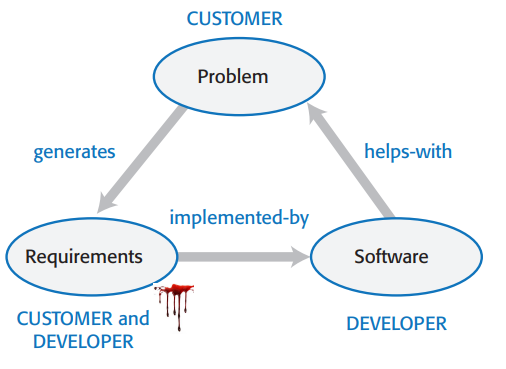
\includegraphics[width=0.65\textwidth]{image01}
	\caption{The 23 Design Patterns of the Gang of Four; Erich Gamma, Richard Helm, Ralph Johnson and John Vlissides, Design Patterns: Elements of Reusable Object-Oriented Software (1995).}
	\label{image01}
\end{figure}
The starting point for the software development is a set of \textit{‘software
	requirements’} that are owned by an external client and which set out what they want a software system to do to support their business processes.
The software is developed by a software company (the contractor) who design and implement a system that delivers functionality to meet the requirements. The customer may change the requirements at any time in response to business changes (they usually do). The contractor must change the software to reflect these requirements changes. Custom software usually has a long-lifetime (10 years or more) and it must be supported over that lifetime.
Another paradigms is represented by \textbf{product-based Software Engineering} as pictured in \ref{image02}

\begin{figure}[h]
	\centering
	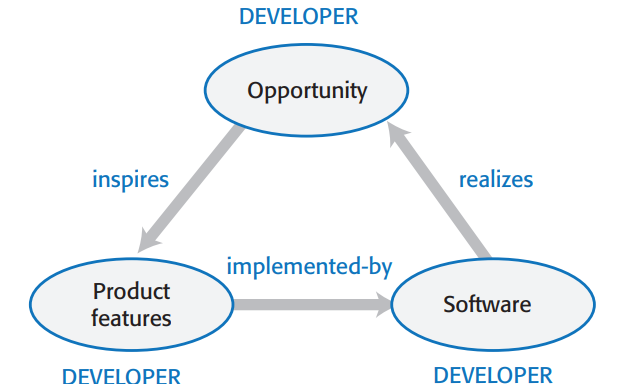
\includegraphics[width=0.65\textwidth]{image02}
	\caption{Here developer decides product features and following evolutions}
	\label{image02}
\end{figure}

The starting point for product development is a business opportunity thatis identified by individuals or a company. They develop a software product to take advantage of this opportunity and sell this to customers. The company who identified the opportunity design and implement a setof software features that realize the opportunity and that will be useful to
customers.The software development company are responsible for deciding on the development timescale, what features to include and when the product should change. Rapid delivery of software products is essential to capture the market for that type of product.

This two type of SE can define also the \textbf{Software Execution models}:
\begin{itemize}
	\item \textit{Stand-alone}: The software executes entirely on the customer’s
	computers.
	\item \textit{Hybrid}: Part of the software’s functionality is implemented on the
	customer’s computer but some features are implemented on the product
	developer’s servers.
	\item \textit{Software service}:All of the product’s features are implemented on the
	developer’s servers and the customer accesses these through a browser
	or a mobile app.
\end{itemize}

\begin{figure}[h]
	\centering
	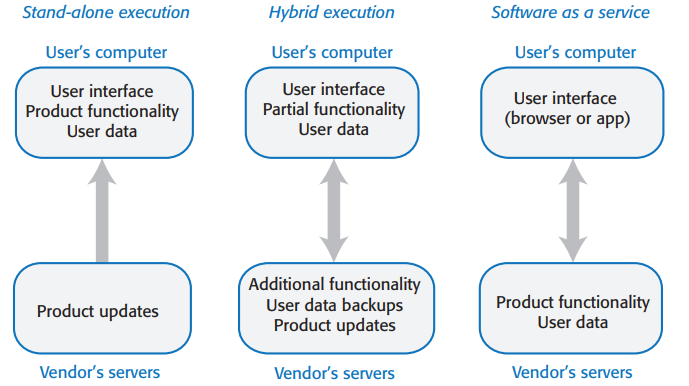
\includegraphics[width=0.65\textwidth]{image03}
	\caption{Here developer decides product features and following evolutions}
	\label{image03}
\end{figure}

\section{Product vision}
The starting point for software product development is a ‘product vision’. Product visions are simple statements that define the essence of the product to be developed.
The product vision should answer three fundamental questions:

\begin{itemize}


\item What is the product to be developed?

\item Who are the target customers and users?

\item Why should customers buy this product?
\end{itemize}
This allow to present a general template, pictured in \ref{image04} and some examples in \ref{image05}. The product vision is determined by:
\begin{itemize}
	\item \textit{Domain experience}: The product developers may work in a particular area (say marketing and sales) and understand the software support that they need. They may be frustrated by the deficiencies
	in the software they use and see opportunities for an improved system
	\item \textit{Product experience}:Users of existing software (such as word processing software) may see simpler and better
	ways of providing comparable functionality and propose a new system that implements this.
	New products can take advantage of recent technological developments such as speech
	interfaces.
	\item \textit{Customer experience}: The software developers may have extensive discussions with prospective customers of
	the product to understand the problems that they face, constraints, such as interoperability,
	that limit their flexibility to buy new software, and the critical attributes of the software that
	they need.
	\item \textit{Prototyping and playing around}:Developers may have an idea for software but need to develop a better understanding of
	that idea and what might be involved in developing it into a product. They may develop a
	prototype system as an experiment and ‘play around’ with ideas and variations using that
	prototype system as a platform.
\end{itemize}


\begin{figure}[h]
	\centering
	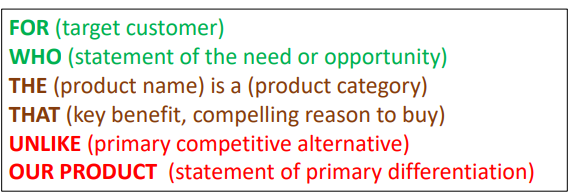
\includegraphics[width=0.7\textwidth]{image04}
	\caption{Here developer decides product features and following evolutions}
	\label{image04}
\end{figure}

\begin{figure}[h]
	\centering
	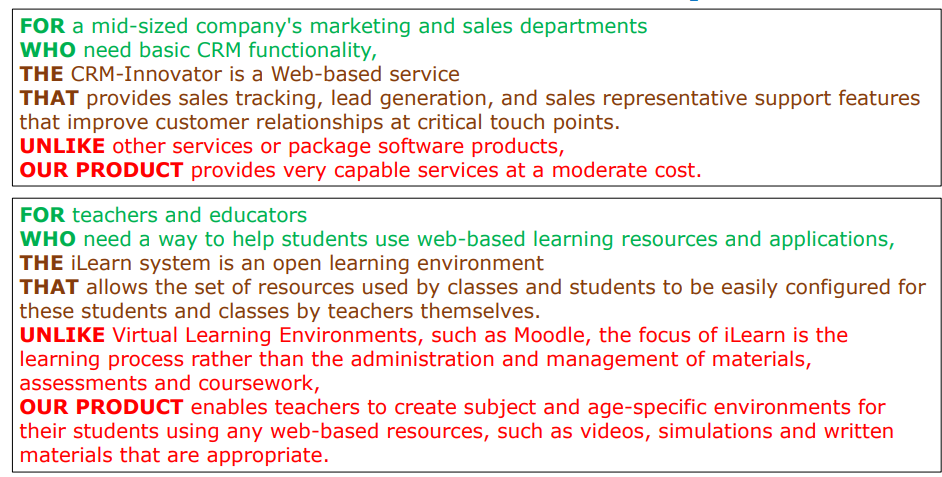
\includegraphics[width=0.7\textwidth]{image05}
	\caption{Here developer decides product features and following evolutions}
	\label{image05}
\end{figure}

\section{Software Product Management}
Software product management is a business activity that focuses on the
software products developed and sold by the business. Product managers (PMs) take overall responsibility for the product and are involved in planning, development and product marketing.
Product managers are the interface between the organization, its customers and the software development team. They are involved at all stages of a product’s lifetime from initial conception through to withdrawal of the product from the market. Product managers must look outward to customers and potential customers rather than focus on the software being developed.
\begin{figure}[h]
	\centering
	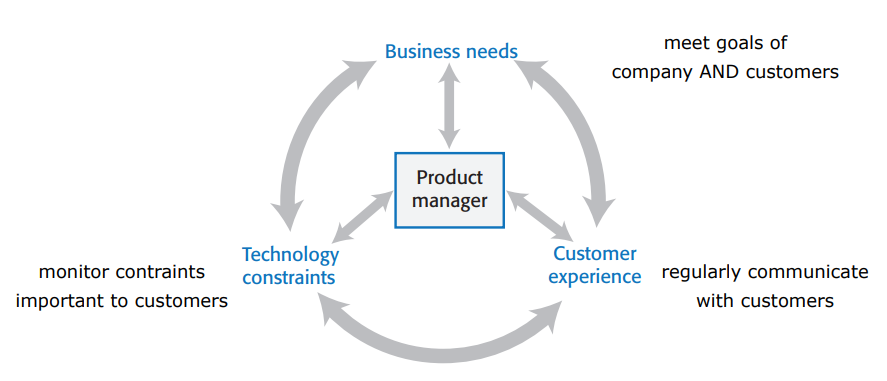
\includegraphics[width=0.7\textwidth]{image06}
	\caption{Here developer decides product features and following evolutions}
	\label{image06}
\end{figure}
Product management concerns
\begin{itemize}
	\item Business needs: PMs have to ensure that the software being developed
	meets the business goals of the software development company.
	\item Technology constraints: PMs must make developers aware of
	technology issues that are important to customers.
	\item Customer experience: PMs should be in regular contact with customers
	and potential customers to understand what they are looking for in a
	product, the types of users and their backgrounds and the ways that the
	product may be used.
	
\end{itemize}

Technical interactions of PMs are:
\begin{itemize}
	\item Product roadmap (set goals, milestones, success criteria)
	\item User story and scenario (to identify product features)
	\item Product backlog (to-do list to complete project development)
	\item Acceptance testing (to verify that release meets set goals)
	\item Customer testing (to get feedback on usability \& fit of features)
	\item UI design (monitor simplicity/naturality)
\end{itemize}

\section{Product prototyping}
Product prototyping is the process of developing an early version of a product
to test your ideas and to convince yourself and company funders that your
product has real market potential.
You may be able to write an inspiring product vision, but your potential users can only
really relate to your product when they see a working version of your software. They can
point out what they like and don’t like about it and make suggestions for new features.

A prototype may be also used to help identify fundamental software components or
services and to test technology. Building a prototype should be the first thing that you do when developing a software product. Your aim should be to have a working version of your
software that can be used to demonstrate its key features. You should always plan to throw-away the prototype after development and to re-implement the software, taking account of issues such as security and reliability.

There are \textbf{two stages} of prototyping, allowing to have a first-reduce prototype in 6 weeks:
\begin{itemize}
	\item \textit{Feasability demonstration}: You create an executable system that
	demonstrates the new ideas in your product. The aims at this stage are
	to see if your ideas actually work and to show funders and/or company
	management the original product features that are better than those in
	competing products.
	
	\item \textit{Customer demonstration}:  You take an existing prototype created to
	demonstrate feasibility and extend this with your ideas for specific
	customer features and how these can be realized. Before you develop
	this type of prototype, you need to do some user studies and have a
	clearer idea of your potential users and scenarios of use.
\end{itemize} 

\chapter{Agile Software Engineering}
Software products must be brought to market quickly so rapid software development and delivery is essential. Virtually all software products are now developed using an agile approach.Agile software engineering focuses on delivering functionality quickly, responding to changing product specifications and minimizing
development overheads.
A large number of ‘agile methods’ have been developed: there is no ‘best’ agile method or technique. It depends on who is using the technique, the development team and the type of product being developed.

Plan-driven development evolved to support the engineering of large, long-lifetime systems (such as aircraft control systems) where teams may be geographically dispersed and work on the software for several years.
This approach is based on controlled and rigorous software development processes that include detailed project planning, requirements specification and analysis and system modelling.
However, plan-driven development involves significant overheads anddocumentation and it does not support the rapid development and delivery of software.
Agile methods were developed in the 1990s to address this problem: these methods focus on the software rather than its documentation, develop software in a series of increments and aim to reduce process bureaucracy as much as possible.
The \textbf{Agile manifesto} state that: 
\textquote{We are uncovering better ways of developing software by doing it and
	helping others to do it. Through this work, we have come to value:
	\begin{itemize}
		

	\item individuals and interactions over processes and tools;
	\item working software over comprehensive documentation;
	\item customer collaboration over contract negotiation;
	\item responding to change over following a plan.
		\end{itemize}
	While there is value on the items on the right, we value the items on
	the left more.}

All agile methods are based around incremental development and delivery. Product development focuses on the software featues, when a featue does something for the software user. With incremental development, you start by prioritizing the features so that the most important features are implemented first:
you only define the details of the feature being implemented in an increment. That feature is then implemented and delivered.
Users or surrogate users can try it out and provide feedback to the development team. You then go on to define and implement the next feature of the system as pictured in \ref{image07}-
\begin{figure}[h]
	\centering
	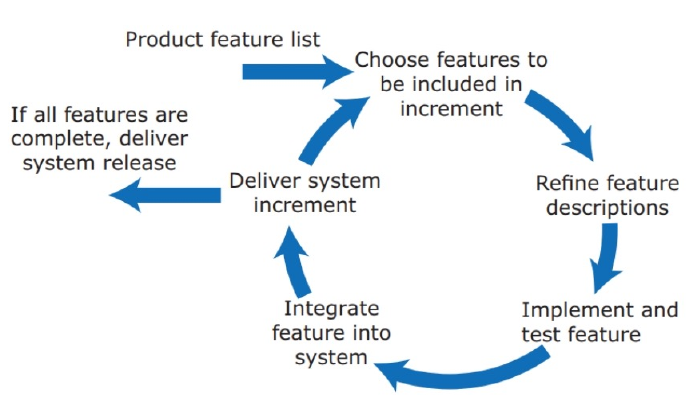
\includegraphics[width=0.7\textwidth]{image07}
	\caption{Here developer decides product features and following evolutions}
	\label{image07}
\end{figure}
That process can be syntethized by following these twelve principles:

\begin{enumerate}
\item Our highest priority is to satisfy the customer through early and continuous delivery of
valuable software.
\item  Welcome changing requirements, even late in development. Agile processes harness change
for the customer's competitive advantage.
\item  Deliver working software frequently, from a couple of weeks to a couple of months, with
a preference to the shorter timescale.
\item  Business people and developers must work together daily throughout the project.
\item  Build projects around motivated individuals. Give them the environment and support they
need, and trust them to get the job done.
\item  The most efficient and effective method of conveying information to and within a
development team is face-to-face conversation.
\item  Working software is the primary measure of progress.
\item  Agile processes promote sustainable development. The sponsors, developers, and users should
be able to maintain a constant pace indefinitely.
\item  Continuous attention to technical excellence and good design enhances agility.
\item  Simplicity--the art of maximizing the amount of work not done--is essential.
\item  The best architectures, requirements, and designs emerge from self-organizing teams.
\item  At regular intervals, the team reflects on how to become more effective, then tunes and
adjusts its behavior accordingly.
\end{enumerate}

\section{Extreme programming}
The most influential work that has changed software development culture
was the development of Extreme Programming (XP). The name was coined by Kent Beck in 1998 because the approach was developed by pushing recognized good practice, such as iterative
development, to ‘extreme’ levels.
Extreme programming focused on 12 new development techniques, pictured in \ref{image08}, that were geared to rapid, incremental software development, change and delivery. Some of these techniques are now widely used; others have been less popular.

\begin{figure}[h]
	\centering
	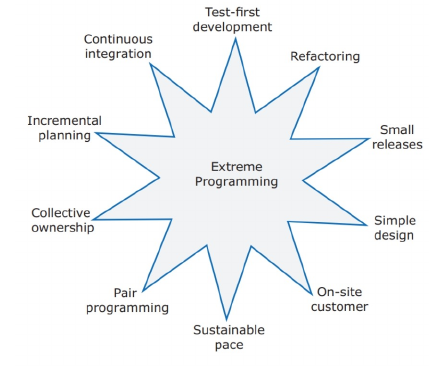
\includegraphics[width=0.7\textwidth]{image08}
	\caption{Here developer decides product features and following evolutions}
	\label{image08}
\end{figure}
\begin{itemize}
	\item Incremental planning/user stories: There is no ‘grand plan’ for the system. Instead, what needs to be implemented (the requirements) in each increment are established in
	discussions with a customer representative. The requirements are written
	as user stories. The stories to be included in a release are determined by
	the time available and their relative priority.
	\item Small releases: The minimal useful set of functionality that provides business value is
	developed first. Releases of the system are frequent and incrementally
	add functionality to the previous release.
	\item Test-driven development: Instead of writing code then tests for that code, developers write the
	tests first. This helps clarify what the code should actually do and that
	there is always a ‘tested’ version of the code available. An automated unit
	test framework is used to run the tests after every change. New code
	should not ‘break’ code that has already been implemented.
	\item Continuous integration: As soon as the work on a task is complete, it is integrated into the
	whole system and a new version of the system is created. All unit
	tests from all developers are run automatically and must be
	successful before the new version of the system is accepted.
	\item Refactoring: Refactoring means improving the structure, readability, efficiency and
	security of a program. All developers are expected to refactor the
	code as soon as potential code improvements are found. This keeps
	the code simple and maintainable.
\end{itemize}



\section{Scrum}
Software company managers need information that will help them understand how much it costs to develop a software product, how long it will take and when the product can be brought to market.
Plan-driven development provides this information through long-term development plans that identify deliverables - items the team will deliver and when these will be delivered.Plans always change so anything apart from short-term plans
are unreliable.


Scrum is a lightweight framework that helps people, teams and organizations generate value through adaptive solutions for
complex problems.
The Scrum Framework contains a set of principles and rules to following order to achieve a common goal.


Scrum is founded on \textbf{empiricism}, it asserts that knowledge comes from experience
and making decisions based on what is observed
and \textbf{lean thinking}: it reduces waste and focuses on the essentials.
Scrum employs an iterative, incremental approach to optimize predictability and to control risk.

The Scrum theory \textbf{pillars} are:
\begin{itemize}
	\item Transparency: The emergent process and work must be visible to those performing
	the work as well as those receiving the work.
	
	\item Inspection: Scrum artifacts and the progress toward agreed goals must be
	inspected frequently and diligently to detect potentially undesirable
	variances or problems.
	
	\item Adaptation:If any aspects of a process deviate outside acceptable limits or if the
	resulting product is unacceptable, the process being applied or the
	materials being produced must be adjusted. The adjustment must be
	made as soon as possible to minimize further deviation.
	
	\item 
\end{itemize}

Successful use of Scrum depends on people becoming
more proficient in living five values: \textit{Commitment, Focus, Openness, Respect, Courage}.

\section{Scrum in practice}
The scrum's main actors are:
\begin{itemize}
	\item Scrum team: composed by Product owner, Scrum Master, Developers
	
	\item Artifacts: composed by Product backlog, Sprint backlog
	
	\item Scrum events: Sprint planning, execution and review
\end{itemize}

There are two main key roles in Scrum. The firstone is the \textbf{Product owner} that is responsible for ensuring that the development
team are always focused on the product they are building rather than diverted into technically interesting but less relevant work. In product development, the product manager should normally take on the Product Owner role.
The second one is the \textbf{Scrum master} that is a Scrum expert whose job is to guide the team in the effective use of the Scrum method. The developers of Scrum emphasize that the ScrumMaster is not a conventional project manager
but is a coach for the team. They have authority within the team on how Scrum is used.
In many companies that use Scrum, the ScrumMaster also has some project management responsibilities.

\subsection{Scrum in Sprints}
In Scrum, software is developed in sprints, which are fixed-length periods (2 - 4 weeks) in which software features are developed and
delivered. During a sprint, the team has daily meetings (Scrums) to review progress
and to update the list of work items that are incomplete. Sprints should produce a ‘shippable product increment’. This means that the developed software should be complete and ready to deploy.

\begin{figure}[h]
	\centering
	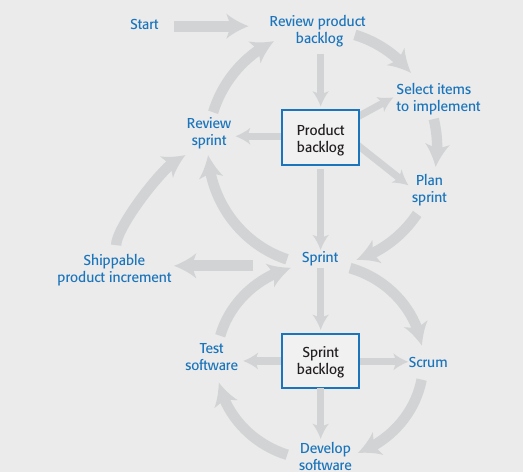
\includegraphics[width=0.7\textwidth]{image09}
	\caption{Scrum cycles}
	\label{image09}
\end{figure}

The \textbf{Product backlog} is a to-do list of items to be implemented that is reviewed and
updated before each sprint. The \textbf{sprints are timeboxed} in a fixed-time (2-4 week) periods in which items from the product backlog are implemented. Also teams are \textbf{self-organized}, making their own decisions and work by discussing issues and making decisions by consensus.

The \textbf{product backlog} is a list of what needs to be done to complete the
development of the product. The items on this list are called product backlog items (PBIs).
The product backlog may include a variety of different items such as product features to be implemented, user requests, essential development activities and desirable engineering improvements.
The product backlog should always be prioritized so that the items that be implemented first are at the top of the list. This is an example of \textbf{product backlog items}:
\begin{enumerate}
	
	\item As a teacher, I want to be able to configure the group of tools that
	are available to individual classes. (feature)
	
	\item As a parent, I want to be able to view my childrens’ work and the
	assessments made by their teachers. (feature)
	
	\item As a teacher of young children, I want a pictorial interface for
	children with limited reading ability. (user request)
	
	\item  Establish criteria for the assessment of open source software that
	might be used as a basis for parts of this system. (development activity)
	
	\item  Refactor user interface code to improve understandability and
	performance. (engineering improvement)
	
	\item  Implement encryption for all personal user data. (engineering
	improvement)
\end{enumerate}

The product backlog item states:
\begin{itemize}
	\item Ready for consideration: these are high-level ideas and feature descriptions that will be
	considered for inclusion in the product. They are tentative so may
	radically change or may not be included in the final product.
	
	\item Ready for refinement: the team has agreed that this is an important item that should be
	implemented as part of the current development. There is a
	reasonably clear definition of what is required. However, work is
	needed to understand and refine the item.
	
	\item Ready for implementation: the PBI has enough detail for the team to estimate the effort involved
	and to implement the item. Dependencies on other items have been
	identified.
\end{itemize}


\begin{figure}[h]
	\centering
	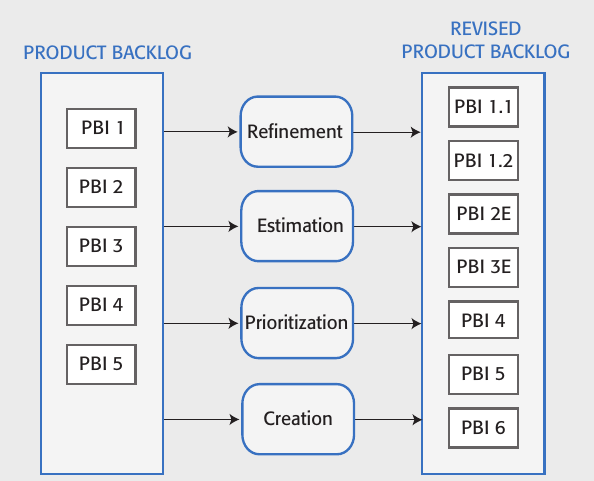
\includegraphics[width=0.7\textwidth]{image10}
	\caption{Scrum cycles}
	\label{image10}
\end{figure}
 
The main \textbf{product backlog activities} are concentrated on:
\begin{itemize}
	\item Refinement: Existing PBIs are analysed and refined to create more detailed PBIs. This may
	lead to the creation of new product backlog items.
	\item Estimation: The team estimate the amount of work required to implement a PBI and add this
	assessment to each analysed PBI.
	\item Creation: New items are added to the backlog. These may be new features suggested by
	the product manager, required feature changes, engineering improvements, or process activities such as the assessment of development tools that might be used.
	\item Priorization: The product backlog items are reordered to take new information and changed
	circumstances into account.
\end{itemize} 
 
\subsection{PBI estimation metrics}
The two main metrics are:
\begin{itemize}
	\item \textbf{Effort required}:This may be expressed in person-hours or person-days i.e. the number of hours or days it would take one person to implement that PBI. This is not the same as
	calendar time. Several people may work on an item, which may shorten the
	calendar time required.
	
	\item \textbf{Story points}: Story points are an arbitrary estimate of the effort involved in implementing a PBI, taking into account the size of the task, its complexity, the technology that
	may be required and the ‘unknown’ characteristics of the work.
	They were derived originally by comparing user stories, but they can be used for
	estimating any kind of PBI. Story points are estimated relatively. The team agree on the story points for a baseline task and other tasks are estimated by comparison with this e.g. more/less complex, larger/smaller etc.
\end{itemize}

\section{Sprint activities and planning}
 Products are developed in a series of sprints, each of which delivers an increment of the product or supporting software.Sprints are short duration activities (2-4 weeks) and take place between
a defined start and end date. Sprints are timeboxed, which means that development stops at the end of a sprint whether or not the work has been completed. During a sprint, the team work on the items from the product backlog.

We can distinguish three main activities (in picture \ref{image11}):
\begin{itemize}
	\item Sprint planning: Work items to be completed in that sprint are selected and, if necessary,
	refined to create a sprint backlog. This should not last more than a day at
	the beginning of the sprint.
	\item Sprint execution:	The team work to implement the sprint backlog items that have been
	chosen for that sprint. If it is impossible to complete all of the sprint
	backlog items, the sprint is not extended. The unfinished items are
	returned to the product backlog and queued for a future sprint.
	\item Sprint reviewing: The work done in the sprint is reviewed by the team and (possibly)
	external stakeholders. The team reflect on what went well and what went
	wrong during the sprint with a view to improving their work process.
\end{itemize}
\begin{figure}[h]
	\centering
	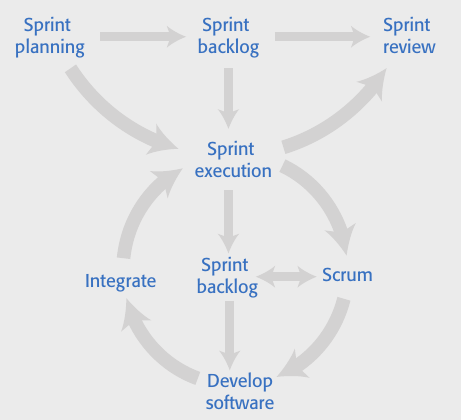
\includegraphics[width=0.7\textwidth]{image11}
	\caption{Scrum cycles}
	\label{image11}
\end{figure}

\subsection{Sprint planning}
Allows to establish an agreed sprint goal: Sprint goals may be focused on software functionality, support or performance and reliability. Decide on the list of items from the product backlog that should be
implemented, then create a sprint backlog: this is a more detailed version of the product backlog that records the work to be done during the sprint.
\begin{figure}[h]
	\centering
	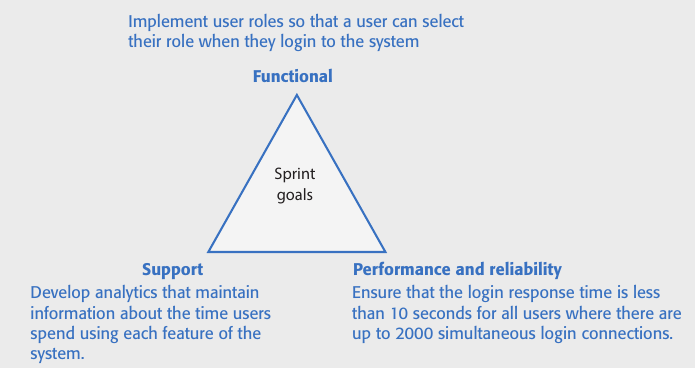
\includegraphics[width=0.7\textwidth]{image12}
	\caption{Scrum cycles}
	\label{image12}
\end{figure}

In a sprint plan, the team decides which items in the product backlogshould be implemented during that sprint. Key inputs are the effort estimates associated with PBIs and the team’s velocity.
The output of the sprint planning process is a sprint backlog.: is a breakdown of PBIs to show the what is involved in implementing the PBIs chosen for that sprint. During a sprint, the team have daily meetings (scrums) to coordinate their work.

A scrum is a short, daily meeting that is usually held at the beginning of the day. During a scrum, all team members share information, describe their progress since the previous day’s scrum, problems that have arisen
and plans for the coming day. This means that everyone on the team knows what is going on and, if problems arise, can re-plan short-term work to cope with them.

Scrum meetings should be short and focused. To dissuade team members from getting involved in long discussions, they are sometimes organized as ‘stand-up’ meetings where there are no chairs in the
meeting room.


During a scrum, the sprint backlog is reviewed. Completed items are removed from it. New items may be added to the backlog as new information emerges. The team then decide who should work on sprint backlog items that day.

Scrum does not suggest the technical agile activities that should be used. However, there are two practices that are strongly suggested by agile software engineers to be used in a sprint:
\begin{itemize}
	\item Test automation: As far as possible, product testing should be automated. You should develop a suite of executable tests that can be run at any time.
	
	\item Continous integration: Whenever anyone makes changes to the software components they are developing, these components should be immediately integrated with other components to create a system. This system should then be tested to check for unanticipated component interaction problems.
\end{itemize}

At the end of each sprint, there is a review meeting, which involves the
whole team. This meeting allows to reviews whether or not the sprint has met its goal,sets out any new problems and issues that have emerged during the sprint. This is a way for a team to reflect on how they can improve the way they work.
The product owner has the ultimate authority to decide whether or not the goal of the print has been achieved. They should confirm that the implementation of the selected product backlog items is complete.

The sprint review should include a process review, in which the team reflects on its own way of working and how Scrum has been used. The aim is to identify ways to improve and to discuss how to use Scrum more productively, following the self-organizing team philosphy \ref{image13}.
\begin{figure}[h]
	\centering
	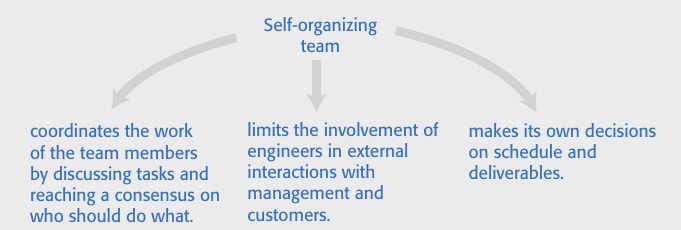
\includegraphics[width=0.7\textwidth]{image13}
	\caption{Scrum cycles}
	\label{image13}
\end{figure}

\subsection{Team composition and coordination}
The ideal Scrum team size is between 5 and 8 people: teams have to tackle diverse tasks and so usually require people with different skills, such as networking, user experience, database design and so on.

They usually involve people with different levels of experience.A team of 5-8 people is large enough to be diverse yet small enough to communicate informally and effectively and to agree on the priorities of the
team.
The advantage of a self-organizing team is that it can be a cohesive team that can adapt to change.
Because the team rather than individuals take responsibility for the work, they can cope with people leaving and joining the team. Good team communication means that team members inevitably learn something about each other’s areas.

The developers of Scrum assumed that teams would be co-located. They would work in the same room and could communicate informally. Daily scrums mean that the team members know what’s been done and what
others are doing.
 However, the use of daily scrums as a coordination mechanism is based on two assumptions that are not always correct:
 \begin{itemize}
 	\item Scrum assumes that the team will be made up of full-time workers who share a
 	workspace. In reality, team members may be part-time and may work in
 	different places. For a student project team, the team members may take
 	different classes at different times.
 	
 	\item Scrum assumes that all team members can attend a morning meeting to
 	coordinate the work for the day. However, some team members may work
 	flexible hours (e.g. because of childcare responsibilities) or may work on several
 	projects at the same time.
 \end{itemize}
The \textbf{External interactions} are interactions that team members have with people outside of the team.
In Scrum, the idea is that developers should focus on development and only the ScrumMaster and Product Owner should be involved in external interactions. The intention is that the team should be able to work on software development without external interference or distractions.
\begin{figure}[h]
	\centering
	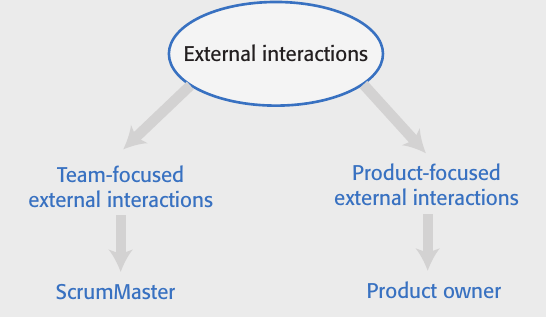
\includegraphics[width=0.7\textwidth]{image14}
	\caption{Scrum cycles}
	\label{image14}
\end{figure}

\section{Project management}
In all but the smallest product development companies, there is a need for development teams to report on progress to company management.
A self-organizing team has to appoint someone to take on these responsibilities: because of the need to maintain continuity of communication with people outside of the group, rotating these activities around team members is not aviable approach.
The developers of Scrum did not envisage that the ScrumMaster should also have project management responsibilities: in many companies, however, the ScrumMaster has to take on project
management responsibilities.They know the work going on and are in the best position to provide accurate
information and project plans and progress.
\begin{figure}[h]
	\centering
	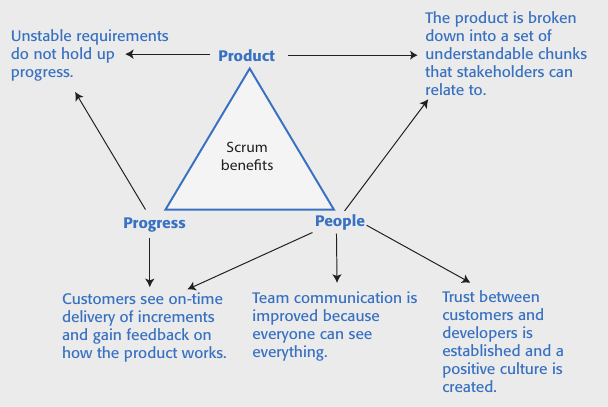
\includegraphics[width=0.7\textwidth]{image15}
	\caption{Scrum cycles}
	\label{image15}
\end{figure}

\chapter{Scenarios, personas \& stories}
The factors driving the design of software products are \textit{inspiration, business/consumer needs to met by existing products, dissatisfaction with existing products and technical changes making new product types possible.}

Product-based software engineering needs less requirements documentation that project-based software engineering because requirements not set by customers
and requirements can change.

Identify product features (= fragments of functionality) instead need to understand potential users by interviews/surveys, informal user analysis/consultations. Remember that business managers buy product, employee (may not
want to) use it. 

User representations (\textbf{personas}) and natural language descriptions (\textbf{scenarios and stories}) help identifying product \textbf{features.}
\begin{figure}[h]
	\centering
	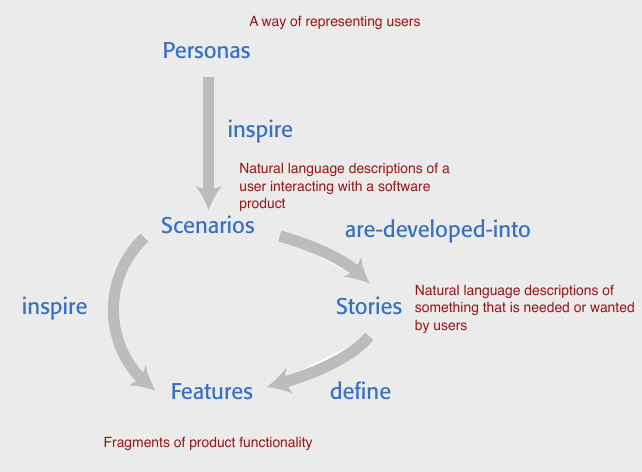
\includegraphics[width=0.7\textwidth]{image16}
	\caption{Scrum cycles}
	\label{image16}
\end{figure}

\section{Personas}
\textit{Who are the target users for our product?}
Need to understand potential users to design features useful for them by identifying the background, skills and experience of potential users.
Personas are (imagined) types of product users: for a dentist agenda: dentist, receptionist, patient.
Generally we need a few (1-2, max 5) personas to identify key product features.


\begin{itemize}
	\item Personalization: You should give them a name and say something about their personal
	circumstances. This is important because you shouldn’t think of a persona as a
	role but as an individual. It is sometimes helpful to use an appropriate stock
	photograph to represent the person in the persona. Some studies suggest that this
	helps project teams use personas more effectively.
	\item Job-related: If your product is targeted at business, you should say something about their job
	and (if necessary) what that job involves. For some jobs, such as a teacher where
	readers are likely to be familiar with the job, this may not be necessary.
	\item Education: You should describe their educational background and their level of technical skills
	and experience. This is important, especially for interface design.
	\item Relevance: If you can, you should say why they might be interested in using the product and
	what they might want to do with it.
\end{itemize}
\begin{figure}[h]
	\centering
	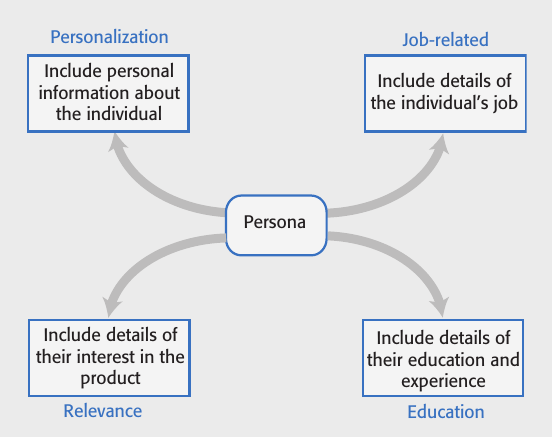
\includegraphics[width=0.7\textwidth]{image17}
	\caption{Scrum cycles}
	\label{image17}
\end{figure}
It is sometimes helpful to use an appropriate \textbf{stock photograph} to represent the person in the persona. Some studies suggest
that this helps project teams use personas moreeffectively.
Using photos is misleading:ersonas shouldn’t be about how people look, but what they do. (Steve Cable)
Detailed personas encouraged the team to assume that demographic information drove motivations. (Sara Wachter-Boettcher).
Persona profiles with a smiling photo result in an increase in willingness to use the personas. (Joni Salminen et al.). Gender has a mediating influence on perceived attributes of males and females. (Francine M. Deutsch)

An example of persona that doesn't have a technical background and wants only a product that support administration is in \ref{image18}.

\begin{figure}[h]
	\centering
	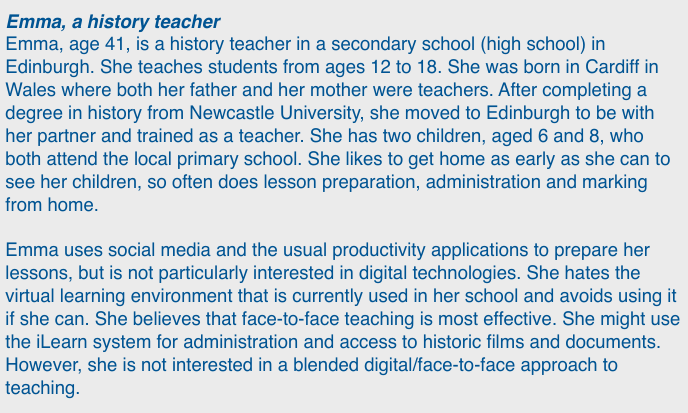
\includegraphics[width=0.7\textwidth]{image18}
	\caption{Scrum cycles}
	\label{image18}
\end{figure}

Personas allow developers to “step into the users’shoes”: when studying the users is not possible (e.g. for some new products) we can develop \textbf{proto-personas}.

\section{Scenarios}
A scenario allow to discover product features, we can define scenarios of user interactions with the product
Scenario = narrative describing a situation in which a user is using our product’s features to do something she wants to do. 
In figure \ref{image19} an example. 
\begin{figure}[h]
	\centering
	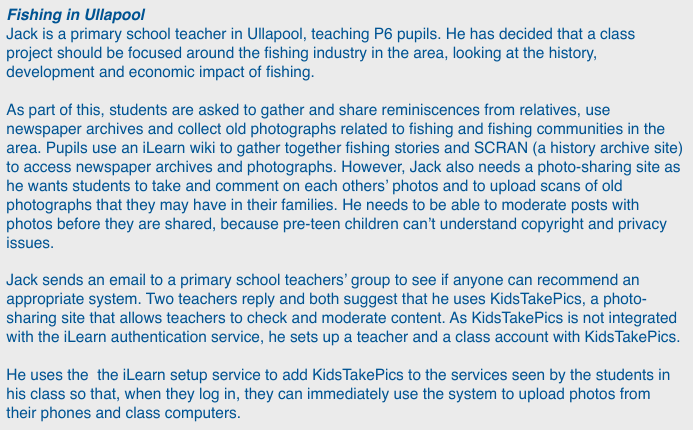
\includegraphics[width=0.7\textwidth]{image19}
	\caption{Scrum cycles}
	\label{image19}
\end{figure}
 So, a \textbf{scenario} is a narrative, high-level scenarios facilitate communication and
 stimulate design creativity. Scenarios are not specifications, though (they lack detail and  may be incomplete). Generally 3-4 scenarios for each persona are suggested, allow to cover main responsabilities of persona. They're written from user's perspective: each team member should individyally create some scenarios, and then discuss them with rest of team and with user (if possible). 
 
 \section{User stories}
 Differently from scenarios, an \textbf{user stories} are finer-grain narratives that set out in a more detailed and structured way a single thing that a user wants from a software system, as stated in \ref{image20}.
 User stories should focus on a clearly defined system feature or aspect of a feature that can be implemented within a single sprint: if the story is about a more complex feature that might take several sprints to implement, then it is called an \textbf{epic}.
 
 \textit{"As a system manager, I need a way to backup the system and restore either individual applications, files, directories or the whole system"}: there is a lot of functionality associated with this user story. For implementation, it should be broken down into simpler stories with each story focusing on a single aspect of the backup system.
 
 You can develop user stories by refining scenarios: three user stories can be identified from the following fragment of Emma’s scenario, as pictured in \ref{image20}.
 
 \textit{"
 From home, she logs onto the iLearn system using her Google account
 credentials. Emma has two iLearn accounts – her teacher account and a parent
 account associated with the local primary school. The system recognises that
 she is a multiple account owner and asks her to select the account to be used.
 She chooses the teacher account and the system generates her personal
 welcome screen. As well as her selected applications, this also shows
 management apps that help teachers create and manage student groups."}
\begin{figure}[h]
	\centering
	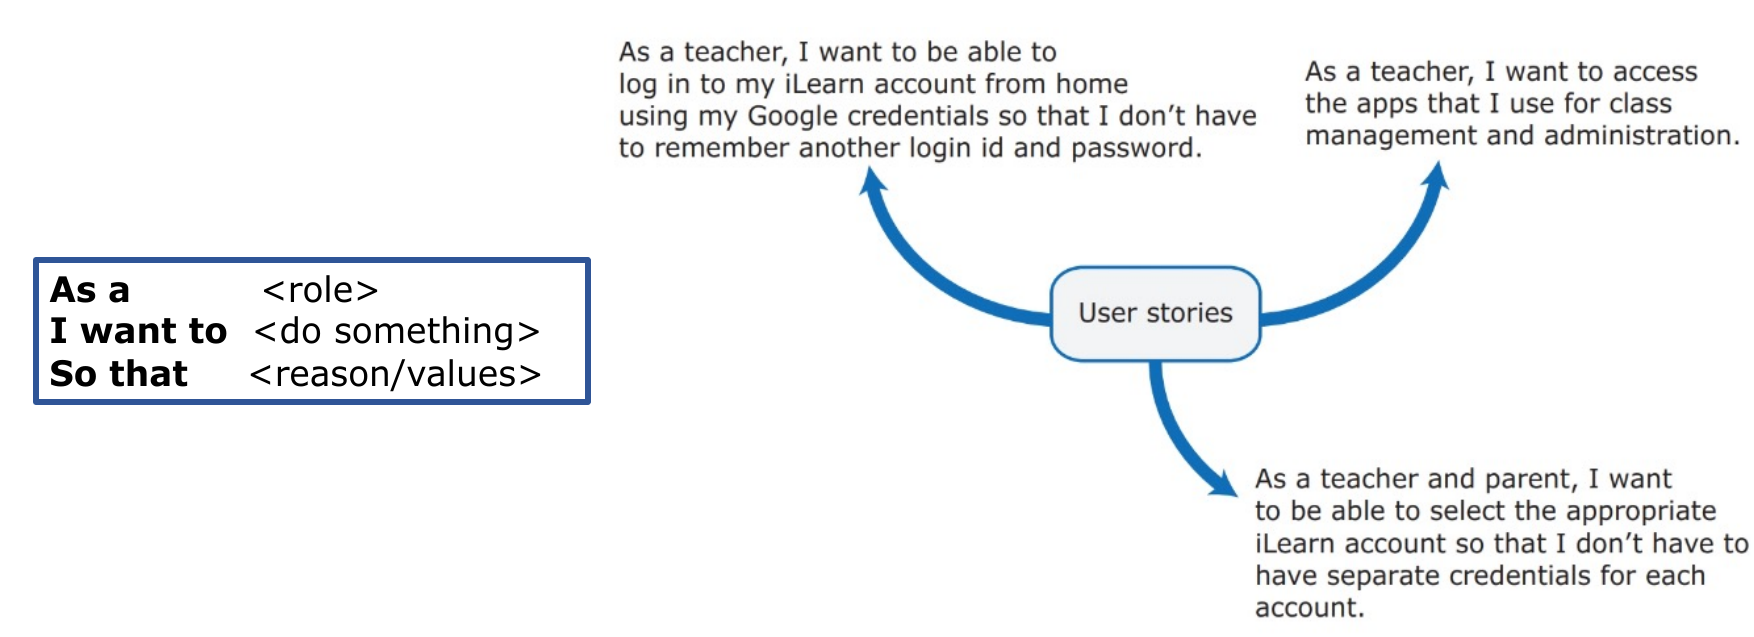
\includegraphics[width=0.7\textwidth]{image20}
	\caption{Scrum cycles}
	\label{image20}
\end{figure}


Stories are associated with priorities (and possibly
also with an estimate of effort needed to implement
the story) and sorted according to priority
(\textbf{requirements triage}).

It is possible to express all the functionalities described in a scenario as user stories but scenarios can be read more naturally, make it easir to understand stories and provide more context.

\subsection{Feature identification}
Your aim in the initial stage of product design should be to create a list of
features that define your product.
A feature is a way of allowing users to access and use your product’s functionality so the feature list defines the overall functionality of the system.
Features should be:
\begin{itemize}
	\item Independence: features should not depend on how other system features are implemented and
	should not be affected by the order of activation of other features.
	
	\item Coherence: features should be linked to a single item of functionality. They should not do more
	than one thing and they should never have side-effects.
	
	\item Relevance: features should reflect the way that users normally carry out some task. They
	should not provide obscure functionality that is hardly ever required.
\end{itemize}

The \textbf{knowledge sources for features design} are multiple like:
\begin{itemize}
	
	\item User knowledge: You can use user scenarios and user stories to inform the team of what users
	want and how they might use it the software features.
	\item Product knowledge: You may have experience of existing products or decide to research what these products do as part of your development process. Sometimes, your features have
	to replicate existing features in these products because they provide fundamental
	functionality that is always required.
	\item Domain knowledge: this is knowledge of the domain or work area(e.g. finance, event booking) that your product aims to support. By understanding the domain, you can think of new
	innovative ways of helping users do what they want to do.
	\item Technology knowledge: new products often emerge to take advantage of technological developments since their competitors were launched. If you understand the latest technology,
	you can design features to make use of it.
\end{itemize}
At the same time, the \textbf{factors} in feature set design are undirectly proportional each other as in \ref{image21}. 
\begin{figure}[h]
	\centering
	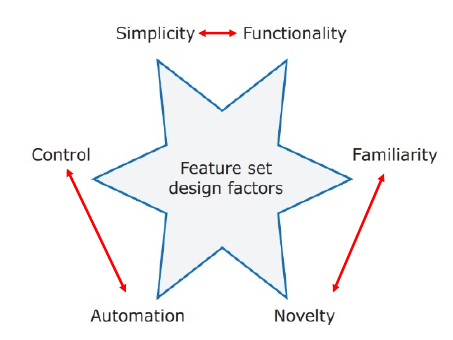
\includegraphics[width=0.7\textwidth]{image21}
	\caption{Scrum cycles}
	\label{image21}
\end{figure}

\subsection{Feature creep}
\textbf{Feature creep} occurs when new features are added in response to user requests without considering whether or not these features are generally
useful or whether they can be implemented in some other way.
 Too many features make products hard to use and understand and there are three reasons why feature creep occurs:
\begin{enumerate}
	\item Product managers are reluctant to say ‘no’ when users ask for specific features.
	\item Developers try to match features in competing products.
	\item The product includes features to support both inexperienced and experienced users.
\end{enumerate}

To avoid feature creep we need to answer the questions pictured in \ref{image22}.
\begin{figure}[h]
	\centering
	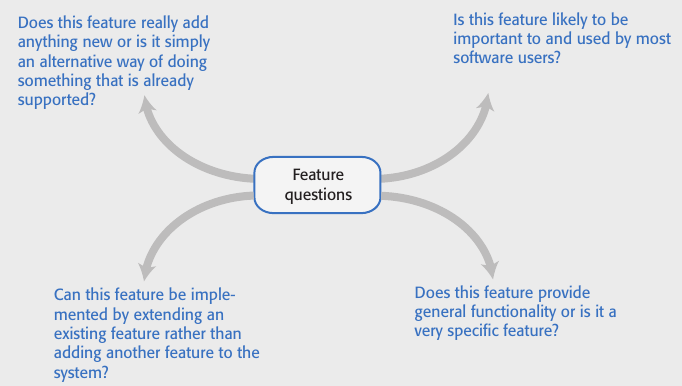
\includegraphics[width=0.7\textwidth]{image22}
	\caption{Scrum cycles}
	\label{image22}
\end{figure}

Features can be identified directly from the product vision or from
scenarios. You can highlight phrases in narrative description to identify features to be included in the software.

\chapter{Software Architecture}
To create a reliable, secure and efficient product, you need to pay attention to architectural design which includes:
\begin{itemize}
	\item its overall organization,
	\item how the software is decomposed into components,
	\item the server organization
	\item the technologies that you use to build the software.The architecture of a software
	product affects its performance, usability, security, reliability and maintainability.
	\end{itemize}
There are many different interpretations of the term ‘software architecture’. We present the \textbf{IEEE definition of software architecture}: \textit{"Architecture is the fundamental organization of a software system embodied in its components, their relationships to each other and to the environment, and the principles guiding its design and evolution."}

\subsection{Components}
A component is an element that implements a coherent set of functionality or features.
Software component can be considered as a collection of one or more services that may be used by other components: when designing software architecture, you don’t have to decide how anarchitectural element or component is to be implemented.Rather, you design the component interface and leave theimplementation of that interface to a later stage of the development. An abstraction in \ref{image23}.

\begin{figure}[h]
	\centering
	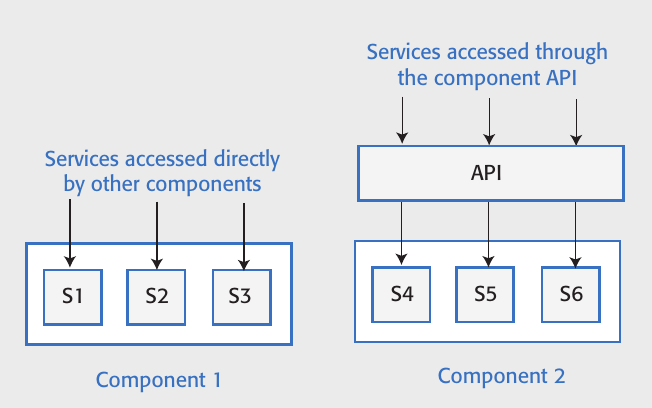
\includegraphics[width=0.7\textwidth]{image23}
	\caption{Scrum cycles}
	\label{image23}
\end{figure}
 There are plenty of issues that influence the architectural decisions, pictured in \ref{image24}:
 \begin{itemize}
 	\item \textbf{Nonfunctional product characteristics}: Nonfunctional product characteristics such as security and performance affect all users. If you get these wrong, your product will is unlikely to be a commercial success. Unfortunately, some characteristics are opposing, so you can only optimize the most
 	important.
 	\item \textbf{Product lifetime}:If you anticipate a long product lifetime, you will need to create regular product revisions.You therefore need an architecture that is evolvable, so that it can be adapted to accommodate new features and technology.
 	\item \textbf{Software reuse}:	You can save a lot of time and effort, if you can reuse large components from other products or open-source software. However, this constrains your architectural choices
 	because you must fit your design around the software that is being reused.
 	\item \textbf{Number of users}:	If you are developing consumer software delivered over the Internet, the number of users	can change very quickly. This can lead to serious performance degradation unless you
 	design your architecture so that your system can be quickly scaled up and down.
 	\item \textbf{Software compatibility}:For some products, it is important to maintain compatibility with other software so that users can adopt your product and use data prepared using a different system. This may limit architectural choices, such as the database software that you can use.
 	
 \end{itemize}
 \begin{figure}[h]
 	\centering
 	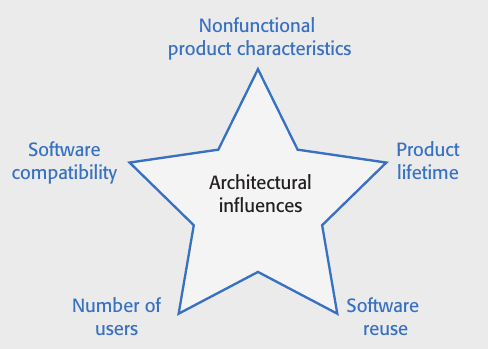
\includegraphics[width=0.7\textwidth]{image24}
 	\caption{Scrum cycles}
 	\label{image24}
 \end{figure}

The main \textbf{non-functional quality attributes} needs to follow these questions to be effective:
\begin{enumerate}
	\item Responsiveness: Does the system return results to users in a reasonable time?
	\item Reliability: Do the system features behave as expected by both developers and users?
	\item Availability:	Can the system deliver its services when requested by users?
	\item Security: Does the system protect itself and users’ data from unauthorized attacks and
	intrusions?
	\item Usability: Can system users access the features that they need and use them quickly and
	without errors?
	\item Maintainability: Can the system be readily updated and new features added without undue costs?
	\item Resilience: Can the system continue to deliver user services in the event of partial failure or
	external attack?
\end{enumerate}
Overall, it's noticeavle to remember that optimizing one non-functional attribute affects others (\textit{like security vs performance usability or availability vs time-to-market semplicity}).
 \begin{figure}[h]
	\centering
	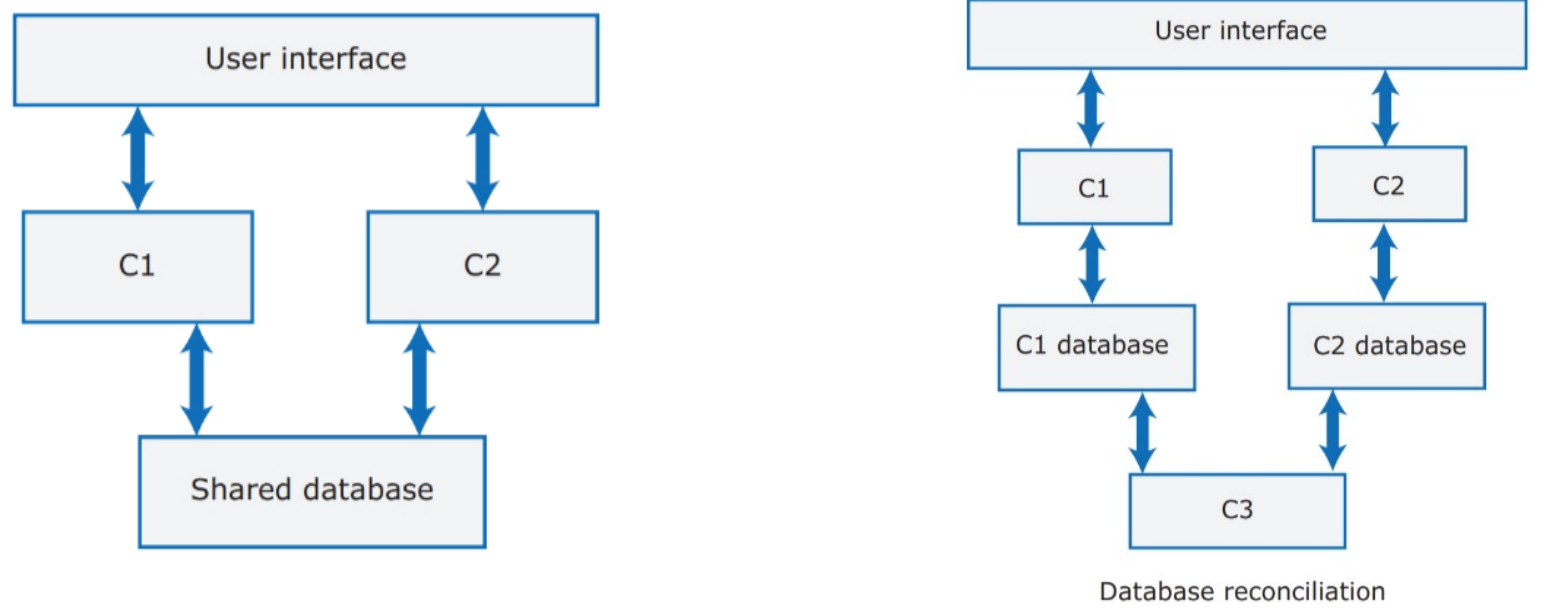
\includegraphics[width=0.7\textwidth]{image25}
	\caption{Scrum cycles}
	\label{image25}
\end{figure}
Let's examine \textbf{mantainability}: it's the difficult/expensiveness to make changes after release. It's a good practice to decompose system into small self-contained parts and avoid shared data structure.
The figure \ref{image25} describe a scenario in which we have initially a \textbf{shared database} but if it fail then the two instances cannot work properly. We can split the database in two (\textit{by some criteria that allows instances to operate almost independently}) and use a thid instance as a reconciliation component. So If one component needs to change the database organization, this does not affect the other component and the system can continue to provide partial service in the event of a database failure, surely at cost of implementing a mechanism for eventual data consistency.

\subsection{System decomposition}
Complexity in a system architecture arises because of the number and the nature of the relationships between components in that system. When decomposing a system into components, you should try to avoid
unnecessary software complexity by \textbf{localize relationships}, if there are relationships between components A and B, these are easier to understand if A and B are defined in the same module and by \textbf{reducing shared dependencies} where components A and B depend on some other component or data,
complexity increases because changes to the shared component mean youhave to understand how these changes affect both A and B.
It is always preferable to use local data wherever possible and to avoid sharing data if you can, as pictured in \ref{image27}. In figure \ref{image26} an example of component relationships.
 \begin{figure}[h]
	\centering
	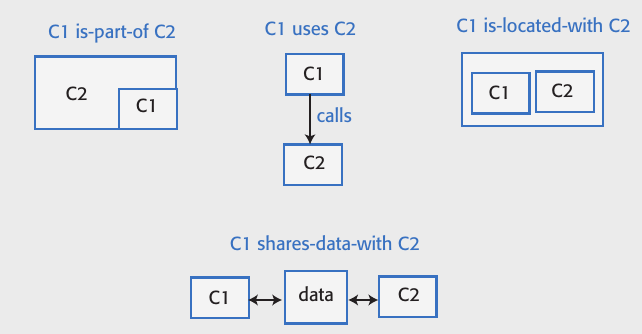
\includegraphics[width=0.7\textwidth]{image26}
	\caption{Scrum cycles}
	\label{image26}
\end{figure}
 \begin{figure}[h]
	\centering
	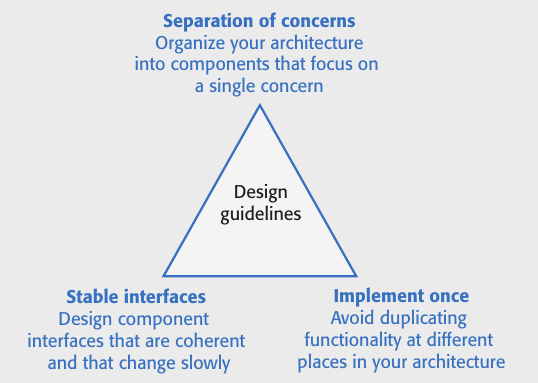
\includegraphics[width=0.7\textwidth]{image27}
	\caption{Scrum cycles}
	\label{image27}
\end{figure}

In a \textbf{layered architecture} each layer is an area of concern and is condiered separately from other layers. Within each layer, the components are independent and do not overlap in functionality. The architectural model is a high-level model that does not include implementation information, as stated in \ref{image28}.
 \begin{figure}[h]
	\centering
	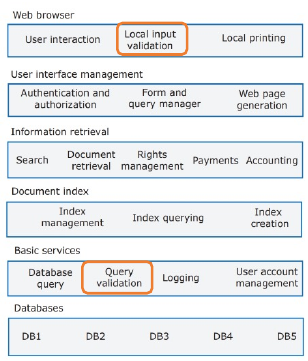
\includegraphics[width=0.7\textwidth]{image28}
	\caption{The orange highlight that concerns may not be always full separated in practice}
	\label{image28}
\end{figure}

\subsubsection{Cross-cutting concerns}
Cross-cutting concerns are concerns that are systemic, that is, they affect
the whole system: in a layered architecture, cross-cutting concerns affect all layers in the system as well as the way in which people use the system.
Cross-cutting concerns are completely different from the functional concerns represented by layers in a software architecture.Every layer has to take them into account and there are inevitably
interactions between the layers because of these concerns.The existence of cross-cutting concerns is the reason why modifying a system after it has been designed to improve its security is often difficult.


In a \textbf{Security architecture} different technologies are used in different layers, such as an SQL database or a Firefox browser. Attackers can try to use of vulnerabilities in these technologies to
gain access. Consequently, you need protection from attacks at each layer as well as protection, at lower layers in the system, from successful attacks that have occurred at higher-level layers.If there is only a single security component in a system, this represents a critical system vulnerability. If all security checking goes through that component and it stops working properly or is compromised in an attack, then you have no reliable security in your system.
By distributing security across the layers, your system is more resilient to attacks and software failure (remember the Rogue One example earlier in the chapter).

In a generic \textbf{web-based application} the layer functionality can be identified into:
\begin{enumerate}
	\item Browser-based or mobile user interface: A web browser system interface in which HTML forms are often used to collect user input. Javascript components for local actions, such as input validation, should also be included at this level. Alternatively, a mobile interface may be implemented as an
	app.
	
	\item Authentication and UI management: A user interface management layer that may include components for user
	authentication and web page generation.
	
	\item Application-specific functionality: An ‘application’ layer that provides functionality of the application. Sometimes, this may be expanded into more than one layer.
	
	\item Basic shared services:A shared services layer, which includes components that provide services used by the application layer components.
	
	\item Database and transaction management: A database layer that provides services such as transaction management and recovery. If your application does not use a database then this may not be required.
\end{enumerate}

Generally speaking, \textit{system decomposition} must be done (partly) in conjunction with
choosing technologies for your system: e.g choice of using relational database affects components at higher layers or choice of supporting interfaces on mobile devices calls for using corresponding UI
development toolkits.

\section{Distribution architecture}
The distribution architecture of a software system defines the servers in
the system and the allocation of components to these servers. \textbf{Client-server architectures} are a type of distribution architecture that is suited to applications where clients access a shared database and
business logic operations on that data.In this architecture, the user interface is implemented on the user’s own computer or mobile device: functionality is distributed between the client and one or more server
computers, like in \ref{image29}.
 \begin{figure}[h]
	\centering
	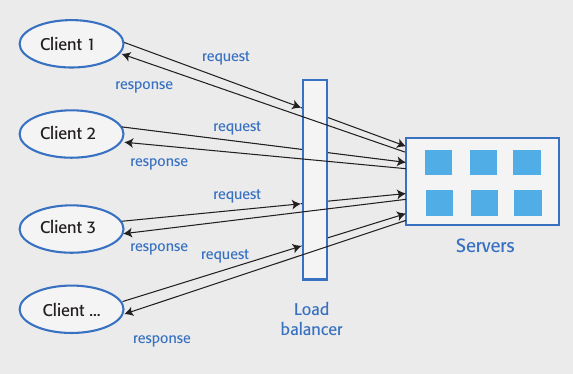
\includegraphics[width=0.7\textwidth]{image29}
	\caption{The orange highlight that concerns may not be always full separated in practice}
	\label{image29}
\end{figure}

In a client-server architecture, a widely used pattern is \textbf{MVC} or \textbf{Mode-View-Cntroller} that allows to model a decouple system from it's design phase. Each view registers with model so that if model changes, all views can be updated.
 \begin{figure}[h]
	\centering
	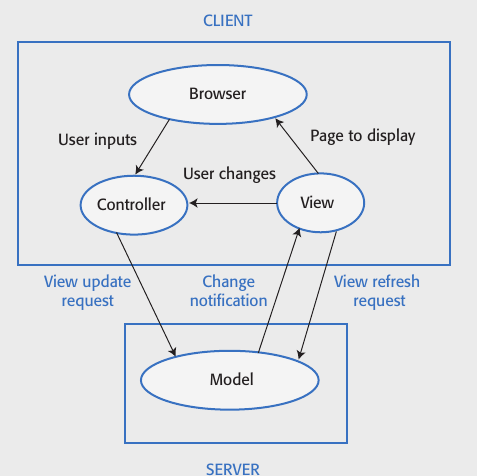
\includegraphics[width=0.7\textwidth]{image30}
	\caption{MVC Model}
	\label{image30}
\end{figure}

\subsection{Client-server communication}
Client-server communication normally uses the HTTP protocol. The client sends a message to the server that includes an instruction such as GET or POST along with the identifier of a resource (usually a URL) on which
that instruction should operate. The message may also include additional information, such as information collected from a form.
HTTP is a text-only protocol so structured data has to be represented as
text. There are two ways of representing this data that are widely used, namely XML and JSON: XML is a markup language with tags used to identify each data item. Also JSON is a simpler representation based on the representation of objects in the Javascript language.

 \begin{figure}[h]
	\centering
	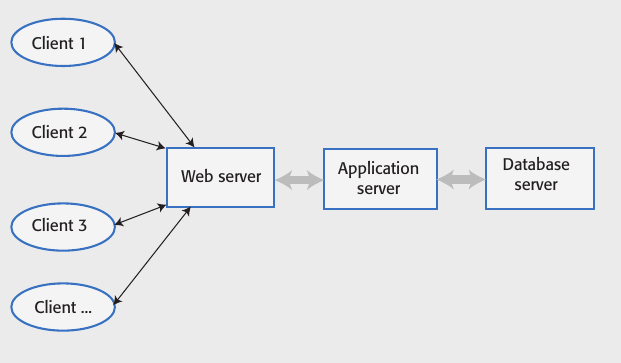
\includegraphics[width=0.7\textwidth]{image31}
	\caption{Multi-tier client-server architecture}
	\label{image31}
\end{figure}

\subsection{SOA - Service-Oriented Architecture}
Services in a service-oriented architecture are stateless components, which means that they can be replicated and can migrate from one computer to another: many servers may be involved in providing services- A service-oriented architecture is usually easier to scale as demand increases and is resilient to failure.
 \begin{figure}[h]
	\centering
	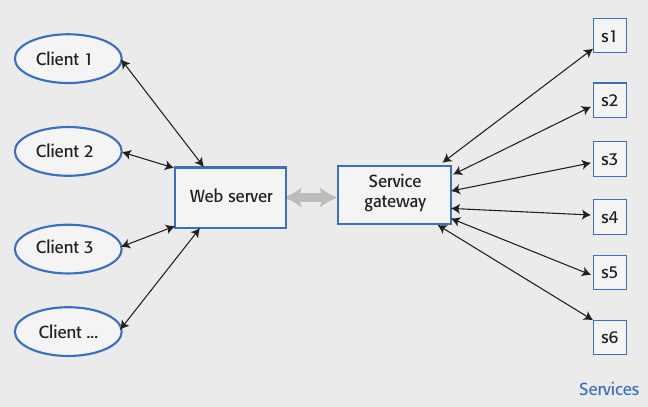
\includegraphics[width=0.7\textwidth]{image32}
	\caption{SOA model}
	\label{image32}
\end{figure}

To \textbf{choose a distribution architecture} we must considerate the following areas:
\begin{itemize}
	\item Data type and data updates: If you are mostly using structured data that may be updated by different system features,
	it is usually best to have a single shared database that provides locking and transaction
	management. If data is distributed across services, you need a way to keep it consistent
	and this adds overhead to your system.
	
	\item Change frequency: If you anticipate that system components will be regularly changed or replaced, then
	isolating these components as separate services simplifies those changes.
	
	\item The system execution platform: If you plan to run your system on the cloud with users accessing it over the Internet, it is usually best to implement it as a service-oriented architecture because scaling the system is simpler.If your product is a business system that runs on local servers, a multi-tier architecture may be more appropriate.
\end{itemize}

\section{Technology choices}
The technology choices must concentrate on component like \textit{database, platform, server, open source software} and \textit{development tools}. These choices affect and constrain the overall system architecture and it's difficult to change them during the development phase.

\subsection{Database}
There are two kinds of database that are now commonly used: Relational databases, where the data is organised into structured tables and NoSQL databases, in which the data has a more flexible, user-defined
organization.
Relational databases, such as MySQL, are particularly suitable for situations where you need transaction management and the data structures are predictable and fairly simple.
NoSQL databases, such as MongoDB, are more flexible and potentially more efficient than relational databases for data analysis. NoSQL databases allow data to be organized hierarchically rather than as flat
tables and this allows for more efficient concurrent processing of ‘big data’.

\subsection{Delivery platform}
Delivery can be as a web-based or a mobile product or both. On Mobile platform we can encounter issues like intermittent connectivity so you must be able to provide a limited service without network connectivity.
Another issue can be the lack of processing power so you need to minimize computationally-intensive operations or the power management issue in which the life's battery is limited so you should try to minimize
the power used by your application.

To deal with these differences, you usually need separate browser-based and mobile versions of your product front-end. You may need a completely different decomposition architecture in these different
versions to ensure that performance and other characteristics are maintained.

\subsection{Server}
 A key decision that you have to make is whether to design your system to run on customer servers or to run on the cloud. For consumer products that are not simply mobile apps I think it almost always makes sense to develop for the cloud but business products, it is a more difficult decision.

Some businesses are concerned about cloud security and prefer to run their systems on in-house servers. They may have a predictable pattern of system usage so there is less need to design your system to cope with large changes in demand. An important choice you have to make if you are running your software
on the cloud is which cloud provider to use to avoid the \textbf{vendor lock-in} problem. 

\subsection{Development technology}
Development technologies (e.g. mobile development toolkit, web application framework) influence the architecture of your product (\textit{e.g. many web development frameworks assume use of model-view-controller architectural pattern}). Also, the development technology that you use may indirectly
influence the architecture of your product (\textit{e.g. if your team is used to relational databases then switching to a non-relational one can be a slow process}).
\skippingparagraph
\section{EIP - Enterprise Integration Patterns}
The enterprise applications distributed around the world are composed by heterogeneous services: some of them are sources of data, some are storing services or computing services. Under a develpment view, on some services we can act by modifying the structure but, usually, we don't have much control on some services (\textit{like a MongoDB instance}).  This implies that in a software ecosystem we can have different data types with different representations also for the data within the same context.
So, enterprise applications are \textbf{compelx distributed multi-service applications} whose services must play together, being them suitably integrated

The \textbf{architectural} question is how to integrate multiple different services to realize enterprise applications that are \textit{coherent (by understanding each other), extensibile, maintanable} and \textit{reasonably simple to understand}.
This is the key idea behind the \textbf{enterprise application integration patterns} that allows to manage the complexity behind every system, tolerate the changes and be a unified model by introducing \textbf{pattern based} methods.

\section{Patterns}
A \textbf{pattern} is an high-level abstraction of accepted, reusable solutions to recurring problems. Typically, patterns are given in terms of the following schema:
	\begin{itemize}
		\item problem statement: including involved software components
		\item context: including involved actors
		\item forces: clarifying the problem rationale and importance
		\item solution: given abstractly, and independent of its actual implementations
	\end{itemize}
When facing a problem, considering existing patterns that are applicable to solve such problem saves us from re-inventing the wheel and making the same mistakes as others.
 \begin{figure}[h]
	\centering
	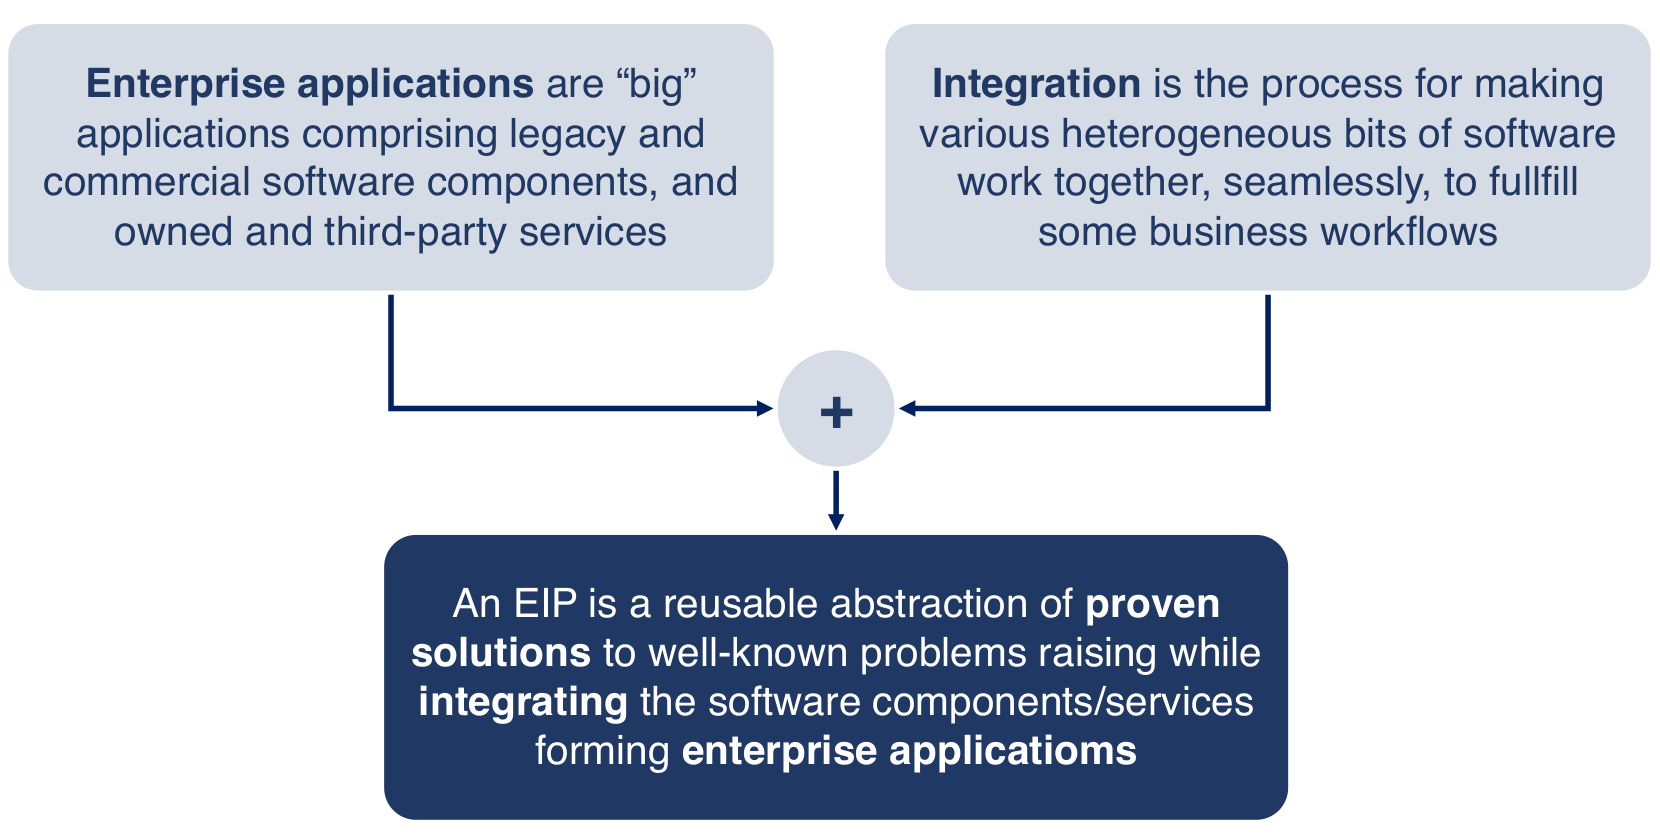
\includegraphics[width=0.7\textwidth]{image33}
	\caption{EIPs context model}
	\label{image33}
\end{figure}

EIPs allows different paradigms along the systems componenets: there are 65 integration patterns described in \textit{Gregor Hohpe, Bobby Woolf, \textbf{Enterprise Integration Patterns: Designing, Building, and Deploying Messaging Solutions}}, describing how each component can be integrated in relation with it's functional and non-functional requirements. The schema in \ref{image34} list a portion of them. 
 \begin{figure}[h]
	\centering
	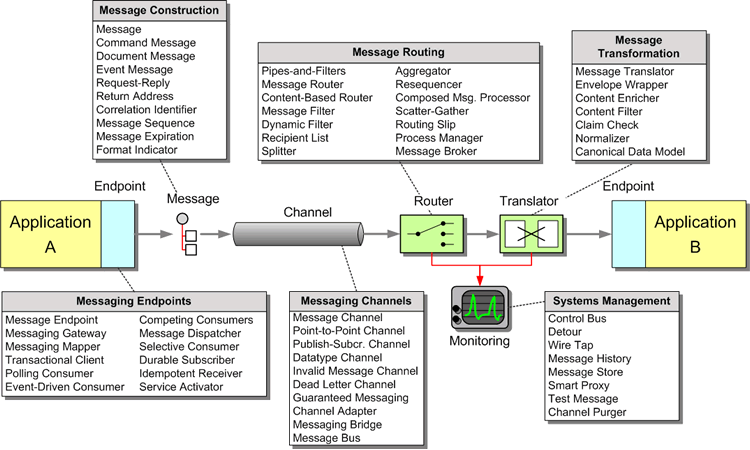
\includegraphics[width=0.7\textwidth]{image34}
	\caption{EIPs component based patterns}
	\label{image34}
\end{figure}

\subsection{Messages}
All systems need to communicate each other: internally, the same happens for componenets and sub-systems. This evolves around a \textbf{message} that is a discrete piece of data sent from a service to another. It's typically structured into header (\textit{considered as metadata}) and body (\textit{the real data payload}). We can distinguish three types of messages according to picture \ref{image35}.
 \begin{figure}[h]
	\centering
	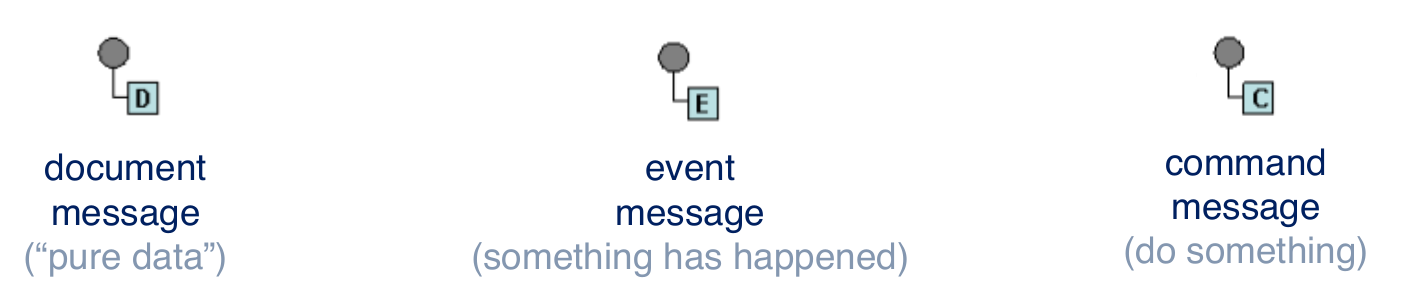
\includegraphics[width=0.7\textwidth]{image35}
	\caption{First message content classification}
	\label{image35}
\end{figure}

The message-based communication allows to create services that are \textit{loosely coupled} by using a simple exchange pattern (\textit{a one-way pattern between sender and receiver}). The messages's format and metadata can also be independent of the integrated services. The communication is realized via \textbf{channels}: it's an abstraction for components sending messages from a source to destination. Under the hood, they can be implemented in many different ways (\textit{RPC, HTTP, TCP, etc}). In \ref{image36} an abstracted schema.
  \begin{figure}[h]
 	\centering
 	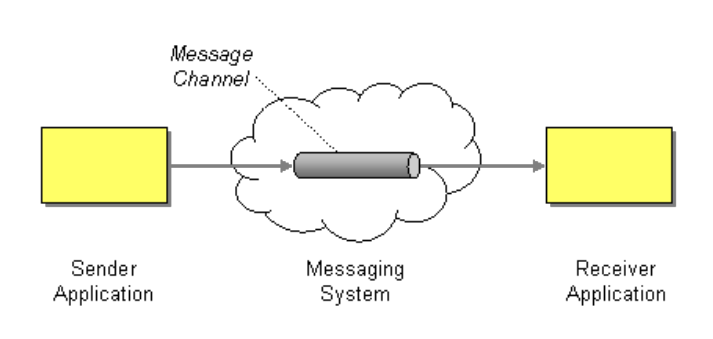
\includegraphics[width=0.7\textwidth]{image36}
 	\caption{One-way communication with channel}
 	\label{image36}
 \end{figure}
The channels are \textbf{one-way} so communications are natively \textbf{asynchronous}: to realize a synchronous communication we need to use two different (\textit{"parallel"}) channels. 

We can also distinguish in different types of channels: a \textbf{point-to-point} (\ref{image37}) channel and a \textbf{publish-subscribe} (\ref{image38}) one. The first one allow to ensure that only one receiver will receive a particular message. The messages's order is not stricly imposed and can be dependent upon the specific functional features to be implemented.
The second one differently allows to deliver a copy of incoming messages to each receiver. 

\begin{figure}
	\centering
	\begin{subfigure}{.5\textwidth}
		\centering
		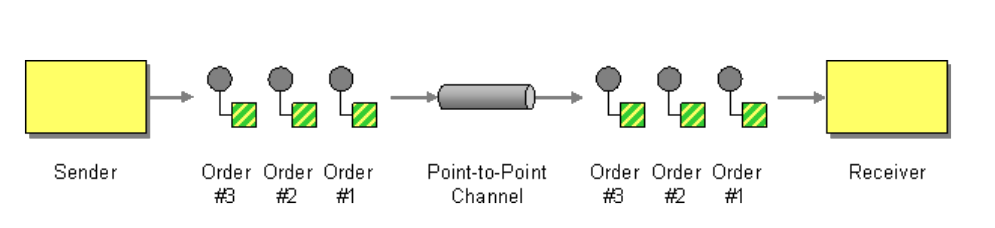
\includegraphics[width=.9\linewidth]{image37}
		\caption{Point-topoint}
		\label{image37}
	\end{subfigure}%
	\begin{subfigure}{.5\textwidth}
		\centering
		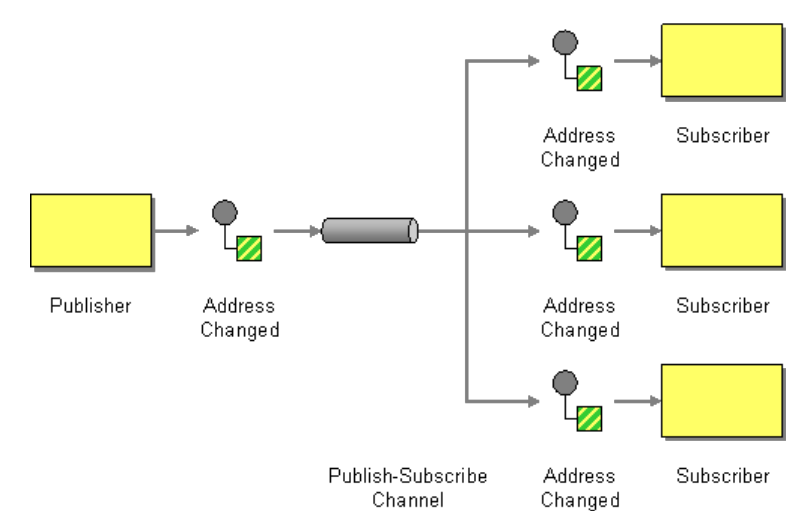
\includegraphics[width=.9\linewidth]{image38}
		\caption{Publish-subscribe}
		\label{image38}
	\end{subfigure}
	\caption{Channel types}
	\label{image38a}
\end{figure}

\subsection{Binding messages}
Application services are typically independent of the messaging systems: they needs some \textit{binding} components to abstract the specific details of the messaging system between the two services.
In \ref{image39} we present an \textbf{adapter} that enable application-specific data to be sent to channels. Typically it's used for the business logic layer/data manipulation. 
In \ref{image40} we present a \textbf{message endpoint} that enable application services to send/receive messages to/from channels. 


\begin{figure}
	\centering
	\begin{subfigure}{.5\textwidth}
		\centering
		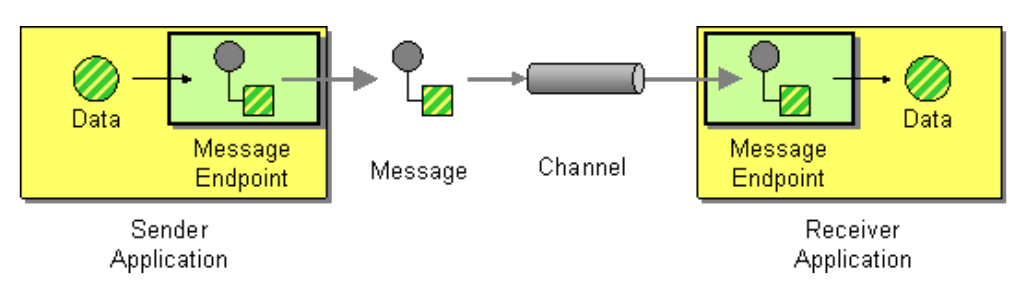
\includegraphics[width=.9\linewidth]{image40}
		\caption{Point-topoint}
		\label{image39}
	\end{subfigure}%
	\begin{subfigure}{.5\textwidth}
		\centering
		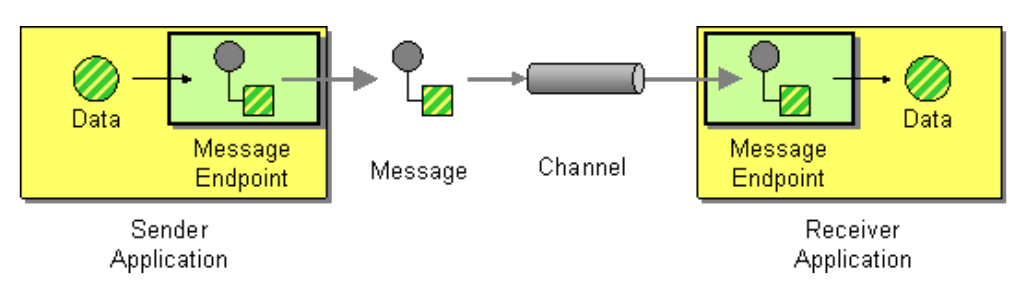
\includegraphics[width=.9\linewidth]{image40}
		\caption{Publish-subscribe}
		\label{image40}
	\end{subfigure}
	\caption{Binding components}
	\label{image40a}
\end{figure}

A simple integration is represented by using message endpoints and channels: the message endpoints is used by services to send/receive messages, channels allows to transport messages from a service to another.

\subsection{Message transformation}
Sending and receiving services may expect different data types or formats both for the header and body. So we introduce a \textbf{message translator} to be able to decode the correct/expected message format. The schema in \ref{image41} describe the message transformation by convert a message from a \textit{red-one} type to a \textit{green} one.
  \begin{figure}[h]
	\centering
	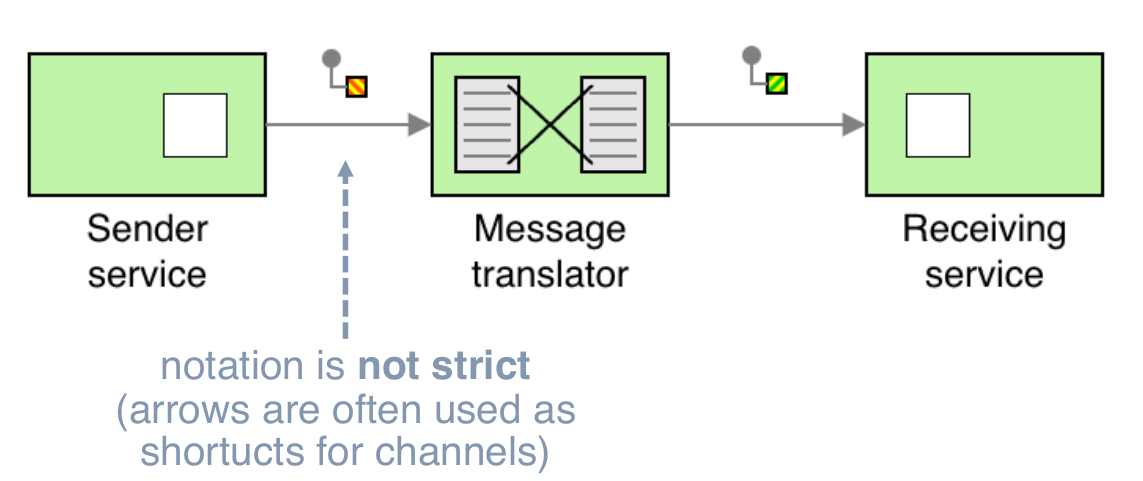
\includegraphics[width=0.7\textwidth]{image41}
	\caption{Message translator pattern}
	\label{image41}
\end{figure}

Message translators enable transforming messages, but other other steps may need to take place
For instance, we need to reasonate about:
\begin{itemize}
	\item How to route messages to different/multiple endpoints? (\textit{e.g. to allow data differentiate computation})
	\item How to split messages? (\textit{e.g in case of a large JSON body})
	\item How to aggregate messages?
\end{itemize}

\subsection{Pipes and filters}
The pipes and filters architectural style (plus other EIPs) enable structuring the more complex integration needed by enterprise applications: messages pass through multiple steps/components processing it (the filters). These components send message down the channels (pipes) they are connected to. 
Note that pipes and filters all deal with the same message/channel abstraction, and can be composed flexibly depending on the circumstances. 

Let's see a navigated example called \textbf{Loan Broker} example in \ref{image42}. The incoming requests are indicated by the green messages, the responses are the red messages: we'll introduce the unknown components marked with \textit{?} following. 
  \begin{figure}[h]
	\centering
	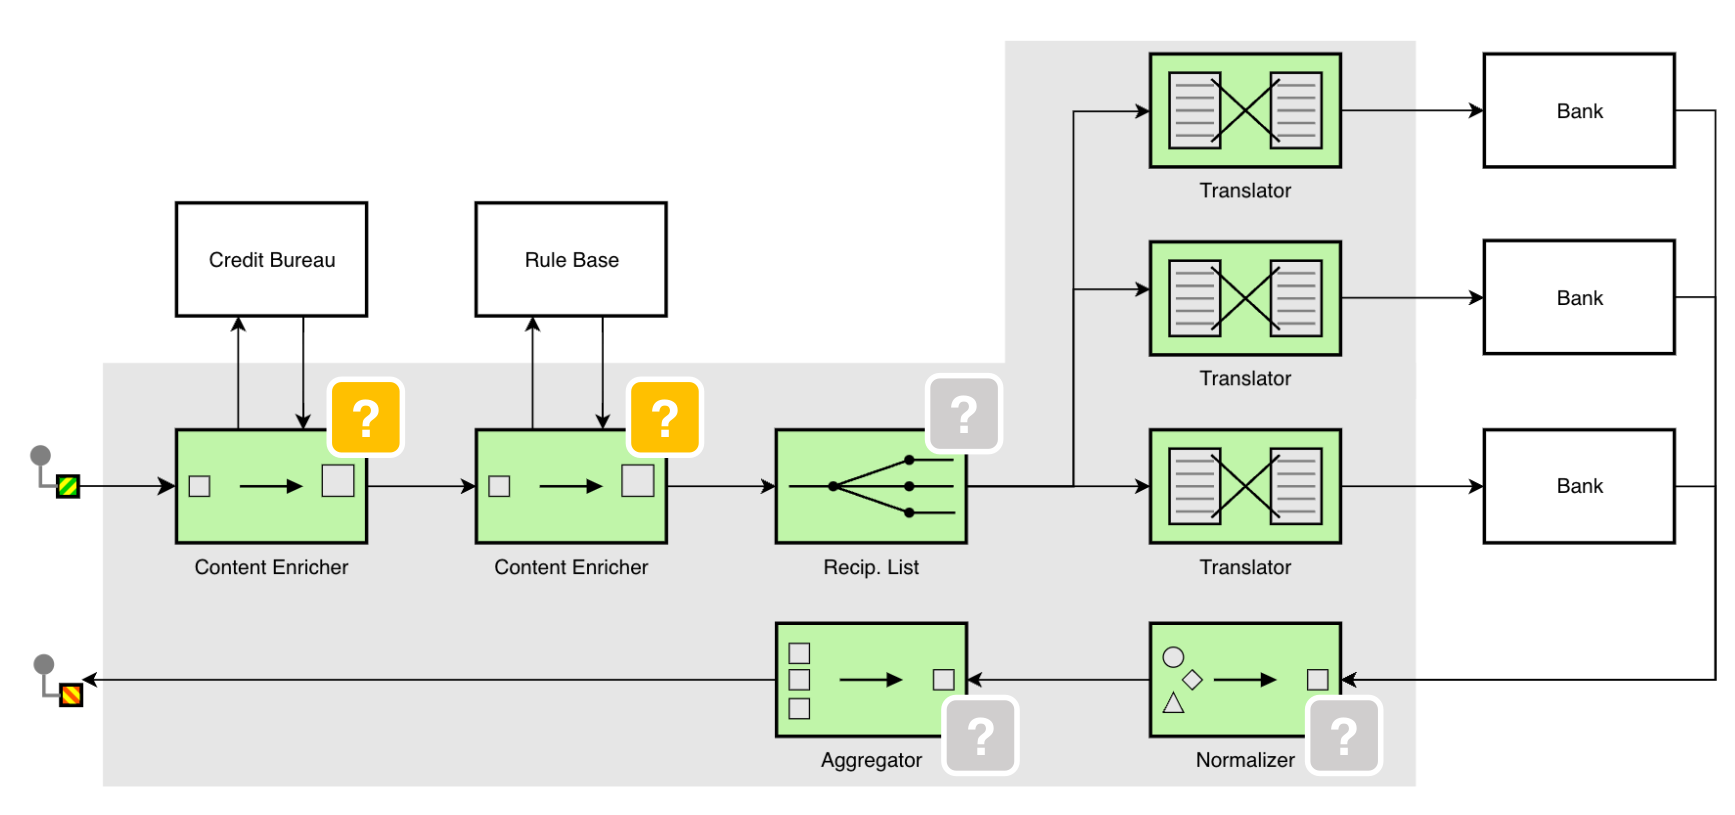
\includegraphics[width=0.9\textwidth]{image42}
	\caption{Loan Broker example schema}
	\label{image42}
\end{figure}

The first component along the path is the \textbf{component enricher} (\ref{image43}): when sending messages from a service to another, the target service may require more information than the source service can provide. The content enricher uses information inside the incoming message (\textit{e.g. key fields}) to retrieve data from an external source. The retrieved data is appended to messages, typically by extending the header/trailer of the message or by encapsulating it inside another message representation. Original information may be carried over or no longer needed, depending on the specific needs of the receiving service.
  \begin{figure}[h]
	\centering
	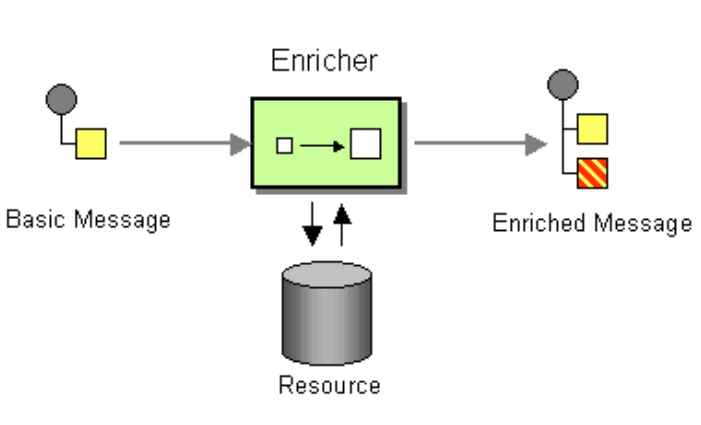
\includegraphics[width=0.4\textwidth]{image43}
	\caption{Loan Broker example schema}
	\label{image43}
\end{figure}
Another component is the \textbf{message routing} (\textit{in \ref{image42} the Recipient List}) that allows a form of \textit{dynamic routing} of messages based on some criteria. This component is needed in a context where endpoint can change or flexibility among the semantics of the messages is required. Some criteria on which we can base the routing are \textbf{content-based} in which we can route messages basaed on message type (\textit{in headers}) or message content (\textit{in body}); or \textbf{context-based} that can route messages based on contextual information (\textit{e.g. a level 7 Load Balancer}). Some routing pattern are listed in \ref{image44}.
In general, a message router is connected to multiple channels and contains the logic to decide which channel it should send to.
  \begin{figure}[h]
	\centering
	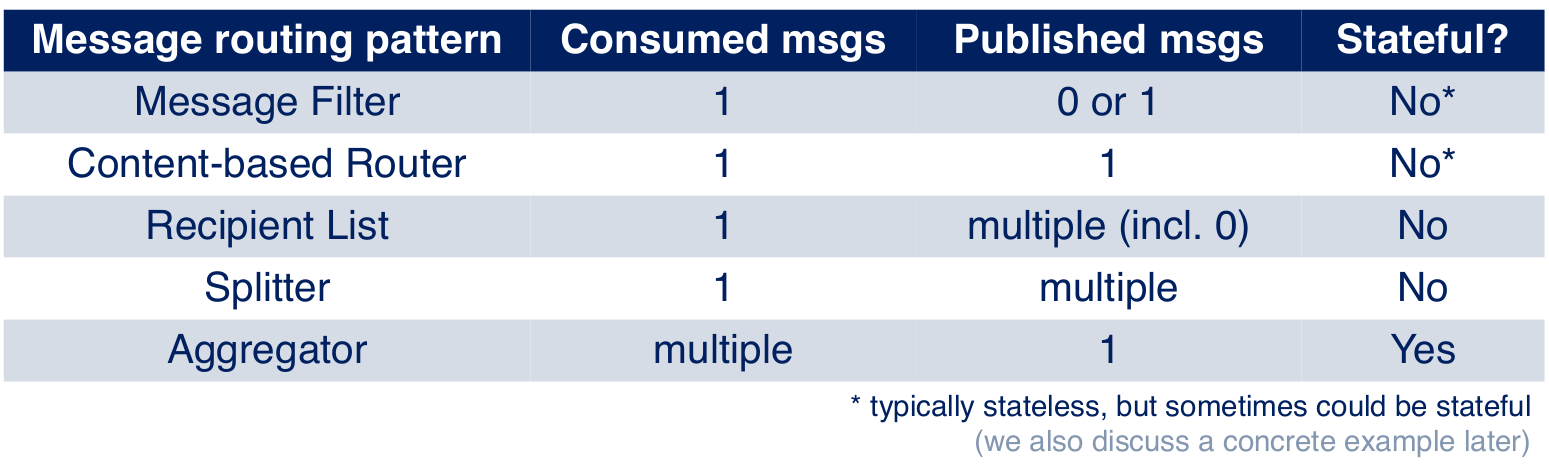
\includegraphics[width=0.7\textwidth]{image44}
	\caption{Routing pattern}
	\label{image44}
\end{figure}

Let's examine the \textbf{message filtering} listed in \ref{image44}: suppose that an enterprise applications sells gadget and widgets, also sending price changes/promtions to large customers. A message filter can eliminate undersired messages froma channel besd ona given criteria, for example if a customer is interested only in the widgets items. 
Given a message passed throught the message filter, we have only one output channel: if a message matches the given criteria, it's routed to the output channel; otherwise is discarded.
A \textbf{recipient list} inspects an incoming message, determines the list of desired recipients and forwards the message to all channels addociated with the recipients in the list, as pictured in \ref{image45}.

\begin{figure}
	\centering
	\begin{subfigure}{.5\textwidth}
		\centering
		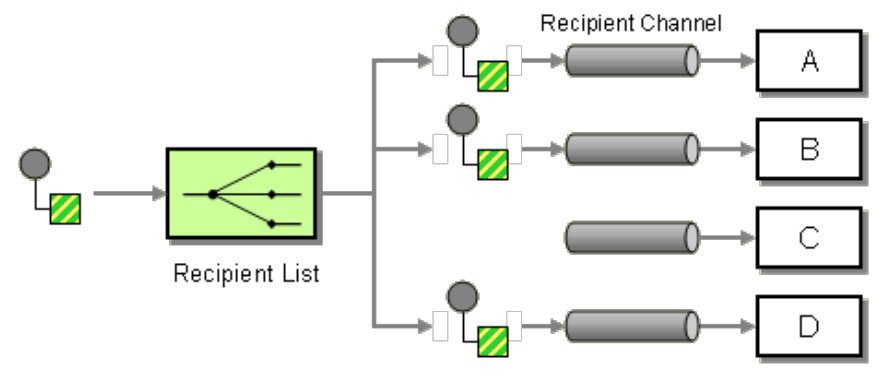
\includegraphics[width=.9\linewidth]{image45}
		\caption{Recipient list pattern}
		\label{image45}
	\end{subfigure}%
	\begin{subfigure}{.5\textwidth}
		\centering
		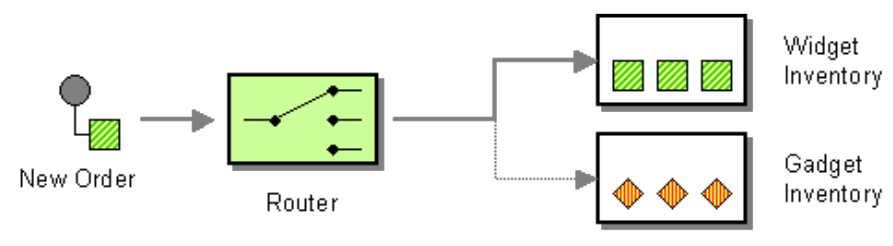
\includegraphics[width=.9\linewidth]{image46}
		\caption{Content-based router}
		\label{image46}
	\end{subfigure}
	
	\label{image46a}
\end{figure}

Following the Load Broker example \ref{image42} we introduce the \textbf{normalizer}: enable translating messages to match a common data format. It can be realized as a composition of other EIPs like a message router routing incoming messages to the most suited translator and a set of \textbf{translator} that transform incoming messages to a common format, as in \ref{image47}.
   \begin{figure}[h]
 	\centering
 	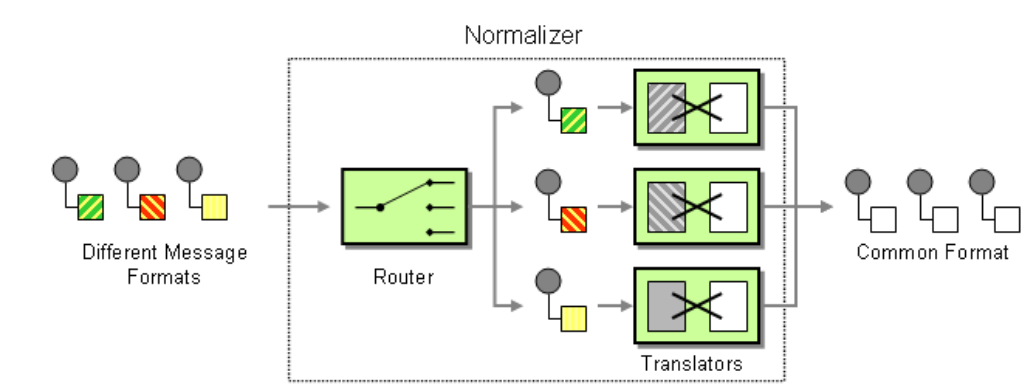
\includegraphics[width=0.5\textwidth]{image47}
 	\caption{Normalizer pattern}
 	\label{image47}
 \end{figure}

The two last component we introduce works in opposite directions. Rather than defining long sequential integrations, some integration steps may go in \textbf{parallel}, for example when sending the loan request to multiple different banks. These are independent processes which can be \textbf{splitted} and executed in parallel: the result of such processes can be \textbf{aggregated} and decisions are made on how to proceed.
A \textbf{splitter} enables breaking out hte composite message into a series of individual messages: each output message contains a different portion of the original message. Also, each output message can be processed differently from others by exploiting content-nased routers to ship them to different processing chains. 
A stateful \textbf{aggregator} enables collecting and storing individual messages until a complete set of related messages has been received: then publishes a single message distilled from the individual messages. The published message can be processed as a whole.  

\begin{figure}
	\centering
	\begin{subfigure}{.5\textwidth}
		\centering
		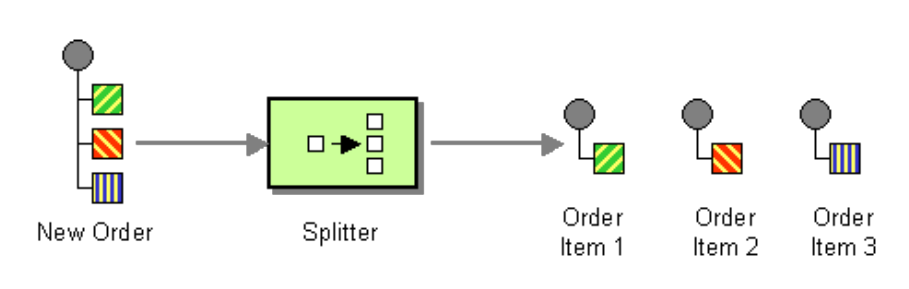
\includegraphics[width=.9\linewidth]{image48}
		\caption{Splitter}
		\label{image48}
	\end{subfigure}%
	\begin{subfigure}{.5\textwidth}
		\centering
		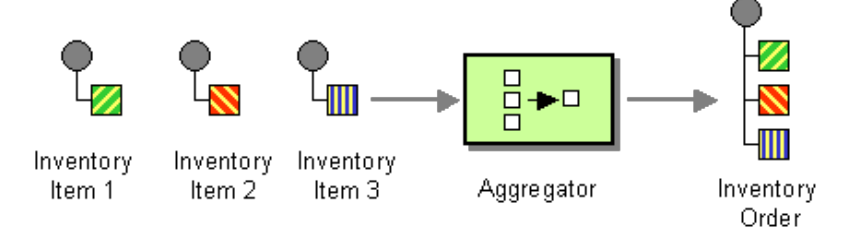
\includegraphics[width=.9\linewidth]{image49}
		\caption{Aggregator}
		\label{image49}
	\end{subfigure}
	
	\label{image49a}
\end{figure}

\chapter{Cloud-based Software}
The cloud is made up of very large number of remote servers that are offered for rent by companies that own these servers: \textbf{Cloud-based servers} are \textit{‘virtual servers’}, which means that they are implementedin software rather than hardware.
You can rent as many servers as you need, run your software on these servers and make them available to your customers: cloud servers can be started up and shut down as demand changes. 
The main advantages, as pictued in \ref{imae50} are:
\begin{itemize}
	\item \textbf{Scalability}: reflects the ability of your software to cope with
	increasingnumbers of users.As the load on your software increases, your software automatically adapts so
	that the system performance and response time is maintained.
	\item \textbf{Elasticity}:  is related to scaleability but also allows for scaling-down as well
	as scaling-up.
	That is, you can monitor the demand on your application and add or remove servers dynamically as the number of users change.
	\item \textbf{Resilience}:  means that you can design your software architecture to
	tolerate server failures. You can make several copies of your software concurrently available. If one of
	these fails, the others continue to provide a service.
	\item \textbf{Cost}:You avoid the initial capital costs of hardware procurement, shifting to a \textit{pay-per-use} paradigm. 
\end{itemize}
   \begin{figure}[h]
	\centering
	\includegraphics[width=0.7\textwidth]{image50}
	\caption{Scalability, resilience and elasticity triangle}
	\label{image50}
\end{figure}

\section{Virtualization: from VMs to containers}
If you are running a cloud-based system with many instances of applications or services, these all use the same operating system, you can use a simpler virtualization technology called ‘containers’.
Using containers accelerates the process of deploying virtual servers on
the cloud: containers are usually megabytes in size whereas VMs are gigabytes and also containers can be started and shut down in a few seconds rather than the few minutes required for a VM.
Containers are an operating system virtualization technology that allows
independent servers to \textbf{share a single operating system}. They are particularly useful for providing isolated application services where each user sees their own version of an application. An abstraction in \ref{image51}.

   \begin{figure}[h]
	\centering
	\includegraphics[width=0.7\textwidth]{image51}
	\caption{VMs VS Containers}
	\label{image51}
\end{figure}

Containers were developed by Google around 2007 but containers became a mainstream technology around 2015.
\textbf{Docker} is one of the most known containerization technology in the world:
\begin{center}
	\textit{
	Docker is a platform that allows us to run applications in an isolated environment \\
	Docker allows us to develop and run portable applications by exploiting containers
}
\end{center}

Containerization technologies came from the past: UNIX \textit{chroot} command provided a simple form of filesystem isolation as the FreeBSD's \textit{jail} utility that extended chroot in 1998 to sandbox processes. In 2005 Google started developing \textbf{cgroups} for Linux kernel and began moving its infrastructure to containers. Only in 2008 the \textit{Linux Containers} (LXC) provided a compelte containerization solution. 
Subsequently evolution happens in 2013 when Docker addded the \textbf{portable images} and \textit{firendly UI}. 

So, to recap, Docker is a container management system that allows users to define the software to be included in a container as a Docker image. It also includes a run-time system that can create and manage
containers using these Docker images.

Docker container system is composed by (\ref{image52}):
\begin{itemize}
	\item \textit{Docker daemon}: This is a process that runs on a host server and is used to setup, start, stop, and monitor containers, as well as building and managing local images.
	\item \textit{Docker client}: This software is used by developers and system managers to define and control containers
	\item \textit{Dockerfiles}: Dockerfiles define runnable applications (images) as a series of setup commands that specify the software to be included in a container. Each container must be
	defined by an associated Dockerfile.
	\item \textit{Image}: A Dockerfile is interpreted to create a Docker image, which is a set of directories
	with the specified software and data installed in the right places. Images are set
	up to be runnable Docker applications.
	\item \textit{Docker Hub}: This is a registry of images that has been created. These may be reused to setup containers or as a starting point for defining new images.
	\item \textit{Containers}: Containers are executing images. An image is loaded into a container and the
	application defined bby the image starts execution. Containers may be moved
	from server to server without modification and replicated across many servers.
	You can make changes to a Docker container (e.g. by modifying files) but you
	then must commit these changes to create a new image and restart the
	container.
\end{itemize}

   \begin{figure}[h]
	\centering
	\includegraphics[width=0.7\textwidth]{image52}
	\caption{Docker container system}
	\label{image52}
\end{figure}
It's noticeable to remember that containers are \textbf{ephimeral} so, to provide persistecy, we need to use \textbf{volumes} that can be mounted to running containers.
\subsection{Docker images}
Docker images are directories that can be archived, shared and run on different Docker hosts. Everything that’s needed to run a software system - binaries, libraries, system tools, etc. is included in the directory. \textbf{Images} are read-only template used to create containers.
A Docker image is a base layer, usually taken from the Docker registry (\textit{which can be a \textbf{private} or \textbf{public} one}), with your own software and data added as a layer on top of this: the layered model means that updating Docker applications is fast and efficient.
Each update to the filesystem is a layer on top of the existing system. To change an application, all you have to do is to ship the changes that you have made to its image, often just a small number of files. Image can also be identified by \textbf{\texttt{repository:tag}} pairs. 
In figure \ref{image53} the commands flow, starting from a \texttt{Dockerfile} to a running container. 

   \begin{figure}[h]
	\centering
	\includegraphics[width=0.7\textwidth]{image53}
	\caption{Docker commands flow}
	\label{image53}
\end{figure}

\subsection{Advantages of Docker}
They solve the problem of software dependencies. You don’t have to worry about the libraries and other software on the application server being different from those on your development server.

Instead of shipping your product as stand-alone software, you can ship a container that includes all of the support software that your product needs.
They provide a mechanism for software portability across different clouds. Docker containers can run on any system or cloud provider where the Docker daemon is available.
They provide an efficient mechanism for implementing software services and so support the development of service-oriented architectures.
They simplify the adoption of DevOps: this is an approach to software support where the same team are responsible for both developing and supporting operational software.

\subsection{Docker Compose}

Compose is a tool for defining and running multi-container Docker applications. With Compose, you use a YAML file to configure your application’s services. Then, with a single command, you create and start all the services from your configuration.

Compose works in all environments: production, staging, development, testing, as well as CI workflows. It also has commands for managing the whole lifecycle of your application:
\begin{itemize}
	\item Start, stop, and rebuild services
	\item View the status of running services
	\item Stream the log output of running services
	\item Run a one-off command on a service
\end{itemize}


We briefly present some useful commands to remember:
\begin{itemize}
	\item \texttt{`docker-compose up`} is the command to deploy a Compose app. It expects the Compose file to be called docker-compose.yml or docker-compose.yaml, but you can specify a custom filename with the -f flag.It’s common to start the app in the background with the -d flag.
	\item \texttt{ `docker-compose stop`} will stop all of the containers in a Compose app without deleting them from thesystem. THe app can be easily restarted with docker-compose restart.
	\item \texttt{`docker-compose rm`} will delete a stopped Compose app. It will delete containers and networks, but it will not delete volumes and images.
	\item \texttt{`docker-compose restart`} will restart a Compose app that has been stopped with docker-compose stop.If you have made changes to your Compose app since stopping it, these changes will not appear in the restarted app. You will need to re-deploy the app to get the changes.
	\item \texttt{`docker-compose ps`} will list the container in the Compose app. It shows current state, the command that  one is running, and network ports.
	\item \texttt{`docker-compose down`} will stop and delete a running Compose app. It deletes containers and networks, but not volumes and images
\end{itemize}
Extensive example and documentation can be found here:
\begin{itemize}
	\item \href{https://learn.microsoft.com/en-gb/dotnet/architecture/microservices/multi-container-microservice-net-applications/multi-container-applications-docker-compose}{Microsoft -  Defining your multi-container application with docker-compose.yml}
	\item \href{https://docs.docker.com/compose/features-uses/}{Docker Compose Documentation - Key features and use cases}
\end{itemize}

\section{Everything as a service}
The idea of a service that is rented rather than owned is fundamental to
cloud computing:
\begin{itemize}
	\item Infrastructure as a service (IaaS):
	Cloud providers offer different kinds of infrastructure service such as a compute
	service, a network service and a storage service that you can use to implement
	virtual servers. (\textit{e.g. salesforce.com})
	\item Platform as a service (PaaS):
	This is an intermediate level where you use libraries and frameworks provided by
	the cloud provider to implement your software. These provide access to a range of
	functions, including SQL and NoSQL databases. (\textit{e.g. Heroku, Azure, GAE})
	\item Software as a service (SaaS): 
	Your software product runs on the cloud and is accessed by users through a web
	browser or mobile app. (\textit{EC2, S3})
\end{itemize}

\subsection{SaaS - Software as a Service}
Software products were initially installed on customers’ computers: customers had to configure software, deal with software updates and product company had to maintain different product versions.
SaaS differently allows to deliver product as a service in which customers do not have to install software, they pay a subscription and access product from remote. 

\textbf{Benefits} of SaaS for product providers are:
\begin{itemize}
	\item \textit{Cash flow}: with a regular cash flow customers pay periodic subscription or pay-per-usage
	
	\item \textit{Update management}: You control product updates, customers receive update at same time so no need of simulateneously maintaining several versions. This allows to reduce costs
	
	\item \textit{Continous deployment}:You can deploy new software versions as soon as changes have been made and tested
	
	\item \textit{Payment flexibility}:Different payment options can attract wider range of customers
	e.g. small companies or individuals can avoid paying large upfront software costs
	
	\item \textit{Try before you buy}:You can make early free/low-cost product available and get customer feedback
	
	\item \textit{Data collection}:You can easily collect data on product usage and customers
	
\end{itemize}

Altought there are some cons for customers like:
\begin{itemize}
	\item Privacy regulation conformance: e.g. EU countries have strict laws on storage of personal info
	\item Security concerns: Customers may not want to pass data control to external provider
	\item Network constraints: Can limit response time when much data transfer
	\item Data exchange: Can be difficult if cloud does not provide suitable API
	\item Loss of control over updates
	\item Service updates
\end{itemize}
Some issues whine designing for a SaaS product are:
\begin{itemize}
	\item Local vs remote processing: some featues can be executed only locally: this can reduce network traffic, increasing response speed but can also increase consumption for battery-powered devices
	\item Authentication: product own authentication system vs. federated authentication vs. Third-part authentication (\textit{Google, Linkedin, etc}).
	\item Information leakage: security risks with multiple users from multiple organizations
	\item Multi-tenant vs multi-instance database management: single repository vs separate copies of system and database
\end{itemize}
\subsection{Multi-tenant systems}
 A multi-tenant database is partitioned so that customer companies have
their own space and can store and access their own data. There is a single database schema, defined by the SaaS provider, that is shared
by all of the system’s users: items in the database are tagged with a tenant identifier, representing a
company that has stored data in the system. The database access software
uses this tenant identifier to provide ‘logical isolation’, which means that users
seem to be working with their own database.

Mid-size and large businesses rarely want to use generic multi-tenant software, often prefer a customized version adapted to their own requirements by customizing:
\begin{itemize}
	\item \textit{Authentication}:
	Businesses may want users to authenticate using their business credentials rather
	than the account credentials set up by the software provider. I explain, in Chapter 7,
	how federated authentication makes this possible.
	\item \textit{Branding}:
	Businesses may want a user interface that is branded to reflect their own organisation.
	\item \textit{Business rules}:
	Businesses may want to be able to define their own business rules and workflows that
	apply to their own data.
	\item \textit{Data schemas}:
	Businesses may want to be able to extend the standard data model used in the
	system database to meet their own business needs.
	\item \textit{Access control}:
	Businesses may want to be able to define their own access control model that sets out
	the data that specific users or user groups can access and the allowed operations on
	that data.
\end{itemize}

\textbf{UI configurability} can be implemented by employing user profiles: users asked to select their organization or provide their business email address. Product uses profile information to
create personalized version of interface like generic company name and logo replace
with company’s ones or some features of menus are disabled (as in \ref{image54}).
   \begin{figure}[h]
	\centering
	\includegraphics[width=0.7\textwidth]{image54}
	\caption{User profiles for SaaS access}
	\label{image54}
\end{figure}

To \textbf{adapt the DB schema} in a multi-tenant system we can evaluate two different solution:
\begin{enumerate}
	\item \textit{Solution 1}: You add some extra columns to each database table and define a
	customer profile that maps the column names that the customer wants to
	these extra columns. However it is difficult to know how many extra columns you should include. If you have too few, customers will find that there aren’t enough for what they need to do.
	
	If you cater for customers who need a lot of extra columns, however, you will find
	that most customers don’t use them, so you will have a lot of wasted space in your
	database. Different customers are likely to need different types of columns. Picture \ref{image55}.
	
	
	\item \textit{Solution 2}:  allow customers to
	add any number of additional fields and to define the names, types and
	values of these fields. The names and types of these values are held in a separate table,
	accessed using the tenant identifier.Unfortunately, using tables in this way adds complexity to the database
	management software.
	Extra tables must be managed and information from them integrated into the
	database.  Picture \ref{image56}
	
	
\end{enumerate}

\begin{figure}
	\centering
	\begin{subfigure}{.5\textwidth}
		\centering
		\includegraphics[width=.9\linewidth]{image55}
		\caption{Solution 1}
		\label{image55}
	\end{subfigure}%
	\begin{subfigure}{.5\textwidth}
		\centering
		\includegraphics[width=.9\linewidth]{image56}
		\caption{Solution 2}
		\label{image56}
	\end{subfigure}
	
	\label{image56a}
\end{figure}

Information from all customers is stored in the same database in a multi-tenant system so a software bug or an attack could lead to the data of some or all customers being exposed to others. \textbf{Key security issues} are multilevel access control and encryption. 

\textbf{Multilevel access control} means that access to data must be controlled at both
the organizational level and the individual level. You need to have organizational level access control to ensure that any
database operations only act on that organization’s data. The individual user
accessing the data should also have their own access permissions.

\textbf{Encryption} of data in a multitenant database reassures corporate users
that their data cannot be viewed by people from other companies if some
kind of system failure occurs.


\textbf{Multi-instance} systems are SaaS systems where each customer has its own
system that is adapted to its needs, including its own database and security
controls. Multi-instance, cloud-based systems are conceptually simpler than multi-tenant
systems and avoid security concerns such as data leakage from one organization
to another.There are two types of multi-instance system:
\begin{itemize}
	\item \textbf{VM-based} multi-instance systems are multi-instance systems where the software
	instance and database for each customer runs in its own virtual machine. All users from
	the same customer may access the shared system database.
	
	\item \textit{Container-based} multi-instance systems* These are multi-instance systems where each
	user has an isolated version of the software and database running in a set of containers.
\end{itemize}

Some pros of multi-instance databases are:
\begin{itemize}
	\item Flexibility:
	Each instance of the software can be tailored and adapted to a customer’s needs.
	Customers may use completely different database schemas and it is
	straightforward to transfer data from a customer database to the product database.
	\item Security:
	Each customer has their own database so there is no possibility of data leakage
	from one customer to another.
	\item Scaleability:
	Instances of the system can be scaled according to the needs of individual
	customers. For example, some customers may require more powerful servers than
	others.
	\item Resilience:
	If a software failure occurs, this will probably only affect a single customers. Other
	customers can continue working as normal.
	
\end{itemize}

Also, the disadvantages are:
\begin{itemize}
	\item Cost:
	It is more expensive to use multi-instance systems because of the costs of
	renting many VMs in the cloud and the costs of managing multiple systems.
	Because of the slow startup time, VMs may have to be rented and kept running
	continuously, even if there is very little demand for the service.

	
	\item Update management:
	It is more complex to manage updates to the software because many instances
	have to be updated. This is particularly problematic where individual instances
	have been tailored to the needs of specific customers.
	
\end{itemize}

\subsection{Architectural decisions}
   \begin{figure}[h]
	\centering
	\includegraphics[width=0.7\textwidth]{image57}
	\caption{Architectural decision diagram}
	\label{image57}
\end{figure}

First, we analyze \textbf{DB organization}. there are three possible ways of providing a customer database in a cloud-based system:
\begin{enumerate}
	\item  As a multi-tenant system,
	shared by all customers for
	your product. This may be
	hosted in the cloud using large,
	powerful servers.
	\item As a multi-instance system,
	with each customer database
	running on its own virtual
	machine.
	\item As a multi-instance system,
	with each database running in
	its own container. The
	customer database may be
	distributed over several
	containers.
\end{enumerate}
The factors to observe regarding the choice are:
\begin{itemize}
	\item Target customers: 
	Do customers require different database schemas and database personalization? Do customers
	have security concerns about database sharing? If so, use a multi-instance database.
	\item Transaction requirements:
	Is it critical that your products support ACID transactions where the data is guaranteed to be
	consistent at all times? If so, use a multi-tenant database or a VM-based multi-instance database.
	\item Database size and connectivity:
	How large is the typical database used by customers? How many relationships are there between
	database items? A multi-tenant model is usually best for very large databases as you can focus
	effort on optimizing performance.
	\item Database interoperability:
	Will customers wish to transfer information from existing databases? What are the differences in
	schemas between these and a possible multitenant database? What software support will they
	expect to do the data transfer? If customers have many different schemas, a multi-instance
	database should be used.
	\item System structure:
	Are you using a service-oriented architecture for your system? Can customer databases be split
	into a set of individual service databases? If so, use containerized, multi-instance databases.
\end{itemize}
Different types of customers have different expectations about
software products. Some examples are:
\begin{itemize}
	\item Consumers or small businesses do not expect branding and personalization, local
	authentication system, or varying individual permissions → You can use a multi-tenant
	database with a single schema
	\item Large companies are more likely to want a database adapted to their needs → Possible to
	some extent with a multi-tenant system, easier with a multi-instance database
	\item For products in which database has to consistent at all times (e.g. finance) → You need a
	transaction-based system: either a multi-tenant database or a database per customer
	running on a virtual machine (with all users from each customer sharing the VM-based
	database)
\end{itemize}

\subsection{Scalability}
The scaleability of a system reflects its ability to adapt automatically to
changes in the load on that system.
You achieve scaleability in a system by making it possible to add new
virtual servers (scaling-out) or increase the power of a system server
(scaling-up) in response to increasing load.

In cloud-based systems, scaling-out rather than scaling-up is the normal
approach used. Your software has to be organized so that individual software
components can be replicated and run in parallel. Also you need load-balancing mechanisms to direct requests to different
instances of the components (e.g. with PaaS). 

\subsection{Resilience}
The resilience of a system reflects its ability to continue to deliver critical
services in the event of system failure or malicious system use. To achieve resilience, you need to be able to restart your software quickly after a hardware or software failure.

Resilience relies on redundancy: the first behaviour is called \textbf{"hot standby"} in which the replicas of the software and data are maintained in different locations. Database updates are mirrored so that the standby database is a working copy of the operational database. A system monitor continually checks the system status. It can switch to the
standby system automatically if the operational system fails.

A second behaviour is knowed as \textbf{"cool standby"} in which you should use redundant virtual servers that are not hosted on the same physical computer and locate servers in different locations.
Ideally, these servers should be located in different data centers: if a physical server fails or if there is a wider data center failure, then operation can be switched automatically to the software copies elsewhere.

\subsection{Software structure}

An object-oriented approach to software engineering has been that been
extensively used for the development of client-server systems built
around a shared database.
The system itself is, logically, a \textbf{monolithic system} with distribution across multiple servers running large software components. The traditional multi-tier client server architecture is based on this distributed system model.

The alternative to a monolithic approach to software organization is a service-oriented approach where the system is decomposed into \textbf{fine-grain, stateless services}: because it is stateless, each service is independent and can be replicated,distributed and migrated from one server to another. The service-oriented approach is particularly suitable for cloud-based software with services deployed in containers.

\textbf{Cloud platforms} include general-purpose clouds such as Amazon Web
Services or lesser known platforms oriented around a specific
application, such as the SAP Cloud Platform. There are also smaller
national providers that provide more limited services but who may be
more willing to adapt their services to the needs of different customers.

There is no ‘best’ platform and you should choose a cloud provider
based on your background and experience, the type of product that you
are developing and the expectations of your customers.
You need to consider both \textbf{technical issues} (\ref{image58}) and \textbf{business issues} (\ref{image59}) when
choosing a cloud platform for your product.

\begin{figure}
	\centering
	\begin{subfigure}{.5\textwidth}
		\centering
		\includegraphics[width=.9\linewidth]{image58}
		\caption{Technical issues}
		\label{image58}
	\end{subfigure}%
	\begin{subfigure}{.5\textwidth}
		\centering
		\includegraphics[width=.9\linewidth]{image59}
		\caption{Business issues}
		\label{image59}
	\end{subfigure}
	
	\label{image59a}
\end{figure}

\section{Kubernetes}
K8s manages the entire lifecycle of individual containers, spinning up and shutting down resources as needed:if a container shuts down unexpectedly, K8s reacts by launching another container in its place.
K8s provides a mechanism for applications to communicate with each other even as underlying individual containers are created and destroyed. Given a set of container workloads to run and a set of machines on a cluster, the container orchestrator examines each container and determines the optimal machine to schedule that workload .

Kubernetes is like any other cluster – a bunch of nodes and a control plane. The control plane exposes an API, has a scheduler for assigning work to nodes, and state is recorded in a persistent store. Nodes are where application services run.
It can be useful to think of the control plane as the brains of the cluster, and the nodes as the muscle. In this analogy, the control plane is the brains because it implements all of the important features such as auto-scaling and zero-downtime rolling updates. The nodes are the muscle because they do the every-day hard work of
executing application code.

Orchestrator is just a fancy word for a system that takes care of deploying and managing applications. 

To make this happen, you start out with an app, package it up and give it to the cluster (Kubernetes). The cluster is made up of one or more \textbf{masters} and a \textbf{bunch of nodes}.
The masters, sometimes called heads or head nodes, are in-charge of the cluster. This means they make the scheduling decisions, perform monitoring, implement changes, respond to events, and more. For these reasons, we often refer to the masters as the \textbf{control plane}. 

The nodes are where application services run, and we sometimes call them the data plane. Each node has a reporting line back to the masters, and constantly watches for new work assignments. To run applications on a Kubernetes cluster we follow this simple pattern:
\begin{enumerate}
	\item Write the application as small independent microservices in our favourite languages.
	\item Package each microservice in its own container.
	\item Wrap each container in its own Pod.
	\item Deploy Pods to the cluster via higher-level controllers such as; Deployments, DaemonSets, StatefulSets, CronJobs etc.
\end{enumerate}

\subsection{Master and nodes}
A \textbf{Kubernetes master} is a collection of system services that make up the control plane of the cluster. The simplest setups run all the master services on a single host. However, this is only suitable for labs and test environments. For production environments, multi-master high availability (HA) is a must have. This is why the major cloud providers implement HA masters as part of their hosted Kubernetes platforms such as Azure Kubernetes Service (AKS), AWS Elastic Kubernetes Service (EKS), and Google Kubernetes Engine (GKE).
Generally speaking, running 3 or 5 replicated masters in an HA configuration is recommended.

Let’s take a quick look at the different master services that make up the control plane.
\begin{itemize}
	\item \textbf{API Server}:All communication, between all components, must go through the API server. We’ll get into the detail later in the book, but it’s important to understand that internal
	system components, as well as external user components, all communicate via the same API.
	It exposes a RESTful API that you POST YAML configuration files to over HTTPS. These YAML files, which we sometimes call manifests, contain the desired state of your application. This desired state includes things like; which container image to use, which ports to expose, and how many Pod replicas to run.
	All requests to the API Server are subject to authentication and authorization checks, but once these are done, the config in the YAML file is validated, persisted to the cluster store, and deployed to the cluster.
	
	\item \textbf{Cluster store}:The cluster store is the only stateful part of the control plane, and it persistently stores the entire configuration and state of the cluster. The cluster store is currently based on etcd, a popular distributed database. As it’s the single source of truth for the cluster, you should run between 3-5 etcd replicas for high-availability, and you should provide adequate ways to recover when things go wrong.
	On the topic of availability, etcd prefers consistency over availability. This means that it will not tolerate a split-brain situation and will halt updates to the cluster in order to maintain consistency. However, if etcd becomes unavailable, applications running on the cluster should continue to work, you just won’t be able to
	update anything.
	
	\item \textbf{Control manager}:
	The controller manager implements all of the background control loops that monitor the cluster and respond to events. It’s a controller of controllers, meaning it spawns all of the independent control loops and monitors them. Some of the control loops include; t*he node controller, the endpoints controller, and the replicaset controller.* Each one runs as a background watch-loop that is constantly watching the API Server for changes -– t*he aim of the game is to ensure the current state of the cluster matches the desired state (more on this shortly*).
	The logic implemented by each control loop is effectively this:
	\begin{enumerate}
		\item  Obtain desidered state
		\item Observe current state
		\item Determine differences
		\item Reconcile differences
		
	\end{enumerate}
	
	Each control loop is also extremely specialized and only interested in its own little corner of the Kubernetes cluster. No attempt is made to over-complicate things by implementing awareness of other parts of the system – each control loop takes care of its own business and leaves everything else alone. This is key to the distributed design of Kubernetes and adheres to the Unix philosophy of building complex systems from small specialized parts.
	\item \textbf{Scheduler}: At a high level, the scheduler watches the API server for new work tasks and assigns them to appropriate healthy nodes. Behind the scenes, it implements complex logic that filters out nodes incapable of running the task, and then ranks the nodes that are capable. The ranking system is complex, but the node with the highest-ranking score is selected to run the task.
	
	When identifying nodes that are capable of running a task, the scheduler performs various predicate checks. These include; is the *node tainted*, are there any affinity or anti-affinity rules, is the required network port available on the node, does the node have sufficient free resources etc. Any node incapable of running the task is ignored, and the remaining nodes are ranked according to things such as; does the node already have the required image, how much free resource does the node have, how many tasks is the node already running. Each criterion is worth points, and the node with the most points is selected to run the task.
	
	If the scheduler cannot find a suitable node, the task cannot be scheduled and is marked as pending.
	The scheduler isn’t responsible for running tasks, just picking the nodes a task will run on.
\end{itemize}

\subsubsection{Nodes}
Nodes are the workers of a Kubernetes cluster. At a high-level they do three things:
\begin{enumerate}
	\item Watch the API Server for new work assignments
	\item Execute new work assignments
	\item Report back to the control plane (via the API server)
\end{enumerate}

Let’s look at the three major components of a node:

\begin{itemize}
	\item \textbf{Kubelet}:It’s the main Kubernetes agent, and it runs on every node in the cluster. In fact, it’s common to use the terms node and kubelet interchangeably.
	
	When you join a new node to a cluster, the process installs kubelet onto the node. The kubelet is then responsible for registering the node with the cluster. Registration effectively pools the node’s CPU, memory, and storage into the wider cluster pool.
	One of the main jobs of the kubelet is to watch the API server for new work assignments. Any time it sees one, it executes the task and maintains a reporting channel back to the control plane.
	If a kubelet can’t run a particular task, it reports back to the master and lets the control plane decide what actions to take. 
	
	For example, if a Kubelet cannot execute a task, it is not responsible for finding another node to run it on. It simply reports back to the control plane and the control plane decides what to do.
	
	\item \textbf{Container Runtime Interface (CRI)}:The Kubelet needs a container runtime to perform container-related tasks -– things like pulling images and starting and stopping containers.
	In the early days, Kubernetes had native support for a few container runtimes such as Docker. More recently, it has moved to a plugin model called the Container Runtime Interface (CRI). At a high-level, the CRI masks the internal machinery of Kubernetes and exposes a clean documented interface for 3rd-party container runtimes to plug into.
	
	\item \textbf{Kube-proxy}:
	The last piece of the node puzzle is the kube-proxy. This runs on every node in the cluster and is responsible for local cluster networking. For example, it makes sure each node gets its own unique IP address, and implements local IPTABLES or IPVS rules to handle routing and load-balancing of traffic on the Pod network.
\end{itemize}

There is surely a \textbf{Kubernetes DNS}: the cluster’s DNS service has a static IP address that is hard-coded into every Pod on the cluster, meaning all containers and Pods know how to find it. Every new service is automatically registered with the cluster’s DNS so that all components in the cluster can find every Service by name. Some other components that are registered with the cluster DNS are StatefulSets and the individual Pods that a StatefulSet manages.

\subsection{Declarative model and desired state}

The declarative model and the concept of desired state are at the very heart of Kubernetes. In Kubernetes, the declarative model works like this:

1. Declare the desired state of an application (microservice) in a manifest file
2. POST it to the API server
3. Kubernetes stores it in the cluster store as the application’s desired state
4. Kubernetes implements the desired state on the cluster
5. Kubernetes implements watch loops to make sure the current state of the application doesn’t vary from the desired state

Let’s analyze these steps deeper.
Manifest files are written in simple YAML, and they tell Kubernetes how you want an application to look. This is called the desired state. It includes things such as; which image to use, how many replicas to run, which network ports to listen on, and how to perform updates.

Once you’ve created the manifest, you POST it to the API server. The most common way of doing this is with the \texttt{kubectl} command-line utility. This sends the manifest to the control plane as an HTTP POST, usually on port 443.

Once the request is authenticated and authorized, Kubernetes inspects the manifest, identifies which controller to send it to (e.g. the Deployments controller), and records the config in the cluster store as part of the cluster’s overall desired state. Once this is done, the work gets scheduled on the cluster. This includes the hard work of pulling images, starting containers, building networks, and starting the application’s processes.

Finally, Kubernetes utilizes background reconciliation loops that constantly monitor the state of the cluster. If the current state of the cluster varies from the desired state, Kubernetes will perform whatever tasks are necessary to reconcile the issue.



\begin{figure}[h]
	\centering
	\includegraphics[width=0.9\textwidth]{image-K8S-watch-loop}
	\caption{Watch loop concept}
	\label{k8s-watch-loop}
\end{figure} 
Not only is the declarative model a lot simpler than long scripts with lots of imperative commands, it also enables self-healing, scaling, and lends itself to version control and self-documentation. It does this by telling the cluster how things should look. If they stop looking like this, the cluster notices the discrepancy and does all of the hard work to reconcile the situation.
But the declarative story doesn’t end there – things go wrong, and things change. When they do, the current state of the cluster no longer matches the desired state. As soon as this happens, Kubernetes kicks into action and attempts to bring the two back into harmony.

\subsection{Pods}
In the VMware world, the atomic unit of scheduling is the virtual machine (VM). In the Docker world, it’s the container. Well... in the Kubernetes world, it’s the Pod.
It’s true that Kubernetes runs containerized apps. However, you cannot run a container directly on a Kubernetes cluster – containers must always run inside of Pods.
The very first thing to understand is that the term Pod comes from a pod of whales – in the English language we call a group of whales a pod of whales. As the Docker logo is a whale, it makes sense that we call a group of containers a Pod.
The simplest model is to run a single container per Pod. However, there are advanced use-cases that run multiple containers inside a single Pod. These multi-container Pods are beyond the scope of what we’re discussing here.

At the highest-level, a Pod is a ring-fenced environment to run containers. The Pod itself doesn’t actually run anything, it’s just a sandbox for hosting containers. Keeping it high level, you ring-fence an area of the host OS, build a network stack, create a bunch of kernel namespaces, and run one or more containers in it. 

If you’re running multiple containers in a Pod, they all share the same \textbf{Pod environment}. This includes things like the IPC namespace, shared memory, volumes, network stack and more. As an example, this means that all containers in the same Pod will share the same IP address (the Pod’s IP): If two containers in the same Pod need to talk to each other (container-to-container within the Pod) they can use ports on the Pod’s localhost interface.


\subsection{Deployments}
At a high level, you start with application code. That gets packaged as a container and wrapped in a Pod so it can run on Kubernetes. However, Pods don’t self-heal, they don’t scale, and they don’t allow for easy updates or rollbacks. Deployments do all of these. As a result, you’ll almost always deploy Pods via a Deployment controller.\\
It’s important to know that a single Deployment object can only manage a single \textbf{Pod template}. For example, if you have an application with a Pod template for the web front-end and another Pod template for the catalog service, you’ll need two Deployments. However, as you saw in the previous figure, a Deployment can manage multiple replicas of the same Pod. For example, the figure could be a Deployment that currently manages two replicated web server Pods.

The next thing to know is that Deployments are fully-fledged objects in the Kubernetes API. This means you define them in manifest files that you POST to the API Server. The last thing to note, is that behind-the-scenes, Deployments leverage another object called a ReplicaSet. While it’s best practice that you don’t interact directly with ReplicaSets, it’s important to understand the role they play. Keeping it high-level, Deployments use ReplicaSets to provide self-healing and scaling. 
\begin{figure}[h]
	\centering
	\includegraphics[width=0.7\textwidth]{image-deployment-manage}
	\caption{Deployment encapsulate Pods}
	\label{k8s-deployment-manage-pods}
\end{figure} 
As shown in figure, think of Deployments as managing ReplicaSets, and ReplicaSets as managing Pods. Put them all together, and you’ve got a great way to deploy and manage applications on Kubernetes.

Pods augment containers by allowing \textbf{co-location of containers, sharing of volumes, sharing of memory, simplified networking and so on}. BUt they offer nothing in the way of self-healing and scalability: here \textbf{Deployments} enter the game. 

Deployments augment Pods by adding things these things, that means:
\begin{itemize}
	\item if a Pod managed by a Deployment fails, it will be replaced (self-healing)
	\item if a Pod managed by a Deployment sees increased load, you can easily add more of the same Pod to deal with the load (scaling)
\end{itemize}

Before going any further, it’s critical to understand three concept that are fundamental to everything about K8s:
\begin{itemize}
	\item \textbf{Desired state}: is what you want.
	\item \textbf{Current state}: is what you have; if match with desidered state, everything is fine.
	\item \textbf{Declarative model}: is a way of telling Kubernetes what your desired state is, without having to get into the detail of how to implement it. You leave the how up to Kubernetes.
\end{itemize}

undamental to desired state is the concept of background reconciliation loops or control loops. 

For example, ReplicaSets implement a background reconciliation loop that is constantly checking whether the right number of Pod replicas are present on the cluster. If there aren’t enough, it adds more. If there are too many, it terminates some. \textbf{Kubernetes is constantly making sure that current state matches desired state.}

These very-same reconciliation loops enable scaling. For example, if you POST an updated config that changes replica count from 3 to 5, the new value of 5 will be registered as the application’s new desired state. The next time the ReplicaSet reconciliation loop runs, it will
notice the discrepancy and follow the same process, start the read alert and spinning up two more replicas.

\begin{figure}[h]
	\centering
	\includegraphics[width=0.9\textwidth]{image-deployment-k8s}
	\caption{\texttt{deployment.yaml}}
	\label{k8s-deployment}
\end{figure} 

Right at the very top you specify the API version to use. Assuming that you’re using an up-to-date version of Kubernetes, Deployment objects are in the apps/v1 API group.
Next, the \texttt{.kind} field tells Kubernetes you’re defining a Deployment object. The \texttt{.metadata} section is where we give the Deployment a name and labels.
The \texttt{.spec} section is where most of the action happens. Anything directly below \texttt{.spec} relates to the Pod. Anything nested below \texttt{.spec.template} relates to the Pod template that the Deployment will manage. In this example, the Pod template defines a single container. \texttt{.spec.replicas} tells Kubernetes how may Pod replicas to deploy. \texttt{spec.selector} is a list of labels that Pods must have in order for the Deployment to manage them. 

\subsection{Service}
We’ve just learned that Pods are mortal and can die. However, if they’re managed via \textit{Deployments} or \textit{DaemonSets}, they get replaced when they fail. But replacements come with totally different IP addresses. This also happens when you perform scaling operations – scaling up adds new Pods with new IP addresses, whereas scaling down takes existing Pods away. Events like these cause a lot of \textit{IP churn}.

The point I’m making is that \textbf{Pods are unreliable}, which poses a challenge. Assume you’ve got a microservices app with a bunch of Pods performing video rendering. *How will this work if other parts of the app that need to use the rendering service cannot rely on the rendering Pods being there when they need them?*

This is where Services come in to play. \textbf{Services provide reliable networking for a set of Pods.} Figure shows the uploader microservice talking to the renderer microservice via a Kubernetes Service object. The Kubernetes Service is providing a reliable name and IP, and is load-balancing requests to the two renderer Pods behind it.

Services are fully-fledged objects in the Kubernetes API – just like Pods and Deployments. They have a front-end that consists of a stable DNS name, IP address, and port. On the back-end, they load-balance across a dynamic set of Pods. As Pods come and go, the Service observes this, automatically updates itself, and continues to provide that stable networking endpoint.
The same applies if you scale the number of Pods up or down. New Pods are seamlessly added to the Service and will receive traffic. Terminated Pods are seamlessly removed from the Service and will not receive traffic.

That’s the job of a Service – it’s a stable network abstraction point that provides TCP and UDP load-balancing across a dynamic set of Pods.
As they operate at the TCP and UDP layer, Services do not possess \textit{application intelligence} and cannot provide application-layer host and path routing. For that, you need an \textbf{Ingress}, which understands HTTP and provides host and path-based routing.

\begin{figure}[h]
	\centering
	\includegraphics[width=0.9\textwidth]{image-k8s-service}
	\caption{Service schema}
	\label{image-k8s-service}
\end{figure} 
\begin{figure}[h]
	\centering
	\includegraphics[width=0.9\textwidth]{image-service-yaml}
	\caption{\texttt{service.yaml}}
	\label{image-k8s-service-yaml}
\end{figure} 

In the example files, the Service has a label selector (spec.selector) with a single value \texttt{app=ml-model}. This is the label that the Service is looking for hen it queries the cluster for matching Pods. The Deployment specifies a Pod template with the same \texttt{app=ml-model} label. It’s these two attributes that loosely couple the Service to the Deployment’s Pod.

For some parts of your application (for example, frontends) you may want to expose a Service onto an external IP address, that's outside of your cluster.

Kubernetes \texttt{ServiceTypes} allow you to specify what kind of Service you want.

Type values and their behaviors are:
\begin{itemize}
	\item \textbf{ClusterIP}: Exposes the Service on a cluster-internal IP. Choosing this value makes the Service only reachable from within the cluster. This is the default that is used if you don't explicitly specify a type for a Service.
	\item \textbf{NodePort}: Exposes the Service on each Node's IP at a static port (the NodePort). To make the node port available, Kubernetes sets up a cluster IP address, the same as if you had requested a Service of type: ClusterIP.
	\item \textbf{ExternalName}: Exposes the Service externally using a cloud provider's load balancer.
	\item \textbf{LoadBalancer}: Maps the Service to the contents of the externalName field (e.g. foo.bar.example.com), by returning a CNAME record with its value. No proxying of any kind is set up.
\end{itemize}
 
\subsection{Ingress}
Ingress exposes HTTP and HTTPS routes from outside the cluster to services within the cluster. Traffic routing is controlled by rules defined on the Ingress resource.


\begin{figure}[h]
	\centering
	\includegraphics[width=0.9\textwidth]{image-ingress-k8s}
	\caption{Ingress schema}
	\label{image-k8s-ingress}
\end{figure} 



You must have an Ingress controller to satisfy an Ingress. Only creating an Ingress resource has no effect.
You may need to deploy an Ingress controller such as ingress-nginx. You can choose from a number of Ingress controllers.

Ideally, all Ingress controllers should fit the reference specification. In reality, the various Ingress controllers operate slightly differently.
An Ingress needs \texttt{apiVersion, kind, metadata} and \textit{spec} fields. The name of an Ingress object must be a valid DNS subdomain name. Ingress frequently uses annotations to configure some options depending on the Ingress controller, an example of which is the rewrite-target annotation. Different Ingress controllers support different annotations. Review the documentation for your choice of Ingress controller to learn which annotations are supported.

\begin{figure}[h]
	\centering
	\includegraphics[width=0.9\textwidth]{image-ingress-yaml}
	\caption{\texttt{ingress.yaml}}
	\label{image-k8s-ingress-yaml}
\end{figure} 

The Ingress \texttt{spec} has all the information needed to configure a load balancer or proxy server. Most importantly, it contains a list of rules matched against all incoming requests. Ingress resource only supports rules for directing HTTP(S) traffic.

\subsection{Evaluations}
When should you NOT use K8s?
\begin{itemize}
	\item If you can run your workload on a single machine
	\item If your compute needs are light
	\item If you don't need high availability and can tolerate downtime
	\item If you don't envision making a lot of changes to your deployed services
	\item If you have a monolith and don't plan to break it into microservices
\end{itemize}

In comparison with K8s, \textbf{Docker Swarm} is simpler to install, have a softer learning curve and it's generally preferred in environments where simplicity and fast development are prioritized.



\chapter{Microservices}

A software service is a software component that can be accessed from remote computers over the Internet. Given an input, a service produces a corresponding output, without side effects: the service is accessed through its published interface and all details of the service implementation are hidden. Usually services do not maintain any internal state. State information is either stored in a database or is maintained by the service requestor.

When a service request is made, the state information may be included as part of the request and the updated state information is returned as part of the service result. As there is no local state, services can be dynamically reallocated from one virtual server to another and replicated across several servers.
Some modern web services of 2000s are:
\begin{itemize}
	\item Service-oriented architecture (SOA - 1990s): Independent, stand-alone services, with public interfaces, implemented with different technologies
	\item Web services (early 2000s): use protocol as XML, SOAP, WSDL, plus dozens (!) of other standards. Web services exchanging large and complex XML data that augment message management overhead. 
	\item Modern service-oriented systems: use simpler, ‘lighter weight’ service-interaction protocols that have lower overheads and,	consequently, faster execution.
\end{itemize}

Amazon’s rethinking of what a service should be: a service should be related to a single business function, should be completely independent, with their own database, should manage their own user interface, it should be possible to replace/replicate a service without changing other services.
So, \textbf{microservices} are \textbf{small-scale, stateless, services that have a single responsibility}.

Let's see an example on authentication service that provide:
\begin{itemize}
	\item user registration
	\item authentication using UID/password
	\item two-factor authentication
	\item user information management
	\item password reset
\end{itemize}
To identify the microservices that might be used for the authentication system it's necessary to break coarse-grain featues into small detailed functions, look at the data used and identify a microservice for each logical data item to be managed and also minimize the amount of replicate data management, as pictured in \ref{image60}.
\begin{figure}[h]
	\centering
	\includegraphics[width=0.9\textwidth]{image60}
	\caption{Authentication service}
	\label{image60}
\end{figure} 

Let's define every term of our microservice informal definition:
\begin{itemize}
	\item Self-contained: Microservices do not have external dependencies. They manage their own data and implement their own user interface.
	\item Lightweight: Microservices communicate using lightweight protocols, so that service
	communication overheads are low.
	\item Implementation-independent: Microservices may be implemented using different programming languages and may
	use different technologies (e.g. different types of database) in their implementation.
	\item Independently deployable: Each microservice runs in its own process and is independently deployable, using
	automated systems.
	\item Business-oriented: Microservices should implement business capabilities and needs, rather than simply
	provide a technical service.
	
\end{itemize}

A well-designed microservice should have high cohesion and low coupling.

\textbf{Cohesion} is a measure of the number of relationships that parts of a component have with each other. High cohesion means that all of the parts that are needed to deliver the component’s functionality are included in the component.

\textbf{Coupling} is a measure of the number of relationships that one component has with other components in the system. Low coupling means that components do not have many relationships with other components.

Each microservice should have a \textbf{single responsibility} i.e. it should do one thing only and it should do it well.
However, ‘one thing only’ is difficult to define in a way that’s applicable to all services: responsibility does not always mean a single, functional activity.

\textit{How big should a microservice be?} \\ 
There is a general rule called \textit{"Rule of twos"}: service can be developed, tested, and deployed by a team in two weeks.Team can be fed with two large pizzas (\textbf{8-10 people}).

\textit{Why so many people for a microservice?}\\
Team of this size are necessary to implement service functionality, develop code that makes service completely independent, processing incoming and outgoing messages, manage failures (service/interactions failures), manage data consistency when data are used by other services, maintain service own interface, test service and service interactions, support service after deployment.
\subsection{Microservices architecture}
A microservices architecture is an architectural style – a tried and tested way of implementing a logical software architecture.This architectural style addresses two problems with monolithic
applications:
\begin{itemize}
	\item Problem 1: The whole system has to be rebuilt, re-tested and re-deployed when any
	change is made. This can be a slow process as changes to one part of the
	system can adversely affect other components.
	\item Problem 2: As the demand on the system increases, the whole system has to be scaled,
	even if the demand is localized to a small number of system components that
	implement the most popular system functions.
\end{itemize}

Microservices are self-contained and run in separate processes. in cloud-based systems, each microservice may be deployed in its own container. This means a microservice can be stopped and restarted without affecting other parts of the system.
If the demand on a service increases, service replicas can be quickly created and deployed. These do not require a more powerful server so ‘scaling-out’ is, typically, much cheaper than ’scaling up’.

\subsubsection{Example: Photo-printing system for mobile devices}
Imagine that you are developing a photo printing service for mobile devices.
Users can upload photos to your server from their phone or specify photos from
their Instagram account that they would like to be printed. Prints can be made at different sizes and on different media.\\
Users can chose print size and print medium. For example, they may decide to print a picture onto a mug or a T-shirt. The prints or other media are prepared and then posted to their home. They pay for prints either using a payment service
such as Android or Apple Pay or by registering a credit card with the printing service provider.

The best approach is to separate services for each area of functionality. The API gateway work for insulates user app from the system’s microservices, provide a single point of contact and translates app service requests into calls to microservices.

The \textbf{Decomposition guidelines} that drive the \textbf{architectural design decisions} states that development teams for each service must be autonomous.\\
\textit{How to decompose system into a set of microservices?}\\
If NOT too many microservices this will have an impact on low cohesion by augment the communciation overhead, dually not too few will have impact on high coupling by introducing dependency for updates/deployments.
Some general tips are:
\begin{itemize}
	\item 1. Balance fine-grain functionality and system performance
	\item 2. Follow the “common closure principle”: elements likely to be changed at the same time should stay in same service
	\item 3. Associate services with business capabilities
	\item 4. Services should have access only the data they need plus supporting data propagation mechanisms
	
\end{itemize}

\subsection{Service communications}
Services communicate by exchanging messages that include information about the originator of the message, as well as the data that is the input to or output from the request. When you are designing a microservices architecture, you have to establish a standard for communications that all microservices should follow.
There are two types of interaction: \textbf{syncrhonous (direct)} and \textbf{asynchronous (indirect)}.

In a synchronous interaction, service A issues a request to service B. Service A then suspends processing while B is processing the request: it waits until service B has returned the required information before continuing execution.

In an asynchronous interaction, service A issues the request that is queued for processing by service B. A then continues processing without waiting for B to finish its computations. Sometime later, service B completes the earlier request from service A and queues the result to be retrieved by A. Service A, therefore, has to check its queue periodically to see if a result is available. The general scenario is pictued in \ref{image61}
\begin{figure}[h]
	\centering
	\includegraphics[width=0.9\textwidth]{image61}
	\caption{Direct vs indirect communication}
	\label{image61}
\end{figure} 


\subsection{Data distribution and sharing}
You should isolate data within each system service with as little data
sharing as possible: if data sharing is unavoidable, you should design microservices so that most sharing is ‘read-only’, with a minimal number of services responsible for data updates.
If services are replicated in your system, you must include a mechanism that can keep the database copies used by replica services consistent.

Shared database architectures employ ACID transactions to serialize updates and avoid inconsistency: in distributed systems we must trade-off data consistency and performance.

Microservices systems must be designed to tolerate some degree of data inconsistency. Two types of incosistency have to be managed:
\begin{enumerate}
	\item \textbf{Dependent data incosistency:} Actions/failures of one service can cause data managed by another service to become
	inconsistent
	
	\item \textbf{Replica incosistency:} Several replicas of the same service may be executing concurrently. Each with its own db copy, each updates its own db copy so there is a need to make these dbs \textit{"eventually consistent"}.
\end{enumerate}
A foundamental theorem in distributed system is the \textbf{CAP Theorem} (\textit{Consistency, Availability, Partition tolerance}):
\begin{center}
	\textit{In presence of a network Partition, you cannot have both Availability and Consistency.}
\end{center}
Where:
\begin{itemize}
	\item Consistency: any read operation that begins after a write operation must return that value, or the
	result of a later write operation
	\item Availability: every request received from a non-failing node must result in a response
	\item Network partition: network can lose arbitrarily many messages sent from one group to another
\end{itemize}
Let's see the \textit{proof}:\\
Suppose that services S1 and S2 belong to two different network partitions, and that both contain value v0.
Consider the following sequences of events: \texttt{a1 = "C sends "write(v1)" to S1; E1; "S1 responds to C"}
where E1 is a (possibly) empty sequence of other events which contains neither other client requests to S1 or
S2, nor messages from S1 received by S2, nor messages from S2 received by S1.\\
Consider the following sequences of events: \texttt{a2 = "C sends "read" to S2; E2; "S2 responds to C"}
where E2 is a sequence like E1.
Note that \texttt{"S1 responds to C"} and \texttt{"S2 responds to C"} belong to a1 and a2, respectively, because of the
Availability hypothesis.
Now \texttt{a1.a2 = a2 for S2}, hence \texttt{S2 responds v0 to C.}\\
Because of the Consistency hypothesis, S2 should instead respond v1 to C. Contradiction.
\begin{figure}[h]
	\centering
	\includegraphics[width=0.9\textwidth]{image62}
	\caption{CAP Theorem proof by intuition}
	\label{image62}
\end{figure} 


\subsubsection{The Saga pattern}
Implement each business transaction that spans multiple services as a saga: a saga is a sequence of local transactions, each local transaction updates a database and triggers next local transaction(s) in the saga.
If a local transaction fails then the saga executes a series of compensating transactions
Two ways of coordinating sagas:
\begin{itemize}
	\item \textbf{Choreography}: each local transaction publishes event that triggers next local transaction(s)
	\item \textbf{Orchestration}: an orchestrator tells participants which local transactions to execute
\end{itemize}
This introduce the necessity of introducing a mechanism for compensating transaction. Two model are available:
\begin{itemize}
	\item Backward model: undo changes made by previously executed local transactions
	\item Forward model: "retry later" at regular interval
\end{itemize}

For example, \textit{Netflix} approach is to replicate data in n nodes by writing to the ones you can get to, then fix it up afterwards. It use a \textbf{quorum} (\textit{e.g. (n/2 + 1) of the replicas must respond}) by executing a consensus algorithm (the one used by \textit{Apache Cassandra}).
\begin{figure}[h]
	\centering
	\includegraphics[width=0.9\textwidth]{image63}
	\caption{Service coordination}
	\label{image63}
\end{figure} 



\subsection{Failure management}
Services must be designed to cope with failures like:
\begin{itemize}
	\item Internal service failure: these are conditions that are detected by the service and can be reported to the
	service client in an error message. An example of this type of failure is a service
	that takes a URL as an input and discovers that this is an invalid link.
	\item External service failure: these failures have an external cause, which affects the availability of a service.
	Failure may cause the service to become unresponsive and actions have to be
	taken to restart the service.
	\item Service performance failure: the performance of the service degrades to an unacceptable level. This may be
	due to a heavy load or an internal problem with the service. External service
	monitoring can be used to detect performance failures and unresponsive
	services.
\end{itemize}

Some mechanism used to manage failures are \textbf{timeouts} and \textbf{circuit breakers}.\\
A timeout is a counter that this associated with the service requests and
starts running when the request is made: once the counter reaches some predefined value, such as 10 seconds,
the calling service assumes that the service request has failed and acts
accordingly.
The problem with the timeout approach is that every service call to a ‘failed service’ is delayed by the timeout value so the whole system slows down. Instead of using timeouts explicitly when a service call is made, we suggests using a \textbf{circuit breaker}: like an electrical circuit breaker, this immediately denies access to a failed service without the delays associated with timeouts.
\begin{figure}[h]
	\centering
	\includegraphics[width=0.4\textwidth]{image64}
	\caption{Circuit breaker pattern}
	\label{image64}
\end{figure} 



\subsection{REpresentational State Transfer}
The REST (REpresentational State Transfer) architectural style is based on the idea of transferring representations of digital resources from a server to a client. Resources are accessed via their unique URI and RESTful services operate on
these resources. As stated by \textit{Roy Fielding}:
\begin{center}
	\textit{”each action resulting in a transition to the next state of the application by transferring a representation of that state to the user \ref{image65}”}
\end{center}
\begin{figure}[h]
	\centering
	\includegraphics[width=0.9\textwidth]{image65}
	\caption{State transfer: coordinating the information around several instances}
	\label{image65}
\end{figure} 

REST follow some simple REST principles:
\begin{itemize}
	\item  Resource identification through URIs: Service exposes set of resources identified by URIs
	\item  Uniform interface
		\begin{itemize}
			\item Clients invoke HTTP methods to create/read/update/delete resources:
			\item POST and PUT to create and update state of resource
			\item DELETE to delete a resource
			\item GET to retrieve current state of a resource
		\end{itemize}

	\item Self-descriptive messages 
		\begin{itemize}
			\item Requests contain enough context information to process message
			\item Resources decoupled from their representation so that content can be accessed in a
			variety of formats (e.g., HTML, XML, JSON, plain text, PDF, JPEG, etc.)
		\end{itemize}

	\item Stateful interactions through hyperlinks
		\begin{itemize}
			\item Every interaction with a resource is stateless
			\item Server contains no client state, any session state is held on the client
			\item Stateful interactions rely on the concept of explicit state transfer
		\end{itemize}

\end{itemize}
\begin{figure}[h]
	\centering
	\includegraphics[width=0.9\textwidth]{image66}
	\caption{Example of REST exchange}
	\label{image66}
\end{figure} 


\subsection{Service deployment automation}
The service development teams decide which programming language, database, libraries and other support software should be used to implement their service. Consequently, there is no ‘standard’ deployment configuration
for all services.
It is now normal practice for microservice development teams to be responsible for deployment and service management as well as software development and to use \textbf{continuous deployment}: means that as soon as a change to a service has
been made and validated, the modified service is redeployed.

Continuous deployment depends on automation so that as soon as a change is committed, a series of automated activities is triggered to test the software: if the software ‘passes’ these tests, it then enters another automation pipeline that packages and deploys the software.
The deployment of a new service version starts with the programmer committing the code changes to a code management system such as Git.This triggers a set of automated tests that run using the modified service.
If all service tests run successfully, a new version of the system that incorporates the changed service is created.
Another set of automated system tests are then executed. If these run successfully, the service is ready for deployment.
\begin{figure}[h]
	\centering
	\includegraphics[width=0.9\textwidth]{image67}
	\caption{A continous deployment pipeline}
	\label{image67}
\end{figure} 


Testing cannot prevent 100\% of unanticipated problems so there is a need to monitor the deployed services. 
\textbf{Monitoring} allows to roll back to previous version in case of service failure.\\
\textit{Example}: When you introduce a new version of a service, you maintain the old version but
change the “current version link” to point at the new service.
If monitor detects a problem with new version of “Cameras 002” service, it switches
the “current version link” back to version 001 of the Cameras service. The picture in \ref{image68} is explicative.

\begin{figure}[h]
	\centering
	\includegraphics[width=0.9\textwidth]{image68}
	\caption{A versioned service example}
	\label{image68}
\end{figure} 


\subsection{Architectural smells and refactorings}
An \textbf{architectural smell} is a commonly used architectural decision that negatively impacts system lifecycle qualities. An academic review of white and grey literature (41 references) aimed at identifying the most recognised architectural smells for microservices, and the architectural refactorings to resolve them.\\
The \textbf{design principles} to follow to avoid architectural smells are:
\begin{itemize}
	\item Independent deployability: the microservices forming an application should be independently deployable
	\item Horizontal scalability: the microservices forming an application should be horizontally scalable providing the possibility of adding/removing replicas of single microservice
	\item Isolation of failures: failures should be isolated
	\item Decentralization: decentralisation should occur in all aspects of microservice-based applications,
	from data management to governance
\end{itemize}
\begin{figure}[h]
	\centering
	\includegraphics[width=0.9\textwidth]{image69}
	\caption{Categorization of architectural smells and principles}
	\label{image69}
\end{figure} 

The schema pictured in \ref{image70} show the architectural smells and principles taxonomy with the proposed refactoring to solve the identified smell.
\begin{figure}[h]
	\centering
	\includegraphics[width=0.9\textwidth]{image70}
	\caption{Architectural smell $\rightarrow$ Violated principles $\rightarrow$ Proposed refactoring}
	\label{image70}
\end{figure} 


\subsection{MicroFreshener}
MicroFreshener is a tool for editing app specifications, automatically identifying architectural smells and applying architectural refactorings to resolve the identified smells.
We can model the application architecure by using the semantic showed in \ref{image71}.
\begin{figure}[h]
	\centering
	\includegraphics[width=0.9\textwidth]{image71}
	\caption{Semantic used to modelling application architecture }
	\label{image71}
\end{figure} 


MicroFreshener is a (freely) usable to analyse and refactor microservice-based apps, used in industrial case study (\textit{e.g. starting from 4 no API gateway smells and 1 shared persistence smell we obtained a 2 API gateway and 1 data manager refactored architecture}). It's also used to conduct controlled experiment. \\
It's noticeable to remark that proposed refactoring at \textbf{architectural level} does not necessarely correspond to refactoring at \textbf{implementation level}: concrete implementation of refactoring are left to application manager (like in design patterns). Also, in case of different proposed refactoring, there is not the best to be applied but it's dependent on the application, as in the following figure.
\begin{figure}[h]
	\centering
	\includegraphics[width=0.9\textwidth]{image72}
	\caption{Different refactoring proposed}
	\label{image72}
\end{figure} 
Referring to \ref{image72} upper refactoring can be ok if the \texttt{mB} can be efficiently support multiple topics. Differently, lower refactoring introduces a new \texttt{mB}. 

\subsubsection{MicroFreshener example}
Some MicroFreshener refactoring proposal are showed in \ref{image-microfreshener} and \ref{image-microfreshener2}. \\
\begin{figure}[h]
	\centering
	\includegraphics[width=0.9\textwidth]{image_example_microfreshener}
	\caption{}
	\label{image-microfreshener}
\end{figure}
\begin{figure}[h]
	\centering
	\includegraphics[width=0.9\textwidth]{image-example-microfreshener-2}
	\caption{}
	\label{image-microfreshener2}
\end{figure}
Another example involve a the \texttt{microase} application: the application architecture design replicated in MicroFreshener is shown in \ref{image-microase}.
Here we deep dive into relevated smells and proposed refactoring by MicroFreshener:
\begin{itemize}
	\item \textbf{No API gateway}: The no API gateway smell occurs whenever the external clients of an application directly
	interact with some internal services. If one of such services is scaled out, the horizontal
	scalability of microservices may get violated because external clients may keep invoking the
	same instance, without reaching any replica.\\
	The proposed solution is to \textbf{Add an API Gateway message router (MR)}: by using the modeler we need to delete the arrow from \texttt{Ext user} to \texttt{gw}, add communication pattern node message router and connect it with \texttt{ext user} and all services, as pictured in \ref{microfresh-refact-1}. 
	\begin{figure}[h]
		\centering
		\includegraphics[width=0.5\textwidth]{image-microf-ref1}
		\caption{}
		\label{microfresh-refact-1}
	\end{figure}

	\item \textbf{Shared Persistency}: The shared persistency smell occurs whenever multiple services access or manage the same
	DB, possibly violating the decentralisation design principle (i.e. business logic of an
	application should be fully decentralised and distributed among its microservices, each of
	which should own its own domain logic).\\ The proposed solution is to \textbf{Add a adata manager} but it adds the complexity of a new microsrvices to implement and mantain. A smarter refactoring consists of using \texttt{stats} as data manager (\textit{noticing that it represent a natural candidate for such role}) obtaining the diagram shown in \ref{microfresh-refact-2}.
		\begin{figure}[h]
		\centering
		\includegraphics[width=0.5\textwidth]{image-microf-ref2}
		\caption{}
		\label{microfresh-refact-2}
	\end{figure}

	\item \textbf{Wobbly service interaction}: The interaction of a microservice $m_{i}$ with another microservice $m_{f}$ is wobbly when a failure in  $m_{f}$ can result in
	triggering a failure also in  $m_{i}$. This typically happens when  $m_{i}$ is directly consuming one or more functionalities
	offered by  $m_{f}$, and  $m_{i}$ is not provided with any solution for handling the possibility of  $m_{f}$ to fail and be 	unresponsive (which can lead to failure cascades). We have spotted another modelling error:
	Flask requests are equipped with 30 second timeouts by default: the proposed solution is to \textbf{Use timeout}. 
	
	\item \textbf{Endpoint-based interaction}: The endpoint-based interaction smell occurs in an application when one or more of its microservices invoke a specific
	instance of another microservice (e.g., because its location is hardcoded in the source code of the microservices invoking it,
	or because no load balancer is used). If this is the case, when scaling out the latter microservice by adding new replicas,
	these cannot be reached by the invokers, hence only resulting in a waste of resources. The proposed solution is to \textbf{Add Service Discovery}. 
	 
\end{itemize}
Depending on the Deployment, the architecture might change: by using \textbf{Docker compose deployment} the overlay network DNS of Docker acts as a dynanic service discovery for running service instances so there aren't smells. The same happen for \textbf{Kubernetes deployment} in which the \texttt{Deployment} object handles the replica set and the \texttt{Service} object introduces a message router among instances, deleting any of the already mentioned smells. 
\begin{figure}[h]
	\centering
	\includegraphics[width=0.5\textwidth]{image-microase}
	\caption{}
	\label{image-microase}
\end{figure}



\chapter{Security and Privacy}
 Software security should always be a high priority for product developers
and their users: if you don’t prioritize security, you and your customers will inevitably suffer losses from malicious attacks. In the worst case, these attacks could can put product providers out of business:  if their product is unavailable or if customer data is compromised, customers are liable to cancel their subscriptions. Even if they can recover from the attacks, this will take time and effort that would have been better spent working on their software.
There are three types of security threat (\ref{image83}):
\begin{itemize}
	\item Availability threats: An attacker attempts to deny access to the system for legitimate users
	\item Integrity threats: An attacker attempts to damage the system or its data.
	\item Confidentiality threats: An attacker tries to gain access to private information held by the system
\end{itemize}
\begin{figure}[h]
	\centering
	\includegraphics[width=0.6\textwidth]{image83}
	\caption{Types of security threat}
	\label{image83}
\end{figure} 


Security is a sistem-wideissue: application software depends on operating system, web server, language run-time system, database, frameworks and tools.
Attacks may target any level of the system infrastructure stack, starting from the network, as pictured in \ref{image84}.
\begin{figure}[h]
	\centering
	\includegraphics[width=0.6\textwidth]{image84}
	\caption{Technology stack as attack surface}
	\label{image84}
\end{figure} 
We need these \textbf{System management activities} to mantain security:
\begin{itemize}
	\item Authentication and authorization standards and procedures to ensure that all users have
	strong authentication and properly set up access permissions
	\item System infrastructure management to keep infrastructure software properly configured
	and to promptly apply security updates patching vulnerabilities
	\item Regularly monitoring attacks to promptly detect them and trigger resistance strategies to
	minimize effects of attack
	\item Backup policies to keep undamaged copies of program and data files that can be restored
	after an attack
	
\end{itemize}
This help users to mantain security: for example, by enabling multifactor authentication and auto-logout to reduce unauthorized access or user command logging to help diagnosis and recovery, or to deter malicious actors.

\subsection{Attacks and defenses}
\subsubsection{Injecton attack}
The first attack we describe is called \textbf{Injection attack}: malicious user uses a valid input field to input malicious code or database commands to damage the system. Common type of injectiton attack include buffer overflow attacks and SQL poisoning attacks. An example of the former can be represented by the following scenarios:
\begin{itemize}
	\item e.g. on operating systems/libraries written in C/C++, which do not check whether
	array assignments are within array bounds
	\item attacker can carefully craft input string that includes executable instructions and overwrites memory
	\item  if a function return address is overwritten, control can be transferred to malicious code
\end{itemize}
Here an example of \textbf{SQL poisoning attack}: attacker can do injection attack when user input is part of an SQL command.
\begin{verbatim}
	accNum = getAccountNumber ()
	SQLstat = "SELECT * FROM AccountHolders WHERE accountnumber = '"
	+ accNum + ”’;” database.execute (SQLstat)
\end{verbatim}
Without \textbf{check input validity}, this query can be exploited by inserting \textcolor{red}{\texttt{‘110010010’ OR '1'='1'}}.
\subsubsection{Session Hijacking}
Another type of attacks is represented by \textbf{session hijacking}: a \textbf{session} is a period of time during which user's authentication with a web app is valid. Generally the session cookie (\textit{the token}) is sent from server to client which sends the token in each HTTP request so user doesn't have to re-authenticate for subsequent system interactions. The session is closed when user logs out or when system times out. In this type of attack the attacker acquires valid session cookie and impersonates a legitimate user: he can get the token via another type of attack called \textbf{cross-site scripting attack} or by traffic monitoring (\textit{easy on un-secured WiFi networks and unencrypted HTTP request}).
We can distinguish two types of hijacking:
\begin{itemize}
	\item \textbf{Passive}: attacker monitors client-server traffic looking for valuable information (\textit{like password or credit card numbers})
	\item \textbf{Attive}: attacker carries out user actions on server
\end{itemize}
The \textbf{defenses} adopted can be to encrypt client-server network traffic via HTTPS or use multi-factor authentication to require confirmation of new actions that may be damaging.\\
As mentioned, we describe the \textbf{Cross-site scripting attack} (\ref{image85}) via an example: An attacker adds malicious Javascript code to the web page that is returned from a server to a client and this script is executed when the
page is displayed in the user’s browser. The malicious script may steal customer information or direct them to
another website. This may try to capture personal data or display advertisements. Cookies may be stolen, which makes a session hijacking attack possible.\\
Possible \textbf{defenses} are represented by input validation, check input from database before adding it to generated page and employ HTML \texttt{"encode"} command. 
\begin{figure}[h]
	\centering
	\includegraphics[width=0.7\textwidth]{image85}
	\caption{Cross-site scripting attack}
	\label{image85}
\end{figure} 

\subsubsection{Denial of Service}
Another interesting type of attack is represented by \textbf{Denial of Service (DoS)} attack that are intended to make system unavailable for normal use: it's used to boycott server provider or to demand ransom payment. The historical way to carry out a DoS attack was by exploiting the TCP 3-way handshake by exhausting server resources. Nowadays, it's generally called \textbf{Distributed DoS} which involve distributed computers that have usually been hijacked to form a \textbf{botnet} sending hundreds of thousands of requests for service to a web application: for this type of attack a possible defense can be to detect and drop incoming malicious pakcets. Surely DoS attacks can also target app users  by lockout users by repeatedly failing authentication with user email address as login name: some defeses can be represented by temporary user lockouts and IP address tracking and blacklist them. 

\subsubsection{Brute force attack}
Brute force attacks are attacks on a web application where the attacker has some information, such as a valid login name, but does not have the
password for the site.The attacker creates different passwords and tries to login with each of these. If the login fails, they then try again with a different password: attackers may use a string generator that generates every possible combination of letters and numbers and use these as passwords.To speed up the process of password discovery, attackers take advantage of the fact that many users choose easy-to-remember passwords. They start by trying passwords from the published lists of the most common passwords.
Possible \textbf{defenses} are to convince or force users to set long strong password that are not in a dictionary and are not common words or use two-factor authentication. 

\subsection{Authentication}
Authentication is the process of ensuring that a user of your system is who they claim to be.You need authentication in all software products that maintain user information, so that only the providers of that information can access and change it. You also use authentication to learn about your users so that you can
personalize their experience of using your product.
There are many approach to authenticate an user:
\begin{itemize}
	\item \textbf{Knowledge-based} authentication relies on users providing secret, personal
	information when registering
	\item \textbf{Possession-based} authentication relies on users having physical device that can be
	linked to authenticating system and that generates/displays information known to
	authenticating system (e.g. system sends code to user’s phone number, or special purpose device that generates one-time codes)
	\item \textbf{Attribute-based} authentication relies on a unique biometric attribute of the user (e.g.
	fingerprint, face) 
\end{itemize}
Knowledge-based authentication often employed for products delivered as cloud services but there are some \textbf{weakness} of password based authentication, like:
\begin{itemize}
	\item Users choose insecure passwords that are easy to remember
	\item Users click on email link pointing to fake site that collects login and password → phishing attack
	\item Users use the same password for several sites (if there is a security breach at one site …)
	\item Users regularly forget passwords → password recovery mechanism needed → potential vulnerability if
	credentials have been stolen
\end{itemize}
Some defences are to force users set strong password and add knowledge-based authentication (\textit{e.g. user must answer questions}). Surely the level of authentication depends on your product: if there is no need to store confidential information so knowledge-based authentication is enough, differently if there is the need to store such information it's better to enable two-factor authentication.\\
Implementing a secure and reliable authentication system is expensive and time consuming: even if using available toolkits and libraries (e.g. OAuth), there is still a lot of programming effort involved so usually authentication is outsourced with a federated identity system.
\subsubsection{Federated identity}
Federated identity is an approach to authentication where you use an external authentication service: ‘Login with Google’ and ‘Login with Facebook’ are widely used examples of authentication using federated identity.
The \textbf{advantage} of federated identity for a user is that they have a single set of credentials that are stored by a trusted identity service. Instead of logging into a service directly, a user provides their credentials to a known service who confirms their identity to the authenticating service.
They don’t have to keep track of different user ids and passwords because their credentials are stored in fewer places, the chances of a security breach where these are revealed is reduced. The main \textbf{drawback} is that the product provider must share user information with external services.\\
The federated identity verification (\ref{image86}) is good for product aimed at individual customers or business product, connecting to business's own identity management system. 
\begin{figure}[h]
	\centering
	\includegraphics[width=0.7\textwidth]{image86}
	\caption{Federated identity schema}
	\label{image86}
\end{figure} 

Another useful method is the \textbf{mobile device authentication} in which we install an authentication token generator on mobile device. There are potential weaknesses if the device is stolen or lost but as an alternative we can use individual user digital certificates issued by trusted providers.

\subsection{Authorization}
Authentication involves a user proving their identity to a software system: authorization is a complementary process in which that identity is used to control access to software system resources. 
This policy is a set of rules that define what information (data and programs) is controlled, who has access to that information and the type of access that is allowed: access control policy must reflect data protection rules that limit access to personal data to prevent legal actions in case of data breach. ACLs are widely used to implement access control policies:
\begin{itemize}
	\item classifying individuals into groups dramatically reduce ACLs size
	\item different groups can have different rights on different resources
	\item hierarchies of groups allow to assign rights to subgroups/individuals
	
\end{itemize}
ACLs often realized by relying on ACL of underlying file or db system. An example is given in \ref{image87}. 
\begin{figure}[h]
	\centering
	\includegraphics[width=0.7\textwidth]{image87}
	\caption{Access control lists example}
	\label{image87}
\end{figure} 


\subsection{Encryption}
Encryption is the process of making a document unreadable by applying
an algorithmic transformation to it.A secret key is used by the encryption algorithm as the basis of this
transformation. You can decode the encrypted text by applying the reverse transformation.\\
Modern encryption techniques are such that you can encrypt data so that
it is practically uncrackable using currently available technology. However, history has demonstrated that apparently strong encryption
may be crackable when new technology becomes available: if commercial quantum systems become available, we will have to use a completely different approach to encryption on the Internet. The different phases of encrypt-decrypt are pictured in \ref{image88}.
\begin{figure}[h]
	\centering
	\includegraphics[width=0.7\textwidth]{image88}
	\caption{Encryption and decryption phases}
	\label{image88}
\end{figure} 

In a \textbf{symmetric encryption} scheme, the same encryption key is used for encoding and decoding the information that is to be kept secret. 
If Alice and Bob wish to exchange a secret message, both must have a
copy of the encryption key. Alice encrypts the message with this key.
When Bob receives the message, he decodes it using the same key to
read its contents (see \ref{image89}).
\begin{figure}[h]
	\centering
	\includegraphics[width=0.7\textwidth]{image89}
	\caption{Symmetric encryption example}
	\label{image89}
\end{figure} 
The fundamental problem with a symmetric encryption scheme is securely sharing the encryption key.
If Alice simply sends the key to Bob, an attacker may intercept the message and gain access to the key. The attacker can then decode all future secret communications.
\subsection{Asymmetric encryption}
Asymmetric encryption, does not require secret keys to be shared: an asymmetric encryption scheme uses different keys for encrypting and decrypting messages.
Each user has a public and a private key: messages may be encrypted using either key but can only be decrypted using the other key. Public keys may be published and shared by the key owner: anyone can
access and use a published public key.
However, messages can only be decrypted by the user’s private key so is only readable by the intended recipient, as shown in \ref{image90}.
\begin{figure}[h]
	\centering
	\includegraphics[width=0.7\textwidth]{image90}
	\caption{Asymmetric encryption example}
	\label{image90}
\end{figure} 

The https protocol is a standard protocol for securely exchanging texts on the web. It is the standard http protocol plus an encryption layer called \textbf{TLS
(Transport Layer Security)}. This encryption layer is used for 2 things:
\begin{enumerate}
	\item to verify the identity of the web server;
	\item to encrypt communications so that they cannot be read by an attacker who
	intercepts the messages between the client and the server
	
\end{enumerate}
TLS encryption depends on a digital certificate that is sent from the web server to the client: Digital certificates are issued by a certificate authority (CA), which is a trusted identity verification service. The CA encrypts the information in the certificate using their private key to create a unique signature. This signature is included in the certificate along with the public key of the CA. To check that the certificate is valid, you can decrypt the signature using the CA’s public key. An example is pictured in \ref{image91}. 
\begin{figure}[h]
	\centering
	\includegraphics[width=0.9\textwidth]{image91}
	\caption{Using symmetric and asymmetric encryption in TLS}
	\label{image91}
\end{figure} 


As a product provider you inevitably store information about your users and, for cloud-based products, user data. \textbf{Data encryption} can be used to reduce the damage that may occur from data
theft: if information is encrypted, it is impossible, or very expensive, for thieves to access and use the unencrypted data. You should encrypt user data whenever it's practicable to do so:
\begin{itemize}
	\item Data in transit: When transferring the data over the Internet, you should always use the https rather
	than the http protocol to ensure encryption.
	\item Data at rest: If data is not being used, then the files where the data is stored should be encrypted
	so that theft of these files will not lead to disclosure of confidential information.
	\item Data in use: The data is being actively processed. Encrypting and decrypting the data slows
	down the system response time. Implementing a general search mechanism with
	encrypted data is impossible,
\end{itemize}
Data encryption is possible at four different levels (as shown in \ref{image92}) in the system, despite performance issues that can be partially solved by key management systems.
\begin{figure}[h]
	\centering
	\includegraphics[width=0.7\textwidth]{image92}
	\caption{Different encryption levels}
	\label{image92}
\end{figure} 


\subsection{Key Management}
Key management is the process of ensuring that encryption keys are securely generated, stored and accessed by authorized users. Businesses may have to manage tens of thousands of encryption keys so it is impractical to do key management manually and you need to use some kind of automated key management system (KMS).(\ref{image93}).
\begin{figure}[h]
	\centering
	\includegraphics[width=0.7\textwidth]{image93}
	\caption{Using a KMS for encryption management}
	\label{image93}
\end{figure} 


\subsection{Privacy}
Privacy is a social concept that relates to the collection, dissemination and appropriate use of personal information held by a third-party such as a company or a hospital.\\
There are many business reasons for paying attention to information privacy: If you are offering a product directly to consumers and you fail to conform to privacy regulations, then you may be subject to legal action by product buyers or by a data regulator. If your conformance is weaker than the protection offered by data protection regulations in some countries, you won’t be able to sell your product in these countries. If your product is a business product, business customers require privacy safeguards so that they are not put at risk of privacy violations and legal action by users. If personal information is leaked or misused, even if this is not seen as a violation of privacy regulations, this can lead to serious reputational damage. \\
Customers may stop using your product because of this so general principles to follow when manage privacy are:
\begin{itemize}
	\item \textbf{Awareness and control}: Users of your product must be made aware of what data is collected when they are using your product, and must have control over the personal information that
	you collect from them.
	\item \textbf{Purpose}:	You must tell users why data is being collected and you must not use that data
	for other purposes. 
	\item \textbf{Consent}:	You must always have the consent of a user before you disclose their data to
	other people.
	\item \textbf{Data lifetime}: You must not keep data for longer than you need to. If a user deletes their
	account, you must delete the personal data associated with that account.
	\item \textbf{Secure storage}:	You must maintain data securely so that it cannot be tampered with or disclosed to unauthorized people.
	\item \textbf{Discovery and error correction}:You must allow users to find out what personal data that you store. You must	provide a way for users to correct errors in their personal data.
	\item \textbf{Location}: You must not store data in countries where weaker data protection laws apply
	unless there is an explicit agreement that the stronger data protection rules will
	be upheld.
\end{itemize}
The information that your software needs to collect depends on the functionality of your product and on the business model you use: it's better to avoid personal information that you do not need by establish a privacy policy defining how personal or sensitive information about users is collected, stoed and managed. Make clear if you use users’ data to target advertising or to provide services that are paid for by other companies
If your product includes social network functionalities so that users can share information, you should ensure that users understand how to control the information they share.

\section{Security and microservices}
Discussing security in microservices, we need to make a comparison respect to monolith approach to security. In a monolith architecture the inter-component communication happen inside a single process, despite in microservices the broader attack surface represent an higher risk because the inter-service communication happen via remote calls so there is a large number of entry points. An example is shown in \ref{image94}.  
\begin{figure}[h]
	\centering
	\includegraphics[width=0.7\textwidth]{image94}
	\caption{Broader attack surface: an example}
	\label{image94}
\end{figure} 

In a monolith architecture a security screening it's execute once and request are dispatched to corresponding componenet. Differently, in microservices each microservice has to carry out independent security screening that may need to connect to a remote security token service. The repeated distributed security checks surely also have an impact on services performance. As work-around we can use the notion of \textbf{trust-the-network} for which we skip security checks at each (\textit{internal}) microservices: this is a different philosophy compared to the industry trends towards a \textbf{zero-trust} networking principles. \\
As mentioned, service-to-service communication must take place on protected channels: for example, if we use \textbf{certificates}, each microservice must be provisioned with a certificate and a corresponding private key to authenticate itself to another microservice during interactions. The recipient microservice must know how to validate the certificate associated with calling microservice: there is a way to boostrap trust between microservices by introducing \textbf{automation} for passing secrets to a large-scale deployments of hundreds of microservices.\\
Another point is represented by \textbf{tracing} requests: we define a \textit{log} as the recording of an event of a service. Logs can be aggregated to produce metrics that reflect the system state and that may trigger alert. Traces help track a request from point where it eneters the system to the point where it leaves the system. Differently from monolithic applications, a request to a microservices deployment may span multiple microservices so \textbf{correlating request among microservices is challenging}: some usefull tools are represented by \textbf{Grafana, Prometheus} to monitor incoming request or by \textbf{Jaeger and Zipkin} for distributed racing. \\
As mentioned, \textbf{containers are immutable server} so they don't change state after spin up but for each service we need to mantain a dynamic list of allowed clients and dynamic set of Access-Control policies so each service must also mantain its own credentials which need to be rotated periodically (\textit{by keeping credentials in container filesystem and inject them at boot time}). \\
In a distributed environment the sharing of user context is harder than in a monolithic architecture: we need to build trust between microservices to that receiving microservice accepts user context passed from the calling microservice. A popular solution is to use \textbf{JSON Web Token (JWT)} to share user context among microservices: the key idea is that the message carrying attributes ina cryptographically safe way (\textit{by encryption, encoding or both the data to transfer}).

To summarize what we said:
\begin{itemize}
	\item The broader the attack surface, the higher the risk
	\item Distributed security screening affects performance
	\item Bootstrapping trust among microservices needs automation
	\item Tracing requests spanning multiple microservices is challenging
	\item Containers complicate credentials/policies handling
	\item Distribution makes sharing user context harder
	\item Security responsibilities distributed among different teams
\end{itemize} 

\subsection{Smells and refactoring for microservices security}
Review of white and grye literature (\textit{58 references}) to answer two research questions:
\begin{enumerate}
	\item W\textit{hich are the most recognised smells indicating possible security violations in
	microservice-based applications?}
	\item  \textit{How to refactor a microservice-based application to mitigate the effect of a security
	smell?}
\end{enumerate}
The analysis result in a taxonomi with \textbf{10 refactoring} associated with \textbf{10 smells} potentially affect \textbf{3 security properties}. The properties are taken by \textit{ISO/IEC 25010} software quality standard:
\begin{itemize}
	\item \textbf{Confidentiality}: degree to which a product or system ensures that data are accessible
	only to those authorized to have access
	\item \textbf{Integrity}: degree to which a system, product, or component prevents unauthorized
	modification of computer programs or data
	\item \textbf{Authenticity}: degree to which the identity of a subject or resource can be proved to be
	the one claimed
	
\end{itemize}
Here we analyze some potential properties violation by identify a smell and propose a refactoring:
\begin{itemize}
	\item \textit{Property: } \textbf{Confidentiality}, \textit{Smell:} \textbf{Insufficient access control} \textit{Refactoring}: \textbf{Use OAuth 2.0} \\
	 Microservice-based application does not enact access control in some microservices. Potential “confused deputy problem” with attacker getting data it shouldn’t be able to get so there is a potential violation of confidentiality of data (and business functions).Client permissions need to be verified at request time so client identity should be verified without introducing extra latency and contention with frequent calls to a centralized service. \\
	 Most suggested refactoring are to employ OAuth 2.0
	 by using token-based security framework for delegated access control and by allowing resource owner grant client access to a resource on its behalf. The access is granted for limited time and with limited scope. 
	 
	 \item \textit{Property: } \textbf{Confidentiality}, \textit{Smell:} \textbf{Publicly accessible microservices} \textit{Refactoring}: \textbf{Add API gateway} \\
	 Some microservices directly accessible by external clients: each microservice must check authentication and authorization for each request. This increase the exposure of credentials so increase the likelihood of confidentiality violations with an higher cost of application maintenance.\\
	 Most cited refactoring is to add an API gateway: microservices are not directly accesible by external client and can enforce authentication, authorization and message content validation by allowing the microservice to stay behing a firewall. 
	 
	 \item \textit{Property: } \textbf{Confidentiality, Integrity}, \textit{Smell:} \textbf{Unnecessary privileges to microservices} \textit{Refactoring}: \textbf{Follow the least privilege principle} 
	 
	 Microservices are granted unnecessary access levels, permissions, or functionalities that are not
	 needed to deliver their business functions so resources are unnecessarily exposed: this increase the attack surface against confidentiality and integrity. The refactoring propose to use the \textbf{Least privilege principle} for which all running code have the permissions only needed to complete the required thask and no more. 
	 
	 \item \textit{Property: } \textbf{Confidentiality, Integrity, Authenticty}, \textit{Smell:} \textbf{"Home-made" crypto code} \textit{Refactoring}: \textbf{Use established encription techniques} \\
	 
	 Use of “home-made” crypto code can cause confidentiality, integrity and authenticity issues: this can get even worse than no encryption (false sense of security). The solution is to exploit encryption libraries heavily tested and patched and recommend to avoid experimental encryption algorithms.
	 
	 
	  \item \textit{Property: } \textbf{Confidentiality, Integrity, Authenticty}, \textit{Smell:} \textbf{Non-encrypted data exposure} \textit{Refactoring}: \textbf{Encypt all sensitive data at rest} \\
	 
	 Microservice-based application accidentally exposes sensitive data so intruders can access or modify data, including credentials. The solution is to encrypt all sensitive data at rest and decrypt only when needed by exploiting DBMSs support for automatic encryption or OSs support for disk-level encryption. Other solution are to use application-level encryption or to encrypt also cached data. 
	 
	 \item \textit{Property: } \textbf{Confidentiality, Integrity, Authenticty}, \textit{Smell:} \textbf{Hardcoded secrets} \textit{Refactoring}: \textbf{Encrypt secrets at rest} \\
	 
	 Hardcoded secrets (e.g. API keys, client secrets, credentials) contained in microservice source code or in application deployment scripts (e.g. environment variables passing secrets in a Docker Compose spec) represent a security flaw. 	 Never store secrets in environment variables because they could be accidentaly exposed. The solution is to encrypt secret at rest by do not store credentials alongside application source code but use effective mechanism to pass secrets at runtime from a secured source.
	 
	 
	 \item \textit{Property: } \textbf{Confidentiality, Integrity, Authenticty}, \textit{Smell:} \textbf{Non-secured service-to-service 	communications} \textit{Refactoring}: \textbf{Use mutual TLS} \\
	 
	 Microservices interacting without enacting a secure communication channel so data is exposed to man-in-the-middle, eavesdropping, and tampering attacks. Solutions are to use TLS by encrypting data in transit and ensuring intergrity. Mutual TLS also allows to legitimately identify a microservice that is talking by mutual authentication. 
	 
	 \item \textit{Property: } \textbf{Authenticty}, \textit{Smell:} \textbf{Unauthenticated traffic} \textit{Refactoring}: \textbf{Use mutual TLS and Use OpenID connect} \\
	 
	 If traffic not authenticated then microservices are exposed to security attacks like tampering with data,
	 denial of service, or elevation of privileges. Proposed refactorings are to use Mutual TLS or to use OpenID Connect by using JWT containing authenticated user info so microservices can verify user identity with authorization server. 
	 
	 
	 \item \textit{Property: } \textbf{Authenticty}, \textit{Smell:} \textbf{Multiple user authentication} \textit{Refactoring}: \textbf{Add API Gateway, use OpenID connect and use single sign-on} \\
	 
	 Application provides multiple access points to handle user authentication: each access point constitutes a potential attack vector for intruder to authenticate as end user. Use a Single Sign-On approach
	 as a single entry point to handle user authentication and to enforce security for all user requests thus facilitating log storage and auditing.\\Single sign-on can be achieved by adding API gateway (if not there), and employing OpenID Connect (to share user contexts).
	 
	  \item \textit{Property: } \textbf{Authenticty}, \textit{Smell:} \textbf{Centralised authorization} \textit{Refactoring}: \textbf{Use decentralised authorization} \\
	  
	  Authorization can be enforced at the edge of the application (API gateway) and/or by each microservice
	  of the application: if application only handles authorization at the edge, “central” authorization point becomes bottleneck reducing performance.
	  Solution is represented by enacting a decentralized authorization approach: transmit an access token (e.g. JWT) together with each request to a microservice and access to microservice is granted to caller only if a known and correct token is passed.
	 
	 
\end{itemize}
A summary is shown in \ref{image95}.
\begin{figure}[h]
	\centering
	\includegraphics[width=0.9\textwidth]{image95}
	\caption{Smells and refactoring: summary}
	\label{image95}
\end{figure} 

To decide if refactor or not refactor we need to have a complete overview of \textit{secuirty properties, design principles, performance efficiency and mantainability}: modelling softgoal interdependencies as graphs can help visualization and automated trade-off analysis, as shown in \ref{image96}. 
\begin{figure}[h]
	\centering
	\includegraphics[width=0.9\textwidth]{image96}
	\caption{Graph visualization}
	\label{image96}
\end{figure} 

\section{OWASP API Security}
Complexity of source code leads to more security vulnerabilities so exponential increase of defects as number of lines of code increases. Functional and security testing is utterly important: we distinguish two types of testing:
\begin{itemize}
	\item Static: \textit{Bandit} is a static analysis tool designed to find common security issues in Python code, by exploiting known patterns (plugins).
	\item Dynamic: see next
\end{itemize}
First, we discuss about \textbf{API-based app} in a context where client devices are getting more powerful: the logic moves from backend to frontend, for example servers are used more as data proxies and client render the data. Client also can consume raw data and mantain/monitor user's status. This implies that the HTTP request a have a lots of parameter and API disclose these information on implementation side. \\
API expose microservices to consumers: it's therefore important to make them secure and avoid known pitfalls. The \textbf{top 10 API Vulnerabilities} are:
\begin{enumerate}
	\item \textbf{Broken object-level authorization}: Attacker substitutes ID of their resource in API call with an ID of a resource belonging to another user. Lack of proper authorization checks allows access. This attack is also known as IDOR (Insecure
	Direct Object Reference). The \textbf{Use cases} are:
	\begin{itemize}
		\item API call parameters use IDs of resourced accessed by the API:
		\texttt{/api/shop1/financial\_details}
		\item Attackers replace the IDs of their resources with different ones,
		which they guessed:\\
		\texttt{/api/shop2/financial\_details}
		\item The API does not check permissions and lets the call through
		\item Problem is aggravated if IDs can be enumerated:
		\texttt{/api/123/financial\_details}
	\end{itemize}
	There are several way to prevent his type of vulnerability:
	\begin{itemize}
		\item Implement authorization checks with user policies and hierarchy
		\item Don’t rely on IDs sent from client. Use IDs stored in the session
		object instead.
		\item Check authorization each time there is a client request to
		access database
		\item Use random non-guessable IDs (UUIDs)
	\end{itemize}

	\item \textbf{BROKEN AUTHENTICATION}: Poorly implemented API authentication allowing attackers to assume other users’ identities.The \textbf{Use cases} are:
	\begin{itemize}
		\item Unprotected APIs that are considered “internal”
		\item Weak authentication not following industry best practices
		\item Weak, not rotating API keys
		\item Weak, plain text, encrypted, poorly hashed, shared/default
		passwords
		\item Susceptible to brute force attacks and credential stuffing
		\item Credentials and keys in URL
		\item Lack of access token validation (including JWT validation)
		\item Unsigned, weakly signed, non-expiring JWTs
	\end{itemize}
	There are several way to prevent his type of vulnerability:
	\begin{itemize}
		\item Check all possible ways to authenticate to all APIs
		 Password reset APIs and one-time links also allow users to get
		authenticated and should be protected just as seriously
		\item Use standard authentication, token generation, password storage,
		Multi-factor authentication
		\item Use short-lived access tokens
		\item Authenticate your apps (so you know who is talking to you)
		\item Use stricter rate-limiting for authentication, implement lockout
		policies and weak password checks
	\end{itemize}

	\item \textbf{Excessive data exposure}: API exposing a lot more data than the client legitimately needs, relying on the client to do the filtering. Attacker goes directly to the API and has it all. The \textbf{Use cases} are:
	\begin{itemize}
		\item APIs return full data objects as they are stored by the database
		\item Client application shows only the data that user needs to see
		\item Attacker calls the API directly and gets sensitive data
	\end{itemize}
	There are several way to prevent his type of vulnerability:
	\begin{itemize}
		\item Never rely on client to filter data
		\item Review all responses and adapt responses to what the API
		consumers really need
		\item Define schemas of all the API responses
		\item Don’t forget about error responses
		\item Identify all the sensitive or PII info and justify its use
		\item Enforce response checks to prevent accidental data and exception
		leaks
	\end{itemize}


		\item \textbf{LACK OF RESOURCES \& RATE LIMITING}: API is not protected against an excessive amount of calls or payload sizes. Attackers use that for DoS and brute force attacks. The \textbf{Use cases} are:
	\begin{itemize}
		\item Attacker overloading the API
		\item Excessive rate of requests
		\item Request or field sizes
		\item  "Zip bombs"
	\end{itemize}
	There are several way to prevent his type of vulnerability:
	\begin{itemize}
		\item  Rate limiting
		\item  Payload size limits
		\item  Rate limits specific to API methods, clients, addresses
		\item  Checks on compression ratios
		\item  Limits on container resources leaks
	\end{itemize}

		\item \textbf{BROKEN FUNCTION LEVEL AUTHORIZATION}: API relies on client to use user level or admin level APIs. Attacker figures out the "hidden" admin API methods and invokes	them directly. The \textbf{Use cases} are:
		\begin{itemize}
			\item Some administrative functions are exposed as APIs
			\item Non-privileged users can access these functions if they
			know how
			\item Can be a matter of knowing the URL, using a different
			verb or parameter
		\end{itemize}
		There are several way to prevent his type of vulnerability:
		\begin{itemize}
			\item  Don’t rely on app to enforce admin access
			\item Deny all access by default
			\item Grant access based on specific roles
			\item Properly design and test authorization
			
		\end{itemize}
	
			\item \textbf{SECURITY MISCONFIGURATION}:Poor configuration of the API servers allows attackers to exploit them. The \textbf{Use cases} are:
		\begin{itemize}
			\item Unpatched systems
			\item Unprotected files and directories
			\item  Unhardened images
			\item  Missing, outdated, misconfigured TLS
			\item  Exposed storage or server management panels
			\item  Missing CORS policy or security headers
			\item  Error messages with stack traces
			\item  Unnecessary features enabled
		\end{itemize}
		There are several way to prevent his type of vulnerability:
		\begin{itemize}
			\item  Repeatable hardening and patching processes
			\item Automated process to locate configuration flaws
			\item Disable unnecessary features
			\item Restrict administrative access
			\item Define and enforce all outputs including errors
			
		\end{itemize}
	
	\item \textbf{MASS ASSIGNMENT}: The \textbf{Use cases} are:
	\begin{itemize}
		\item API working with the data structures
		\item Received payload is blindly transformed into an object and stored, like:
		\begin{lstlisting}
			NodeJS:
			var user = new User(req.body);
			user.save();
			
			Rails:
			@user = User.new(params[:user])
		\end{lstlisting}
		\item Attackers can guess the fields by looking at the GET request data
	\end{itemize}
	There are several way to prevent his type of vulnerability:
	\begin{itemize}
		\item Don’t automatically bind incoming data and internal objects
		\item Explicitly define all the parameters and payloads you are expecting
		\item For object schemas, use the readOnly set to true for all properties that
		can be retrieved via APIs but should never be modified
		\item Precisely define at design time the schemas, types, patterns you will
		accept in requests and enforce them at runtime
		
	\end{itemize}

		\item \textbf{INJECTION}: Attacker constructs API calls that include SQL-, NoSQL-, LDAP-, OS- and	other commands that the API or backend behind it blindly executes.The \textbf{Use cases} are:
	\begin{itemize}
		\item Attackers send malicious input to be forwarded to an internal
		interpreter: SQL, NoSQL, LDAP, OS commands, XML parsers, Object-Relational Mapping (ORM).

	\end{itemize}
	There are several way to prevent his type of vulnerability:
	\begin{itemize}
		\item Never trust your API consumers, even if internal
		\item Strictly define all input data: schemas, types, string patterns - and
		enforce them at runtime
		\item Validate, filter, sanitize all incoming data
		\item Define, limit, and enforce API outputs to prevent data leaks
		
	\end{itemize}


		\item \textbf{IMPROPER ASSETS MANAGEMENT}: Attacker finds non-production versions of the API: such as staging, testing, beta or earlier versions - that are not as well protected, and uses	those to launch the attack.The \textbf{Use cases} are:
	\begin{itemize}
		\item DevOps, cloud, containers, K8S make having multiple deployments
		easy (Dev, Test, Branches, Staging, Old versions)
		\item Desire to maintain backward compatibility forces to leave old APIs
		running
		\item Old or non-production versions are not properly maintained
		\item These endpoints still have access to production data
		\item Once authenticated with one endpoint, attacker may switch to the
		other
		
	\end{itemize}
	There are several way to prevent this type of vulnerability:
	\begin{itemize}
		\item Inventory all API hosts
		\item Limit access to anything that should not be public
		\item Limit access to production data. Segregate access to production and
		non-production data.
		\item Implement additional external controls such as API firewalls
		\item Properly retire old versions or backport security fixes
		\item Implement strict authentication, redirects, CORS, etc. 
		
	\end{itemize}

	\item \textbf {INSUFFICIENT LOGGING \& MONITORING}: Lack of proper logging, monitoring, and alerting let attacks go unnoticed.The \textbf{Use cases} are:
	\begin{itemize}
		\item Lack of logging, monitoring, alerting allow attackers to go unnoticed
		\item Logs are not protected for integrity
		\item Logs are not integrated into Security Information and Event
		Management (SIEM) systems
		\item Logs and alerts are poorly designed
		\item Companies rely on manual rather than automated systems
	\end{itemize}
	There are several way to prevent this type of vulnerability:
	\begin{itemize}
		\item Log failed attempts, denied access, input validation failures, any
		failures in security policy checks
		\item Ensure that logs are formatted to be consumable by other tools
		\item  Protect logs as highly sensitive
		\item  Include enough detail to identify attackers
		\item  Avoid having sensitive data in logs - If you need the information for
		debugging purposes, redact it partially.
		\item  Integrate with SIEMs and other dashboards, monitoring, alerting
		tools
		
	\end{itemize}
\end{enumerate}


\chapter{DevOps and Code Management}
Traditionally, separate teams were responsible software development, software release and software support.
The development team passed over a ‘final’ version of the software to a release team. This team then built a release version, tested this and prepared release documentation before releasing the software to
customers and a third team was responsible for providing customer support.
The original development team were sometimes also responsible for implementing software changes.
\\
Alternatively, the software may have been maintained by a separate ‘maintenance team’. This inevitable introduce delays and overheads in the traditional support model: some issue were communication delays between teams, separate teams use different tolls, have different skills and often don't uderstand other's problems and this generally needed days to fix urgent bug or security vulnerabilities. To speed up the release and support processes, an alternative approach is called \textbf{DevOps} or \textbf{Dvelopment+Operations}.\\
Three factors enabling a change:
\begin{enumerate}
	\item Agile software engineering reduced software development time: traditional release process became a bottleneck
	\item Amazon re-engineered its software into (micro)services, assigning both service development and service support to same team
	\item SaaS release of software became possible on public/private clouds
\end{enumerate}
So DevOps integrates development, deployment and support in a single team. The DevOps philosophy follows some principles:
\begin{itemize}
	\item \textit{Everyone is responsible for everything}: All team members have joint responsibility for developing, delivering, and supporting the software
	\item \textit{Everything that can be automated should be automated}: All/most activities involved in testing, deployment, and support should 	be automated. 
	\item \textit{Measure first, change later}:	DevOps should be driven by measuring collected data about the system and its operation
\end{itemize}
This also allows some \textbf{benefits} like:
\begin{itemize}
	\item \textit{Faster deployment}: Dramatic reduction of human communication delays → faster deployment
		to production
	\item \textit{Reduced risk}: Small functionality increment in each release → less chance of feature
		interactions and system failures/outages
	\item \textit{Faster repair}: No need to discover which team is responsible for fixing problem and to wait for them to fix it
 	\item \textit{More productive teams}: DevOps teams more productive than teams involved in separate activities
\end{itemize}
So the DevOps culture means creating team bringing together a number of different skillset like \textit{software eng, UX design, security engineering, infrastructure engineering, customer interaction}. To create a successfull team should be present a culture of mutual respect and sharing in which everyone on the team should be involved in Scrums and other team meetings by encouraging team members to share their expertise with other and to learn new skills. Developers should also support software services that they have developed so if a service fails, deeveloper is responsible for getting it up and running again or if the developer who created it it's unavailable other member's team can take over the task. The team priority is to \textit{fix failures as quickly as possible}. 

\subsection{Code management}
During the development of a software product, the development team will
probably create tens of thousands of lines of code and automated tests. These will be organized into hundreds of files. Dozens of libraries may be used, and several, different programs may be involved in creating and
running the code.\\
\textbf{Code management} is a set of software-supported practices that is used to manage an evolving codebase.
You need code management to ensure that changes made by different developers do not interfere with each other, and to create different product versions.
Code management tools make it easy to create an executable product from its source code files and to run automated tests on that product, as shown in \ref{image97}.\\
A example here:\\
\textit{Alice and Bob worked for a company called FinanceMadeSimple and were team
	members involved in developing a personal finance product. Alice discovered a
	bug in a module called TaxReturnPreparation. The bug was that a tax return was
	reported as filed but, sometimes, it was not actually sent to the tax office. She
	edited the module to fix the bug. Bob was working on the user interface for the
	system and was also working on TaxReturnPreparation. Unfortunately, he took a
	copy before Alice had fixed the bug and, after making his changes, he saved the
	module. This overwrote Alice’s changes but she was not aware of this.
	The product tests did not reveal the bug as it was an intermittent failure that
	depended on the sections of the tax return form that had been completed. The
	product was launched with the bug. For most users, everything worked OK.
	However, for a small number of users, their tax returns were not filed and they
	were fined by the revenue service. The subsequent investigation showed the
	software company was negligent. This was widely publicised and, as well as a fine
	from the tax authorities, users lost confidence in the software. Many switched to a
	rival product. FinanceMade Simple failed and both Bob and Alice lost their jobs.}
\\
\begin{figure}[h]
	\centering
	\includegraphics[width=0.9\textwidth]{image97}
	\caption{Code management and DevOps interaction}
	\label{image97}
\end{figure} 
The main \textbf{objective} of code management is to manage evolving project codebase to allow different versions of components and entire systems to be stored and retrieved so developers can work in parallel without interfering with each other and integrate their work with that from other developers.\\
This allows benefits also in terms of \textbf{feature} like:
\begin{itemize}
	\item \textit{Code transfer}: Developers download code into personal file store, work on it, return it to shared code management system
	\item \textit{Version storage and retrieval}: Files may be stored in several different versions, specific versions can be retrieved
	\item \textit{Branching and merging}: Parallel development branches can be created for concurrent working. Changes made in different branches may be merged
	\item \textit{Version information}: Information on different versions may be stored and retrieved
	
\end{itemize}
So a \textbf{source code management system} is usually formed by a \textbf{shared repository} so all source code  files and file versions are stored in the repository, together with other artifacts (\textit{e.g. configuration files, build scripts, shared libraries, versions of tools}). The repository includes a database of information about the stored files (e.g. version information, author of changes, time of changes).
Files can be transferred to/from the repository, information about different versions of files and their
relationships can be updated: specific versions of files and information about these versions can always be retrieved from the repository.
The main \textbf{features} are:
\begin{itemize}
	\item Version and release identification: Managed versions of a code file are uniquely identified when submitted to the system so managed files can never be overwritten. They can be retrieved using their identifier and other file attributes.
	\item Change history recording: When a change to a code file is submitted, submitter must add a string explaining the reasons of the change. This helps developers understand why new version was created.
	\item Independent development: 	Several developers can work on the same code file at the same time
	When this is submitted to the code management system, a new version is created so that files
	are never overwritten by later changes. This avoids the file overwriting problem of previous example.
	\item Project support: 	All files associated with a project may be checked out at the same time
	\item Storage management: Code management system includes efficient storage mechanisms not to keep multiple
	copies of files that have only small differences (less dramatic today with cheap storage).
\end{itemize}

There are two types of source code management:
\begin{itemize}
	\item \textbf{Centralized}: users check in and check out files, the system issues warnings when checking out file already in use and usually at check in new version of file is created, so system ensure that file copies do not conflict.
	\item \textbf{Decentralized}: The most common used nowadays is Git. It's able to upport large-scale open-source development (originally to manage Linux kernel’s code). Allows to taking advantage of low storage costs, Git maintains a clone of the repository on every user’s computer.
	The \textit{master branch} is the current master version of software that the team is working on: new versions can be created by creating new branches. When users request a repository clone, they get a
	copy of the master branch that they can work on independently.
\end{itemize}
Some advantages of \textbf{decentralized repository architecure} are:
\begin{itemize}
	\item Resilience: Everyone working on a project has own copy of repository. If shared repository damaged/attacked, work can continue, clones can	be used to restore shared repository. People can work offline
	\item Speed: Committing changes to the repository is a fast, local operation. It does not need data to be transferred over the network.
	\item Flexibility: Local experimentation is much simpler. Developers can safely try different approaches without exposing experiments to others.
\end{itemize}
Referring to the scenario in \ref{image98}, for example:
\begin{itemize}
	\item 4 project repositories on Github (RP1–RP4)
	\item Each developer on each project identified by a letter
	\item Each developer has individual copy of project repository
	\item Each developer may work on more than one project at a time
\end{itemize}

\begin{figure}[h]
	\centering
	\includegraphics[width=0.9\textwidth]{image98}
	\caption{Git repository example}
	\label{image98}
\end{figure} 


The principle for which \textbf{"everything that can should be automated"} implies taking advantages of \textbf{Continous integration} by producing an exectable version of the system at every commits on master branch, \textbf{Continous delivery} by testing the software in a simulated environment, \textbf{Continous deployment} by releasing new version to users every time a chainge is made to the master branch and \textbf{Infrastructure as Code (IaC)} by designing a machine-readable models of network, server and routers on which the product executes are used by configuration management tolls to build software's execution platform. 
\subsection{Continous Integration}
Continuous integration simply means that an integrated version of the system is created and tested every time a change is pushed to the system’s shared repository.
On completion of the push operation, the repository sends a message to an integration server to build a new version of the product. The advantage of continuous integration compared to less frequent integration is that it is faster to find and fix bugs in the system. If you make a small change and some system tests then fail, the problem almost certainly lies in the new code that you have pushed to the project repo.\\
System integration involves other activity (\ref{image99}) other than compiling, like:
\begin{itemize}
	\item install db software and set up db with appropriate schema
	\item load test data into db
	\item compile the files that make up the product
	\item link compiled code with libraries and other components used
	\item check that external services used are operational
	\item move configuration files to correct locations (and delete old ones)
	\item run system tests to check that integration has been successful
\end{itemize}
\begin{figure}[h]
	\centering
	\includegraphics[width=0.7\textwidth]{image99}
	\caption{Continous integration process}
	\label{image99}
\end{figure} 
To avoid to \textit{"breaking the build"} it's better to integrate twice by integrate and test the code on local machine and then push the code to project repository to trigger integration server, as pictured in \ref{image100}. 
\begin{figure}[h]
	\centering
	\includegraphics[width=0.9\textwidth]{image100}
	\caption{Local integration process}
	\label{image100}
\end{figure} 
Some \textbf{advantages} of CI are:
\begin{itemize}
	\item It is faster to find and fix bugs in the system: if you make a small change and some system test fails, the problem almost certainly lies in the new code that you pushed
	\item A working system is always available to the whole team: It can be used to test ideas and to demo system to management and customers
	\textit Quality culture in development team: No team members wants the stigma of breaking the build.
	Everybody checks her work carefully before pushing it to project repo
	
\end{itemize}

\textbf{Code integration tools} only repeat actions if dependent files have been changed, for example:
\begin{itemize}
	\item  At first integration, all source code files and executable test files are compiled
	\item Subsequently, object code files are created only for modified tests and for modified source code files
\end{itemize}
Some usefull tools for system building are \textit{Unix make, Ant, Maven, Rake (Ruby)} or for CI tools we have \textit{Jenkins, Travis, Bamboo, etc}. \\
It's necessary to \textbf{exploit compositionality} to differentially analyse a large scale system by mainly \textbf{focussing on the largest changes} introduced in the system and \textbf{re-using preiously computed result} as much as possible. To this aim, it's usually used the \textbf{separation logic} that is an extension of \textit{Hoare logic}:
\begin{center}
	\texttt{\{precondition\} code \{postcondition\}}
\end{center}
This allows to model  in-place update of memory during execution in terms of precodition sand postconditions on the heap. For example:
\begin{center}
	\{x $\rightarrow$ 0 * y $\rightarrow$ 0\}\\
	x = y;\\
	y = x;\\
	\{x $\rightarrow$ y * y $\rightarrow$ x\}
\end{center}
The logic for reasoning about threads is called \textbf{Concurrenct separation logic}.
\subsection{Continous Delivery}
Continuous Integration creates an executable version of a software system by building system and running tests on your computer or project integration server. Real production environment will differ from development
environment because production server may have different filesystem organization, access permissions, installed applications and new bugs may show up.\\
\textbf{Continuous delivery} ensures that changed system is ready for delivery to customers: feature tests in production environment to make sure that environment does not cause system failures and load tests are executed to check how software behaves as number of users increases.Containers are the simplest way to create a replica of a production environment. The entire process is pictured in \ref{image101}. 

\begin{figure}[h]
	\centering
	\includegraphics[width=0.9\textwidth]{image101}
	\caption{Continous delivery and deployment process}
	\label{image101}
\end{figure} 
It's recommended to deliver after initial integration testing by configure staged test environment (replica of production environment). Also system acceptane tests are executed (functionality, load, performance).
To \textbf{deploy} software and data are transferred to production server: new service requests stopped, older
version processes outstanding transactions. Switch to new system version and restart processing.
Some benefits of CD are:
\begin{itemize}
	\item Reduced costs: Fully automated deployment pipeline
	\item Faster problem solving: If a problem occurs, it will probably affect only a small part of the
	system and the source of that problem will be obvious
	\item Faster customer feedback:	You can deploy new features when they are ready for customer use
	Users’ feedback can be used to to identify improvements
	\item A/B testing: If you have many customers and several servers you can deploy new software version only on some servers, use load balancer to divert some customers to the new version and  measure and assess how new features are used.
\end{itemize}
Surely it's better to avoid deploying every single change because you may have incomplete features that could be deployed, do not want to disclose this to competitors until implementation is complete or customers may be irritated by continually changing software, especially if this affects UI. Generally you want to synchronize your releases with known business cycles.\\
Some usefull tools are \textit{Jenkins and Travis}: these tools can integrate with infrastructure configuration
management tools such as Chef and Puppet and Ansible to implement software deployment. For cloud-based software, it is often simpler to use containers in conjunction with CI tools rather than use infrastructure configuration management software.

\subsection{Infrastructure as Code (IaC)}
Manually maintaining a computing infrastructure with tens or hundreds of servers is expensive and error-prone because there are many different physical/virtual servers that have different configurations and run different software packages and it's difficult to manually keep track of software installed on each server.\\
Here IaC pop-up: it allows to automate the process of updating software on servers, by using a machine readable
model of the infrastructure.Configuration Management (CM) tools, like Puppet and Chef and Ansible, can automatically install software and services on servers according to the infrastructure definition.
When changes have to be made, infrastructure model is updated and CM tool makes the changes to all servers.\\
Some \textbf{advantages} of IaC are:
\begin{itemize}
	\item Visibility: Infrastructure defined as stand-alone model that can be
	read/understood/reviewed by whole DevOps team.
	\item Reproducibility: Installation tasks will always be performed in the same sequence, same
	environment will be always created. You do not have to rely on people
	remembering the order that they need to do things.
	\item Reliability: Automation avoids simple mistakes made by system administrators when
	making same changes to several servers.
	\item Recovery: Infrastructure model can be versioned and stored in a code management
	system. If infrastructure changes cause problems, you can easily revert
	to older version and reinstall the environment that you know work
\end{itemize}
\subsection{DevOps measurement}
You should try to continuously improve your DevOps process to achieve faster deployment of better quality software: this implies to measure and analyse product and process data. 
We distingiuish in different types of measures:
\begin{itemize}
	\item Process measurements: to collect \& analyze data on development/testing/deployment processes
	\item Service measurements:	to collect \& analyze data on software’s performance/reliability/acceptability to customers
	\item Usage measurements: to collect \& analyze data on how customers use your product (help you identify issues and problems with the software itself)
	\item Business success measurements: to collect \& analyze data on how your product contributes to overall business success (hard to isolate contribution of DevOps to business success - that may be due e.g. to DevOps introduction or to better managers)
\end{itemize}
Measuring software and its development is a \textbf{complex process} because need to identify suitable metrics that give you useful insights, need to find reliable ways of collecting and analyzing metrics data and some measures (e.g. customer satisfaction) must be inferred from other metrics (e.g. number of returning customers).\\
Also \textbf{software measurement}  should be automated as far as possible by instrument your software to collect data about itself and  use monitoring system to collect data about software’s performance and availability.\\
Process measurement is not simple becayse different people record information differently (e.g. to record lead time for implementing a change). Is the "lead time" the overall elapsed time or the time spent by developers?
How to take into account higher priority changes whose implementation slowed down other changes? The overall system to capture metrics is shown in \ref{image102}\\
In \ref{image103} an example of measuring the achievement of the goal of shipping cloud-based code frequently without causing customer outages. The collected data
\begin{figure}[h]
	\centering
	\includegraphics[width=0.9\textwidth]{image102}
	\caption{Metrics used in DevOps scorecard}
	\label{image102}
\end{figure} 
\begin{figure}[h]
	\centering
	\includegraphics[width=0.9\textwidth]{image103}
	\caption{Example of metric trends}
	\label{image103}
\end{figure} 


To collect data you may use continuous integration tools like Jenkins to collect data
on deployments, successful tests, etc. Also you may use monitoring services featured by cloud providers like Amazon’s Cloudwatch to collect data on availability and performance or you may collect customer-supplied data from issue management systems. It's also recommended to add instrumentation to your product to gather data on its
performance and how it is used by customers by using log files, where log entries are timestamped events reflecting customer actions and/or software responses. It's better to log as many events as possible: use available log analysis tools to extract useful information about on how your software is
used.

\chapter{Business Process Modelling}
\textbf{Business process management} is the systematic method of examining your organization's existing business
processes and implementing improvements to make your workflow more effective and more efficient.
A \textbf{business process} is a set of business activities that represent the required steps to achieve a business objective.
So a \textbf{business process model (BPM)} consists of a set of activity models and execution constraints among them while \textbf{business process instance (BPI)} represents a concrete case in the operational business of a company, consisting of activity instances.
Here an example:\\
\textit{“When we receive a new order, an invoice should be sent to the customer.\\The order should be archived only after receiving the payment.\\
	The requested products must be shipped to the customers.”}\\
So we can summarize the activities as \textit{Receive Order, Send Invoce, Archive Order, Receive Payment, Ship Products}. 
In figure \ref{image73} are pictures two example of business process model. 
\begin{figure}[h]
	\centering
	\includegraphics[width=0.9\textwidth]{image73}
	\caption{E-commerce vs Traditional BPM}
	\label{image73}
\end{figure}

\section{Business Process Model and Notation - BPMN}
BPMN is constrained to support only the concepts of modeling applicable to business processes. Other types of modeling done by organizations for non-process purposes are out of scope for BPMN. Examples of modeling excluded from BPMN are:
\begin{itemize}
	\item Organizational structures
	\item Functional breakdowns
	\item Data models
\end{itemize}
Let's introduce the notation used in the diagrams.\\
BPMN models are expressed by simple diagrams constructed from a limited set of graphical elements. For both business users and developers, they simplify understanding of business activities' flow and process. BPMN's four basic element categories are:
\begin{itemize}
	\item \textbf{Flow objects}: Events, activities, gateways
	\item \textbf{Connecting objects}: Sequence flow, message flow, association
	\item \textbf{Swim lanes}: Pool, lane
	\item \textbf{Artifacts}: Data object, group, annotation
\end{itemize}
The most basic are pictures in \ref{image74}. Note that pool defines a group of participants or external entity, lane defines participant role whitin the process.
\begin{figure}[h]
	\centering
	\includegraphics[width=0.3\textwidth]{image74}
	\caption{BPMN notation }
	\label{image74}
\end{figure}
In pictures \ref{image75}, \ref{image76}, \ref{image77} we show two complex example with different types of gateway and events. More information about different types of object can be find at \href{https://en.wikipedia.org/wiki/Business_Process_Model_and_Notation}{BPMN - Wikipedia}.
\begin{figure}[h]
	\centering
	\includegraphics[width=0.9\textwidth]{image75}	
	\caption{}
	\label{image75}
\end{figure}

\begin{figure}[h]
	\centering
	\includegraphics[width=0.9\textwidth]{image76}
	\caption{}
	\label{image76}
\end{figure}


\begin{figure}[h]
	\centering
	\includegraphics[width=0.9\textwidth]{image77}
		\caption{}
	\label{image77}
\end{figure}

\subsection{Camunda}
 Camunda is a framework supporting BPMN for workflow and process
automation. It provides a RESTful API which allows you to use your language of
choice as shown in \ref{image-camunda-arch}.
\begin{figure}[h]
	\centering
	\includegraphics[width=0.4\textwidth]{camunda-arch}
	\caption{Camunda workflow}
	\label{image-camunda-arch}
\end{figure}

Workflows are defined in BPMN which can be graphically modeled
using the Camunda Modeler. Camunda has 2 \textit{"usage pattern"} \textbf{A} and \textbf{B}:
\begin{itemize}
	\item \textbf{A - Endpoint-based integration}:After defining a BPMN
	process, Camunda can directly call services via \textit{built-in connectors}.It supports both RESTful and 	SOAP services in this way.The main drawback is that it only alows scaling on process instance, NOT on microservices as pictured in \ref{image-camunda-a}. 
	\item \textbf{B: Queue-based integration}: A more interesting pattern is
	known as \textbf{External Task}: Units of work (Tasks) are
	provided in a \textbf{Topic Queue} that can be polled by
	RESTful workers, possibly interacting with 	microservices. This pattern allows scaling of \textbf{process instances} so allows to scale workers and microservices as shown in \ref{image-camunda-b}.
	The \textit{"worker philosophy"} is that they call microservices and acquire tasks, not viceversa. 
\end{itemize}
\begin{figure}[h]
	\centering
	\includegraphics[width=0.5\textwidth]{camunda-pattern-A}
	\caption{Camunda pattern A}
	\label{image-camunda-a}
\end{figure}
\begin{figure}[h]
	\centering
	\includegraphics[width=0.7\textwidth]{camunda-pattern-B}
	\caption{Camunda pattern B}
	\label{image-camunda-b}
\end{figure}
The second pattern follows these steps, involving the relative components:
\begin{itemize}
	\item Process Engine: Creation of an external task instance
	\item External Worker: Fetch and lock external tasks
	\item External Worker \& Process Engine: Complete external task
	instance
\end{itemize}
\section{Workflow nets}
They're an extesion of \textbf{Petri nets}: it represent one of the best kwnown techniques  for specifying business processes in a formal and abstract way because graphical representation eases communications between different stakeholders, process properties can be formally analysed and various supporting tools are available\footnote{\textit{W.M.P. van der Aalst. The Application of Petri Nets to Workflow Management. The Journal of Circuits, Systems and Computers, 8(1):21-66, 1998.}}\\
Petri nets consists of \textbf{places, transitions} and \textbf{direct arcs} connecting places and transitions. Transitions model \textbf{activities}, places and arcs model \textbf{execution constraints}. More on \textbf{Petri nets} can be found at \href{http://pages.di.unipi.it/brogi/note.pdf}{Petri nets in one page}.
\begin{figure}[h]
	\centering
	\includegraphics[width=0.9\textwidth]{image78}
	\caption{}
	\label{image78}
\end{figure}
System dynamics represented by \textbf{tokens}, whose distribution over the places determines the state of modelled system. A \textbf{transition} \textit{can fire} if there is a token in each of its input places (\ref{image79}). 
\begin{figure}[h]
	\centering
	\includegraphics[width=0.4\textwidth]{image79}
	\caption{}
	\label{image79}
\end{figure}
If a transition \textit{fires}, one token is removed from each input place and one token is added to each output place (\ref{image80}).
\begin{figure}[h]
	\centering
	\includegraphics[width=0.9\textwidth]{image80}
	\caption{}
	\label{image80}
\end{figure}
The idea behind the workflow nets are to enhance petri news with concepts and notations that ease the representation of business processes. Like petri nets, workflow nets focus on the control flow behaviour of a process:
\begin{itemize}
	\item transitions represent activities
	\item places represent conditions
	\item tokens represent process instances
\end{itemize}
A petri net is a \textbf{workflow net} if and only if:
\begin{enumerate}
	\item There is a unique source place with no incoming edge, and
	\item There is a unique sink place with no outgoing edge, and
	\item All places and transitions are located on some path from
	the initial place to the final place
\end{enumerate}
In figure \ref{image81} are shown some \textbf{Composition pattern}.
\begin{figure}[h]
	\centering
	\includegraphics[width=0.9\textwidth]{image81}
	\caption{Composition pattern}
	\label{image81}
\end{figure}
In picture \ref{image82} are shown equivalent "sugared" representation of \textbf{AND-split} and \textbf{AND-join} transitions.  
\begin{figure}[h]
	\centering
	\includegraphics[width=0.9\textwidth]{image82}
	\caption{Equivalent "sugared" representation of \textbf{AND-split} and \textbf{AND-join} transitions}
	\label{image82}
\end{figure}
A workflow net is \textbf{sound} if and only if:
\begin{enumerate}
	\item every net execution starting from the initial state (one token in the source place, no tokens elsewhere)
	eventually leads to the final state (one token in the
	sink place, no tokens elsewhere), and
	\item every transition occurs in at least one net execution
\end{enumerate}

\chapter{Testing}
Software testing is a process in which you execute your program using data that simulates user inputs. You observe its behaviour to see whether or not your program is doing
what it is supposed to do: tests pass if the behaviour is what you expect, tests fail if the behaviour differs from that expected. If your program does what you expect, this shows that for the inputs used, the program behaves correctly.
If these inputs are representative of a larger set of inputs, you can infer that the program will behave correctly for all members of this larger input set.\\
There are many types of testing:
\begin{itemize}
	\item \textbf{Functional testing}: Test the functionality of the overall system. The goals of functional testing are to
	discover as many bugs as possible in the implementation of the system and to provide
	convincing evidence that the system is fit for its intended purpose.
	\item \textbf{User testing}: Test that the software product is useful to and usable by end-users. You need to show
	that the features of the system help users do what they want to do with the software.
	You should also show that users understand how to access the software’s features
	and can use these features effectively.
	\item \textbf{Performance and load testing}: Test that the software works quickly and can handle the expected load placed on the
	system by its users. You need to show that the response and processing time of your
	system is acceptable to end-users. You also need to demonstrate that your system
	can handle different loads and scales gracefully as the load on the software increases.
	\item \textbf{Security testing}: Test that the software maintains its integrity and can protect user information from theft
	and damage.
\end{itemize}
Remember that \textbf{software testing} is different from \textbf{software verification}.
\subsection{Functional testing}
 Functional testing involves developing a large set of program tests so that, ideally, all of a program’s code is executed at least once. Functional testing is a staged activity in which you initially test individual  units of code. You integrate code units with other units to create larger units then do more testing.
\begin{figure}[h]
	\centering
	\includegraphics[width=0.6\textwidth]{image104}
	\caption{Functional testing cycle}
	\label{image104}
\end{figure} 
 The \textbf{functional testing processes} are the following:
 \begin{itemize}
 	\item Unit testing:	The aim of unit testing is to test program units in isolation. Tests should be designed to execute
 	all of the code in a unit at least once. Individual code units are tested by the programmer as
 	they are developed.
 	\item Feature testing: 	Code units are integrated to create features. Feature tests should test all aspects of a feature.
 	All of the programmers who contribute code units to a feature should be involved in its testing.
 	\item System testing: Code units are integrated to create a working (perhaps incomplete) version of a system. The
 	aim of system testing is to check that there are no unexpected interactions between the
 	features in the system. System testing may also involve checking the responsiveness, reliability
 	and security of the system. In large companies, a dedicated testing team may be responsible
 	for system testing. In small companies, this is impractical, so product developers are also
 	involved in system testing.
 	\item Release testing: The system is packaged for release to customers and the release is tested to check that it
 	operates as expected. The software may be released as a cloud service or as a download to be
 	installed on a customer’s computer or mobile device. If DevOps is used, then the development
 	team are responsible for release testing otherwise a separate team has that responsibility.
 \end{itemize}

Regarding the \textbf{unit testing},  a code unit is anything that has a clearly defined responsibility. It is
usually a function or class method but could be a module that includes a
small number of other functions. Unit testing is based on a simple general principle:
\begin{center}
	\textit{If a program unit behaves as expected for a set of inputs that have some shared
		characteristics, it will behave in the same way for a larger set whose members share
		these characteristics.}
\end{center}
So, for example, if your program behaves correctly on the input set (1, 5, 17, 45, 99), you may conclude that it will also process all other integers in the range 1 to 99 correctly.\\
To test a program efficiently, you should identify sets of inputs (\textbf{equivalence partitions}) that will be treated in the same way in your code. The equivalence partitions that you identify should not just include those containing inputs that produce the correct values. You should also identify \textit{incorrectness partitions} where the inputs are deliberately incorrect. An example in \ref{image105}. 
\begin{figure}[h]
	\centering
	\includegraphics[width=0.9\textwidth]{image105}
	\caption{Example of equivalence partitions}
	\label{image105}
\end{figure} 

There are some guidelines with a brief explanation for unit testing:
\begin{itemize}
	\item Test edge cases: If your partition has upper and lower bounds (e.g. length of strings, numbers, etc.)
	choose inputs at the edges of the range.
	\item Force errors:	Choose test inputs that force the system to generate all error messages. Choose
	test inputs that should generate invalid outputs.
	\item Fill buffers:	Choose test inputs that cause all input buffers to overflow.
	\item Repeat yourself: Repeat the same test input or series of inputs several times.
	\item Overflow and underflow: If your program does numeric calculations, choose test inputs that cause it to
	calculate very large or very small numbers.
	\item Don’t forget null and zero: If your program uses pointers or strings, always test with null pointers and strings.
	If you use sequences, test with an empty sequence. For numeric inputs, always
	test with zero.
	\item Keep count: When dealing with lists and list transformation, keep count of the number of
	elements in each list and check that these are consistent after each
	transformation.
	\item One is different: If your program deals with sequences, always test with sequences that have a
	single value.
\end{itemize}

\subsubsection{Feature testing}
 Features have to be tested to show that the functionality is implemented as expected and that the functionality meets the real needs of users. Normally, a feature that does several things is implemented by multiple,  interacting, program units.
 There are two types of feature test:
 \begin{itemize}
	\item \textbf{Interaction tests}:Testing interactions between units (developed by different developers). Can also reveal bugs in program units that were not exposed by unit testing
	
	\item \textbf{Usefulness tests}: Testing that feature implements what users are likely to want. Product manager should be involved in designing usefulness tests
 \end{itemize}

As an example, refer the scenario pictures in \ref{image106}.
\begin{figure}[h]
	\centering
	\includegraphics[width=0.9\textwidth]{image106}
	\caption{Feature testing example}
	\label{image106}
\end{figure} 

\subsubsection{System testing}
 System testing involves testing the system as a whole, rather than the individual system features. System testing should focus on four things:
 \begin{enumerate}
 	\item Testing to discover if there are unexpected and unwanted interactions between
 	the features in a system.
 	\item Testing to discover if the system features work together effectively to support
 	what users really want to do with the system.
 	\item Testing the system to make sure it operates in the expected way in the different
 	environments where it will be used.
 	\item Testing the responsiveness, throughput, security and other quality attributes of
 	the system.
 \end{enumerate}
The best way to systematically test a system is to start with a set of
\textbf{scenarios} that describe possible uses of the system and then work through these scenarios each time a new version of the system is created.
Using the scenario, you identify a set of end-to-end pathways that users
might follow when using the system: an end-to-end pathway is a sequence of actions from starting to use the system for the task, through to completion of the task.

\subsubsection{Release testing}
Release testing is a type of system testing where a system that’s intended for release to customers is tested. The fundamental differences between release testing and system testing are:
\begin{itemize}
	\item Release testing tests the system in its real operational environment rather than in a
	test environment. Problems commonly arise with real user data, which is sometimes
	more complex and less reliable than test data.
	\item The aim of release testing is to decide if the system is good enough to release, not to
	detect bugs in the system. Therefore, some tests that ‘fail’ may be ignored if these
	have minimal consequences for most users.
\end{itemize}

Preparing a system for release involves packaging that system for deployment (e.g. in a container if it is a cloud service) and installing software and libraries that are used by your product. You must define configuration parameters such as the name of a root directory, the database size limit per user and so on.

\subsection{Test automation}
Automated testing is based on the idea that tests should be executable: an executable test includes the input data to the unit that is being tested,the expected result and a check that the unit returns the expected result. (See \ref{image107}). 
You run the test and the test passes if the unit returns the expected
result. Normally, you should develop hundreds or thousands of executable tests for a software product.
\begin{figure}[h]
	\centering
	\includegraphics[width=0.9\textwidth]{image107}
	\caption{Automated testing interaction}
	\label{image107}
\end{figure} 
A good practice is to \textbf{structure automated test in 3 parts}:
\begin{itemize}
	\item \textbf{Arrange}: Set up the system to run the test (define test parameters, mock objects if needed)
	\item \textbf{Action}: Call the unit that is being tested with the test parameters
	\item \textbf{Assert}: Assert what should hold if test executed successfully.
\end{itemize}
Of course test code can include bugs so it's a good practice to reduce the chances of test errors by making tests as simple as possible and review all test along with the code that they test. \\
\textbf{Unit tests} are the easiest to automate: good unit tests reduce (do not eliminate) need of feature tests thus GUI-based testing expensive to automate so API-based testing preferrable. Generally requires multiple assertions to check that feature executed as expected. 
Differently, \textbf{system testing} involves testing system as a surrogate user: perform sequences of user action, execute manual system testing. There are testng tools that record series of actions and automatically reply them to avoid human error in manual testing. 

\subsection{TDD - Test Driven Development}
 Test-driven development (TDD) is an approach to program development
that is based around the general idea that you should write an
executable test or tests for code that you are writing before you write the
code, as shown in \ref{image108}. 
It was introduced by early users of the Extreme Programming agile
method, but it can be used with any incremental development approach.
Test-driven development works best for the development of individual
program units and it is more difficult to apply to system testing.
\begin{figure}[h]
	\centering
	\includegraphics[width=0.9\textwidth]{image108}
	\caption{Test-driven development phases}
	\label{image108}
\end{figure} 

Here are some pros:
\begin{itemize}
	\item Systematic approach: tests clearly
	linked to code sections, no
	untested sections
	\item Tests help understanding program
	code
	\item Simplified, incremental debugging
	\item (Arguably) simpler code
\end{itemize}
And some cons:
\begin{itemize}
	\item Difficult to apply TDD to system
	testing
	\item TDD discourages radical program
	changes
	\item TDD leads you to focus on the tests
	rather than on the problem you are
	trying to solve
	\item TDD leads you to think too much
	about implementation details
	rather than on overall program
	structure
	\item Hard to write “bad data” tests
\end{itemize}

\subsection{Security Testing}
 Security testing aims to find vulnerabilities that may be exploited by an
attacker and to provide convincing evidence that the system is
sufficiently secure. Finding vulnerabilities it's harder than finding bugs because you must test for something that software should not do and generally normal functional test may not reveal any vulnerabilities. Also the software stack on which your product depends may contain vulnerabilities. 
Comprehensive security testing requires specialist knowledge of
software vulnerabilities and approaches to testing that can find these
vulnerabilities.\\
A \textbf{risk-based approach} to security testing involves identifying common
risks and developing tests to demonstrate that the system protects itself
from these risks.
You may also use automated tools that scan your system to check for
known vulnerabilities, such as unused HTTP ports being left open.
Based on the risks that have been identified, you then design tests and
checks to see if the system is vulnerable.
It may be possible to construct automated tests for some of these
checks, but others inevitably involve manual checking of the system’s
behaviour and its files.
Here some examples of security risks:
\begin{itemize}
	\item Unauthorized attacker gains access to a
	system using authorized credentials
	\item Authorized individual accesses resources
	that are forbidden to that person
	\item Authentication system fails to detect
	unauthorized attacker
	\item Attacker gains access to database using
	SQL poisoning attack
	\item Improper management of HTTP sessions
	\item HTTP session cookies are revealed to an
	attacker
	\item Confidential data are unencrypted
	\item Encryption keys are leaked to potential
	attackers
\end{itemize}

\subsection{Code reviews}
Testing have some limitation like:
\begin{itemize}
	\item You test code against your understanding of what that code
	should do. If you have misunderstood the purpose of the code,
	then this will be reflected in both the code and the tests.
	\item Testing may not provide coverage of all the code you have
	written. (TDD shifts the problem to code incompleteness).
	\item Testing does not really tell you anything about other attributes
	of a program (e.g. readability, structure, evolvability).
\end{itemize}
Code reviews involve one or more people examining the code to check
for errors and anomalies and discussing issues with the developer.
If problems are identified, it is the developer’s responsibility to change
the code to fix the problems.
Code reviews complement testing: they are effective in finding bugs that
arise through misunderstandings and bugs that may only arise when
unusual sequences of code are executed.
\begin{figure}[h]
	\centering
	\includegraphics[width=0.9\textwidth]{image109}
	\caption{Code review process}
	\label{image109}
\end{figure} 
In \ref{image109} is represented the code reviews process setting. Generally one review session should focus on 200-400 lines of code and should include a checklist with main check point like:
\begin{enumerate}
	\item Are meaningful variable and function names used? (General): Meaningful names make a program easier to read and understand.
	\item  Have all data errors been considered and tests written for them? (General); It is easy to write tests for the most common cases but it is equally important to check that the program won’t fail when presented with incorrect data.
	\item Are all exceptions explicitly handled? (General):	Unhandled exceptions may cause a system to crash.
	\item Are default function parameters used? (Python): Python allows default values to be set for function parameters when the function is defined. This
	often leads to errors when programmers forget about or misuse them.
	\item Are types used consistently? (Python): Python does not have compile-time type checking so it it is possible to assign values of different
	types to the same variable. This is best avoided but, if used, it should be justified.
	\item Is the indentation level correct? (Python): Python uses indentation rather than explicit brackets after conditional statements to indicate the
	code to be executed if the condition is true or false. If the code is not properly indented in nested 	conditionals this may mean that incorrect code is executed.
\end{enumerate}
As a code review example, \textbf{Spotify} identify as \textbf{Chapters} the team members working within a special area (e.g., front office developers, back office developers, database admins, testers) and a \textbf{Guild} is a community of members across the organization with shared interests (e.g., web technology, test automation), who want to share knowledge, tools code and practices. Usually Chapters (sometimes guilds) do code reviews for squads: are required two \textit{+1} to merge. 

\section{Cloud-Edge Continuum}
The goal of the Cloud-Edge Continuum is to extend the Cloud towards the IoT with a \textbf{distributed, heterogenous infrastructure} to better support \textbf{latency-sensitive applications}. To this aim, we need to deploy composite applications in a \textbf{QoS- and context-aware} manner on the Cloud-Edge Continuum, which is a challenging task. We need to consider both the application requirements like \textit{hardware, sofwate, QoS, etc} and also the \textbf{infrastructure properties} like \textit{heterogeneous, large, dynamic}: so we have 4 dimension to balance which are \textbf{cost, resource consumption, QoS, security}. Let's consider two general problems:
\begin{itemize}
	\item \textbf{Problem \#1: How to suitably place a composite
	application on the Cloud-Edge Continuum}: We have different approaches like \textbf{MILP}, also known as \textit{Mixed-Integer Linear Programming}\footnote{See more at \href{https://it.mathworks.com/help/optim/ug/mixed-integer-linear-programming-algorithms.html}{MathWorks - MILP Algorithms}} which is very hard to read and slow to run. We have also the Machine Learning approach that is very suitable for dynamic infrastructure but lack of explainability. Finally, we hace the \textbf{declarative} approach like:
	\begin{enumerate}
		\item \textit{Declare what an eligibile placement is}:
		\begin{center}
			service S can be placed on node N \textbf{if} \\
			the hardware reqs of S are met by N \textbf{and} \\
			the IoT connection reqs of S are met by N \textbf{and} \\
			the software reqs of S are met by N 
		\end{center}
		
		\item \textit{Let the inference engine look for it}:
		\begin{center}
			services S1 … Sm can be placed on nodes N1 ... Nm \textbf{if}\\
			service S1 can be placed on node N1 \textbf{and} \\
			... \textbf{and} \\
			service Sm can be placed on node Nm ... \textbf{and} \\
			the QoS reqs of S1 ... Sm are met 
		\end{center}
	\end{enumerate}

	\item \textbf{Problem \#2: How to suitably manage application
		deployments in the Cloud-Edge Continuum (after
		first deployment)}: use the concept of \textbf{Continous Reasoning} by exploiting compositionality to differentially analyse a large-scale system by \textbf{mainly focussing on the latest changes} introduced in the system, and by \textbf{re-using previously computed results} as much as possible. \footnote{See more at \href{https://www.youtube.com/watch?v=F7oLVrNWADA&ab_channel=di-unipi-soccresearchgroup}{Continuous Reasoning for Managing Next-Gen Distributed Applications - SOCC Research Group}}
\end{itemize}
Surely there are other aspects to be consired as introducing probabilities to model \textbf{infrastructure dynamicity} or \textit{semirings} to model (\textit{non-monotonic,
conditionally transitive) \textbf{trust relations}} among different stakeholders and, of course, \textbf{infrastructure monitoring and management enactment} as shown in \ref{image-fogArm}.

\begin{figure}[h]
	\centering
	\includegraphics[width=0.8\textwidth]{image-fogArm}
	\caption{Fog infrastructure monitoring}
	\label{image-fogArm}
\end{figure}

\section{Cascading Failures in Microservices}
A cascading failure is a failure in a system of interconnected parts in which the failure of one or few parts leads to the failure of other parts, growing progressively as a result of positive feedback. This can occur when a single part fails, increasing the probability that other portions of the system fail.\\
Surely, cascading failures affect also microservice-based application. Determine the root cause of a cascading failure is critical. 
When a cascing failure happen we must find the main root cause of the error by \textbf{avoiding} the bias of \textit{correlation is causation}. 
The availability of explanations of root cause analyses would permit to avoid cascading failures by intervening both on the failing service and the services failing in cascade.\\
Here we use a \textbf{declarative approach to failure root cause analysis for microservices}:
\begin{figure}[h]
	\centering
	\includegraphics[width=0.2\textwidth]{image-root-cause}
	\caption{Causal relations between events}
	\label{image-root-cause}
\end{figure}
\begin{enumerate}
	\item \textit{Define causal relations between events}: referring upper part of \ref{image-root-cause}, we can formulate the scenario as:
	\begin{center}
		\textbf{If} service I logged a failure/timeout E at the end of an interaction with J\\
		\textbf{and} J logged an internal error during such interaction\\
		\textbf{then} add E to the explanation and analyse the cause of the internal error at J
	\end{center}
	Or, referring the lower part of \ref{image-root-cause}, we can formulate as:
	\begin{center}
		\textbf{If} service I logged an internal error E\\
		\textbf{then} I is the root cause of E
	\end{center}
	\item \textit{Use the inference engine}:  \texttt{?- causedBy(event, Explanation, RootCause)}

\end{enumerate}

\subsection{Logged events}
Analysis of (distributed) applications logs containing the \textbf{ID} of the logging \textbf{service} (\textit{like name and instance}), a \textbf{timestamp}, the \textbf{logged event}, like:
\begin{center}

	\texttt{internal} - internal business logic\\
	\texttt{sendTo(Dst,Id)} - sent request\\
	\texttt{received(Id)} - received request\\
	\texttt{timeout(Dst,Id)} - expired timeout\\
	\texttt{errorFrom(Dst,Id)} - error reply returned

\end{center}
and finally the \textbf{(syslog) severity}:
\begin{center}
	
	\texttt{emerg/alert/crit/err} - error\\
	\texttt{warning} - warning\\
	\texttt{notice/info/debug} - info\\
\end{center}
So, here we present a practical example to \textbf{identify the causal relations} among events occurring in separate service instances. We have \textbf{5 recursive cases} (\ref{fig:base-cases}) and \textbf{3 base cases}:
\begin{figure}
	\begin{subfigure}{.5\textwidth}
		\centering
		\includegraphics[width=.3\linewidth]{image-rec1}
		\caption{1a}
		\label{image-rec1}
	\end{subfigure}%
	\begin{subfigure}{.5\textwidth}
		\centering
		\includegraphics[width=.3\linewidth]{image-rec2}
		\caption{1b}
		\label{image-rec2}
	\end{subfigure}
	\begin{subfigure}{.5\textwidth}
		\centering
		\includegraphics[width=.3\linewidth]{image-rec3}
		\caption{1b}
		\label{image-rec3}
	\end{subfigure}
		\begin{subfigure}{.5\textwidth}
		\centering
		\includegraphics[width=.3\linewidth]{image-rec4}
		\caption{1b}
		\label{image-rec4}
	\end{subfigure}
		\begin{subfigure}{.5\textwidth}
		\centering
		\includegraphics[width=.3\linewidth]{image-rec5}
		\caption{1b}
		\label{image-rec5}
	\end{subfigure}
	\caption{Schema of recursive cases}
	\label{fig:base-cases}
\end{figure}
\begin{enumerate}
	\item \textbf{Internal error of invoked service instance}: A failure/timeout event E at service I, occurring at the end of an interaction with J, was caused by an internal error at J. Recur to explain the internal error at J. See \ref{image-rec1}.
	
	\item \textbf{Failed interaction of invoked service instance}: A failure/timeout
	event E at service I was caused by a failure event F at J, which in turn
	was caused by a failed interaction of J with K. Recur to explain the failure
	event at J. See \ref{image-rec2}.
	
	\item \textbf{Timed-out interaction of invoked service instance}:A timeout event at
	service I was caused by a timeout at J, which in turn was caused by a timeout
	related to an interaction of J with K. Recur to explain the timeout at J. See \ref{image-rec3}.
	
	\item \textbf{Unreachability of a service called by invoked service instance}:A
	failure/timeout event E at service I was caused by a timeout at J, which
	occurred since the request sent by J was never received by K. Recur to
	explain the timeout at J. See \ref{image-rec4}.
	
	\item \textbf{Unreachability of invoked service instance}: A timeout event at I was
	caused by a non-received request in an interaction of I with J. Recur to explain why J was unreachable. See \ref{image-rec5}.
\end{enumerate}
And the \textbf{base cases}:
\begin{enumerate}
	\item \textbf{Internal service error}: Internal failure event logged by a service, identifying the service itself as the root cause for such an event.
	\item \textbf{Temporary service unreachability}: Service considered temporarily unreachable as it previously logged some information.
	\item \textbf{Unstarted service}: Service never logged any information
\end{enumerate}


\subsection{yRCA - Explainable Failure Root Cause Analyzer}
yRCA enables identifying the possible root causes for a (failure) event to happen in a service instance in a multi-service application, only based on the application logs. The flow is shown in \ref{image-yRCA-flow}. 
\begin{figure}[h]
	\centering
	\includegraphics[width=0.8\textwidth]{image-yRCA-flow}
	\caption{yRCA flow}
	\label{image-yRCA-flow}
\end{figure}

Consider the failure scenario presented in \ref{image-yRCA-example}. The corresponding logs generated by this event are presented in \ref{image-yRCA}.  By applying yRCA to our example we can see that the most probable root cause of the cascading failure is the \textbf{carts} service interaction with orders and, respectively, with frontend as shown in \ref{image-yRCA-result}. 
\begin{figure}[h]
	\centering
	\includegraphics[width=0.8\textwidth]{image-yRCA-example}
	\caption{yRCA example: failure service example.}
	\label{image-yRCA-example}
\end{figure}

\begin{figure}[h]
	\centering
	\includegraphics[width=0.9\textwidth]{image-yRCA}
	\caption{yRCA example: failed service logs.}
	\label{image-yRCA}
\end{figure}


\begin{figure}[h]
	\centering
	\includegraphics[width=0.9\textwidth]{image-yRCA-result}
	\caption{yRCA example: RCA result.}
	\label{image-yRCA-result}
\end{figure}

We can assess that \textit{yRCA} use controlled experiments with \textit{Chaos Echo} testved like end-user \textbf{load} varying from 1 to 100 requests per second, service \textbf{interaction proability} varying from 0.1 to 1, failure \textbf{cascade length} varying from 1 to 4 and service \textbf{failure probability} verying from 0.1 to 1. So yRCA is avle to successfull detect the failure root cause in 99.74\% of cases with a low number of false positive (\textit{3 explanations in the worst case}). 



\end{document}

